\addbibresource{bib/os.bib}
\addbibresource{bib/wikipedia.bib}

%\includeonlylecture{toolkit}

\begin{document}

\begin{frame}<beamer>
  \title{Linux Kernel Introduction}
  \author{Wang Xiaolin}
  \titlepage
  \vfill
  {\small\emoji{📧} \url{wx672ster+os@gmail.com} }
\end{frame}

\mode<article>{
  \title{Linux Kernel Analysis}
  \author{Wang Xiaolin\\\url{wx672ster+os@gmail.com}}
  \maketitle
  \tableofcontents
  \clearpage
}

\begin{frame}<beamer>
  \begin{refsection}
    \nocite{tanenbaum2008modern, silberschatz11essentials, zouhengming09}
    \defbibnote{osbooks}{OS Fundamentals:}
    \printbibliography[prenote=osbooks,heading=none]
  \end{refsection}
\end{frame}

\begin{frame}<beamer>
  \begin{refsection}
    \nocite{corbet05ldd, bovet2005understanding, mauerer2008professional,
      love2010linux, rodriguez2005linux}
    \defbibnote{kernel}{Linux Kernel:}
    \printbibliography[prenote=kernel,heading=none]
  \end{refsection}
\end{frame}

\begin{frame}<beamer>
  \begin{refsection}
    \nocite{bartlett2009programming, carter06:_pc_assem_languag, x86assemblymanual,
      wikibooks-gas, howto:gcc-inline-asm, x86-inline-asm-linux, stack:gcc-gen-asm}
    \defbibnote{asm}{Assembly and C Programming:}
    \printbibliography[prenote=asm,heading=none]
  \end{refsection}
\end{frame}

\begin{frame}<beamer>
  \begin{refsection}
    \nocite{Kroah-Hartman:1053063, yuyuan2009orange, zhenggang2016}
    \defbibnote{lab}{Lab References:}
    \printbibliography[prenote=lab,heading=none]
  \end{refsection}
\end{frame}

\lecture[overview]{overview}{overview}

\section{Overview}

\begin{frame}<beamer>
  \title{Linux Kernel Introduction}
  \author{Wang Xiaolin}
  \titlepage
  \vfill
  {\small\emoji{📧} \url{wx672ster+os@gmail.com} }
\end{frame}

\subsection{Basic Operating System Concepts}

\begin{frame}\mode<beamer>{\frametitle{Basic Operating System Concepts}}
  \begin{minipage}{.7\linewidth}
    \begin{block}{Two main objectives of an OS:}
      \begin{itemize}
      \item Interact with the hardware components
      \item Provide an execution environment to the applications
      \end{itemize}
    \end{block}
    \begin{block}{Different OS, different ways}
      \begin{description}
      \item[Unix] hides all low-level details from applications
        \begin{itemize}
        \item[] \emph{User mode vs. Kernel mode}
        \end{itemize}
      \item[MS-DOS] allows user programs to directly play with the hardware components
      \end{description}
    \end{block}
  \end{minipage}\hfill
  \begin{minipage}{.28\linewidth}
    \begin{center}
      \mode<beamer>{
        \includegraphics[width=\textwidth]{os}
      } \mode<article>{
        \includegraphics[width=\textwidth]{os}
      }
    \end{center}
  \end{minipage}
\end{frame}

\paragraph{Unix}

The original elegant design of the Unix system, along with the years of innovation and
evolutionary improvement that followed, have made Unix a powerful, robust, and stable
operating system. A handful of characteristics of Unix are responsible for its
resilience. \citetitle[Chapter 1, \emph{Introduction to the Linux Kernel}]{love2010linux}

\begin{itemize}
\item First, Unix is simple: Whereas some operating systems implement thousands of system
  calls and have unclear design goals, Unix systems typically implement only hundreds of
  system calls and have a very clear design.
\item Next, in Unix, \emph{everything is a file}. This simplifies the manipulation of data
  and devices into a set of simple system calls: \texttt{open()}, \texttt{read()},
  \texttt{write()}, \texttt{ioctl()}, and \texttt{close()}.
\item In addition, the Unix kernel and related system utilities are written in C --- a
  property that gives Unix its amazing portability and accessibility to a wide range of
  developers.
\item Next, Unix has fast process creation time and the unique \texttt{fork()} system
  call. This encourages strongly partitioned systems without gargantuan multi-threaded
  monstrosities.
\item Finally, Unix provides simple yet robust interprocess communication (IPC) primitives
  that, when coupled with the fast process creation time, allow for the creation of simple
  utilities that do one thing and do it well, and that can be strung together to
  accomplish more complicated tasks.
\end{itemize}

\begin{frame}
  \begin{block}{Typical Components of a Kernel}
    \begin{description}
    \item[Interrupt handlers:] to service interrupt requests
    \item[Scheduler:] to share processor time among multiple processes
    \item[Memory management system:] to manage process address spaces
    \item[System services:] Networking, IPC...
    \end{description}
  \end{block}
\end{frame}

\begin{frame}{Kernel And Processes}
  \begin{block}{Kernel space}
    \begin{itemize}
    \item a protected memory space
    \item full access to the hardware
    \end{itemize}
    When executing the kernel, the system is in kernel-space executing in \emph{kernel
      mode}.
  \end{block}
  \begin{block}{User Space}
    \begin{itemize}
    \item Can only see a subset of available resources
    \item unable to perform certain system functions, nor directly access hardware
    \end{itemize}
    Normal user execution in user-space executing in \emph{user mode}.
  \end{block}
  \begin{center}
    user mode $\xrightarrow{system\ calls}$ kernel mode
  \end{center}
\end{frame}

\begin{frame}
  \begin{center}
    \mode<beamer>{ \includegraphics[width=.8\textwidth]{overview} }
    \mode<article>{ \includegraphics[width=.5\textwidth]{overview} }
  \end{center}
\end{frame}

\paragraph{C library and system calls}

An application typically calls functions in a library, for example, the \emph{C library},
that in turn rely on the system call interface to instruct the kernel to carry out tasks
on their behalf. Some library calls provide many features not found in the system call,
and thus, calling into the kernel is just one step in an otherwise large function. For
example, consider the familiar \texttt{printf()} function. It provides formatting and
buffering of the data and only eventually calls \texttt{write()} system call to write the
data to the console. Conversely, some library calls have a one-to-one relationship with
the kernel. For example, the \texttt{open()} library function does nothing except call the
\texttt{open()} system call. Still other C library functions, such as \texttt{strcpy()},
should (you hope) make no use of the kernel at all. When an application executes a system
call, it is said that the \emph{kernel is executing on behalf of the
  application}. Furthermore, the application is said to be \emph{executing a system call
  in kernel-space}, and the kernel is running in \emph{process context}. This relationship
that applications \emph{call into} the kernel via the system call interface is the
fundamental manner in which applications get work done. \citetitle[Chapter 1,
\emph{Introduction to the Linux Kernel}]{love2010linux}

\begin{frame}{Kernel And Hardware}
  \begin{block}{Interrupts}
    Whenever hardware wants to communicate with the system, it issues an interrupt that
    asynchronously interrupts the kernel.
    \begin{itemize}
    \item Interrupt vector
    \item Interrupt handlers
    \end{itemize}
  \end{block}
\end{frame}

\paragraph{Interrupts}

The kernel also manages the system's hardware. Nearly all architectures, including all
systems that Linux supports, provide the concept of \emph{interrupts}. When hardware wants
to communicate with the system, it issues an interrupt that asynchronously interrupts the
kernel. Interrupts are identified by a number. The kernel uses the number to execute a
specific \emph{interrupt handler} to process and respond to the interrupt. For example, as
you type, the keyboard controller issues an interrupt to let the system know that there is
new data in the keyboard buffer. The kernel notes the interrupt number being issued and
executes the correct interrupt handler. The interrupt handler processes the keyboard data
and lets the keyboard controller know it is ready for more data. To provide
synchronization, the kernel can usually disable interrupts, either all interrupts or just
one specific interrupt number. In many operating systems, including Linux, the interrupt
handlers do not run in a process context. Instead, they run in a special \emph{interrupt
  context} that is not associated with any process. This special context exists solely to
let an interrupt handler quickly respond to an interrupt, and then exit. \citetitle[Chapter 1,
\emph{Introduction to the Linux Kernel}]{love2010linux}

These contexts represent the breadth of the kernel's activities. In fact, in Linux, we
can generalize that each processor is doing one of three things at any given moment:

\begin{itemize}
\item In kernel-space, in process context, executing on behalf of a specific process
\item In kernel-space, in interrupt context, not associated with a process, handling an
  interrupt
\item In user-space, executing user code in a process
\end{itemize}

This list is inclusive. Even corner cases fit into one of these three activities: For
example, when idle, it turns out that the kernel is executing an \emph{idle process} in
process context in the kernel.

\begin{frame}{Kernel Architecture}
  \begin{block}{Monolithic kernels}
    Simplicity and performance
    \begin{itemize}
    \item exist on disk as single static binaries
    \item All kernel services run in the kernel address space
    \item Communication within the kernel is trivial
    \end{itemize}
    Most Unix systems are monolithic in design.
  \end{block}
\end{frame}

\begin{frame}
  \begin{block}{Microkernels}
    \begin{itemize}
    \item are not implemented as single large processes
    \item break the kernel into separate processes (\emph{servers}).
      \begin{multicols}{2}
        \begin{itemize}
        \item in the microkernel
          \begin{itemize}
          \item a few synchronization primitives
          \item a simple scheduler
          \item an IPC mechanism
          \end{itemize}
        \item top of the microkernel
          \begin{itemize}
          \item memory allocators
          \item device drivers
          \item system call handlers
          \end{itemize}
        \end{itemize}
      \end{multicols}
    \end{itemize}
  \end{block}
\end{frame}

\begin{frame}
  \begin{block}{Advantages of microkernel OS}
    \begin{itemize}
    \item modularized design
    \item easily ported to other architectures
    \item make better use of RAM
    \end{itemize}
  \end{block}
  \begin{block}{Performance Overhead}
    \begin{itemize}
    \item Communication via \emph{message passing}
    \item Context switch (kernel-space $\Leftrightarrow$ user-space)
      \begin{itemize}
      \item Windows NT and Mac OS X keep all servers in kernel-space. (defeating the
        primary purpose of microkernel designs)
      \end{itemize}
    \end{itemize}
  \end{block}
  \begin{itemize}
  \item Microkernel OSes are generally slower than monolithic ones.
  \item Academic research on OS is oriented toward microkernels.
  \end{itemize}
\end{frame}

\paragraph{Monolithic Kernel Versus Microkernel Designs}

Operating kernels can be divided into two main design camps: the monolithic kernel and the
microkernel. (A third camp, exokernel, is found primarily in research systems but is
gaining ground in real-world use.) \citetitle[Chapter 1, \emph{Introduction to the Linux
  Kernel}]{love2010linux}

Monolithic kernels involve the simpler design of the two, and all kernels were designed in
this manner until the 1980s. Monolithic kernels are implemented entirely as single large
processes running entirely in a single address space. Consequently, such kernels typically
exist on disk as single static binaries. All kernel services exist and execute in the
large kernel address space. Communication within the kernel is trivial because everything
runs in kernel mode in the same address space: The kernel can invoke functions directly,
as a user-space application might. Proponents of this model cite the simplicity and
performance of the monolithic approach. Most Unix systems are monolithic in design.

Microkernels, on the other hand, are not implemented as single large processes. Instead,
the functionality of the kernel is broken down into separate processes, usually called
servers. Idealistically, only the servers \emph{absolutely} requiring such capabilities
run in a privileged execution mode. The rest of the servers run in user-space. All the
servers, though, are kept separate and run in different address spaces. Therefore, direct
function invocation as in monolithic kernels is not possible. Instead, communication in
microkernels is handled via \emph{message passing}: An interprocess communication (IPC)
mechanism is built into the system, and the various servers communicate and invoke
"services" from each other by sending messages over the IPC mechanism. The separation of
the various servers prevents a failure in one server from bringing down another.

Likewise, the modularity of the system allows one server to be swapped out for
another. Because the IPC mechanism involves quite a bit more overhead than a trivial
function call, however, and because a context switch from kernel-space to user-space or
vice versa may be involved, message passing includes a latency and throughput hit not seen
on monolithic kernels with simple function invocation. Consequently, all practical
microkernel-based systems now place most or all the servers in kernel-space, to remove the
overhead of frequent context switches and potentially allow for direct function
invocation. The Windows NT kernel and Mach (on which part of Mac OS X is based) are
examples of microkernels. Neither Windows NT nor Mac OS X run any microkernel servers in
user-space in their latest versions, defeating the primary purpose of microkernel designs
altogether.

Linux is a monolithic kernel, that is, the Linux kernel executes in a single address space
entirely in kernel mode. Linux, however, borrows much of the good from microkernels: Linux
boasts a modular design with kernel preemption, support for kernel threads, and the
capability to dynamically load separate binaries (kernel modules) into the
kernel. Conversely, Linux has none of the performance-sapping features that curse
micro-kernel designs: Everything runs in kernel mode, with direct function invocation, not
message passing, the method of communication. Yet Linux is modular, threaded, and the
kernel itself is schedulable. Pragmatism wins again.

\subsection{Linux Versus Other Unix-Like Kernels}

\begin{frame}
  \begin{block}{Linux is a monolithic kernel with modular design}
    \begin{description}
    \item[Modularized approach] --- makes it easy to develop new modules
    \item[Platform independence] --- if standards compliant
    \item[Frugal main memory usage] --- run time (un)loadable
    \item[No performance penalty] --- no explicit message passing is required
    \end{description}
  \end{block}
\end{frame}

\begin{frame}{Linux}{A newcomer in the family of Unix-like OSes\mode<article>{
      (Fig.~\ref{fig:unixtree})}}
  \begin{center}
    \mode<beamer>{ \includegraphics[width=\textwidth]{unix-tree} }
    \mode<article>{
      \begin{figure}[!ht]
        \centering
        \includegraphics[width=\textwidth]{unix-tree}
        \caption{Unix family tree}
        \label{fig:unixtree}
      \end{figure}
    }
  \end{center}
\end{frame}

Many Unix-like operating systems have arisen over the years, of which
Linux is the most popular, having displaced SUS-certified Unix on many server platforms
since its inception in the early 1990s. Android, the most widely used mobile operating
system in the world, is in turn based on Linux\citetitle{wiki:unixtree}.

\begin{frame}
  \begin{block}{Linux Versus Other Unix-Like Kernels}
    \begin{itemize}
    \item share fundamental design ideas and features
    \item from 2.6, Linux kernels are POSIX-compliant
      \begin{itemize}
      \item Unix programs can be compiled and executed on Linux
      \end{itemize}
    \item Linux includes all the features of a modern Unix
      \begin{itemize}
      \item VM, VFS, LWP, SVR4 IPC, signals, SMP support ...
      \end{itemize}
    \end{itemize}
  \end{block}
\end{frame}

\begin{frame}
  \begin{block}{Linux Kernel Features}
    \begin{itemize}
    \item Monolithic kernel
    \item loadable modules support
    \item Kernel threading
    \item Multithreaded application support
    \item Preemptive kernel
    \item Multiprocessor support
    \item File systems
    \end{itemize}
  \end{block}
\end{frame}

\begin{frame}
  \begin{block}{Advantages Over Its Commercial Competitors}
    \begin{itemize}
    \item cost-free
    \item fully customizable in all its components
    \item runs on low-end, inexpensive hardware platforms
    \item performance
    \item developers are excellent programmers
    \item kernel can be very small and compact
    \item highly compatible with many common operating systems
      \begin{itemize}
      \item filesystems, network interfaces, wine ...
      \end{itemize}
    \item well supported
    \end{itemize}
  \end{block}
\end{frame}

\begin{frame}{Linux Versions}
  \begin{center}
    \mode<beamer>{ \includegraphics[width=.7\textwidth]{version} }
    \mode<article>{ \includegraphics[width=.4\textwidth]{version} }
  \end{center}
\end{frame}

\subsection{An Overview of Unix Kernels}

\subsubsection{The Process/Kernel Model}

\begin{frame}{The Unix Process/Kernel Model}
  \begin{block}{User Mode vs. Kernel Mode}
    \begin{itemize}
    \item Processes can run in either user mode or kernel mode
    \item The kernel itself is not a process but a process manager
    \end{itemize}
  \end{block}
  \begin{center}
    processes $\xrightarrow{system\ calls}$ process manager
  \end{center}
\end{frame}

\begin{frame}
  \begin{block}{Kernel routines can be activated in several ways}
    \begin{center}
      \mode<beamer>{ \includegraphics[width=\textwidth]{kernel-routines} }
      \mode<article>{ \includegraphics[width=.5\textwidth]{kernel-routines} }
    \end{center}
  \end{block}
\end{frame}

\begin{frame}
  \begin{block}{Unix Kernel Threads}
    \begin{itemize}
    \item run in Kernel Mode in the kernel address space
    \item no interact with users
    \item created during system startup and remain alive until the system is
      shut down
    \end{itemize}
  \end{block}
\end{frame}

\subsubsection{Process Implementation}

\begin{frame}
  \begin{block}{Process Implementation}
    \begin{itemize}
    \item Each process is represented by a \emph{process descriptor (PCB)}
    \item Upon a process switch, the kernel
      \begin{itemize}
      \item saves the current contents of several registers in the PCB
      \item uses the proper PCB fields to load the CPU registers
      \end{itemize}
    \end{itemize}
  \end{block}
  \begin{block}{Registers}
    \begin{itemize}
    \item The program counter (PC) and stack pointer (SP) registers
    \item The general purpose registers
    \item The floating point registers
    \item The processor control registers (Processor Status Word) containing information
      about the CPU state
    \item The memory management registers used to keep track of the RAM accessed by the
      process
    \end{itemize}
  \end{block}
\end{frame}

\subsubsection{Reentrant Kernels}

\begin{frame}\mode<beamer>{\frametitle{Reentrant Kernels}}
  \begin{description}
  \item[Reentrant Kernels] several processes may be executing in Kernel Mode at the same
    time
    \begin{itemize}
    \item[i.e.] several processes can wait in kernel mode
    \end{itemize}
  \item[Kernel control path] denotes the sequence of instructions executed by the kernel
    to handle a system call, an exception, or an interrupt.
  \end{description}
  \begin{block}{Interleaving of kernel control paths}
    \begin{center}
      \mode<article>{ \includegraphics[width=.5\textwidth]{kernel-ctrl-path} }
      \mode<beamer>{ \includegraphics[width=\textwidth]{kernel-ctrl-path} }
    \end{center}
  \end{block}
\end{frame}


\paragraph{Re-entrant functions}

It's easier to remember when you understand what the term means. The term ``re-entrant''
means that it is safe to ``re-enter'' the function while it is already executed, typically
in a concurrent environment.

In other words, when two tasks can execute the function at the same time without
interfering with each other, then the function is re-entrant. A function is not re-entrant
when the execution by one task has an impact on the influence of another task. This
typically is the case when a global state or data is used. A function that uses only local
variables and arguments is typically re-entrant.

\paragraph{About kernel control path}

In the simplest case, the CPU executes a kernel control path sequentially from the first
instruction to the last. When one of the following events occurs, however, the CPU
interleaves the kernel control paths \citetitle[Sec~1.6.3, \emph{Reentrant
  Kernels}]{bovet2005understanding}:
\begin{itemize}
\item[case 1] A process executing in user-mode invokes a system call, and the
  corresponding kernel control path verifies that the request cannot be satisfied
  immediately; it then invokes the scheduler to select a new process to run. As a result,
  a process switch occurs. The first kernel control path is left unfinished, and the CPU
  resumes the execution of some other kernel control path. In this case, the two control
  paths are executed on behalf of two different processes.
\item[case 2] The CPU detects an exception, for example, access to a page not present in
  RAM, while running a kernel control path. The first control path is suspended, and the
  CPU starts the execution of a suitable procedure. In our example, this type of procedure
  can allocate a new page for the process and read its contents from disk. When the
  procedure terminates, the first control path can be resumed. In this case, the two
  control paths are executed on behalf of the same process.
\item[case 3] A hardware interrupt occurs while the CPU is running a kernel control path
  with the interrupts enabled. The first kernel control path is left unfinished, and the
  CPU starts processing another kernel control path to handle the interrupt. The first
  kernel control path resumes when the interrupt handler terminates. In this case, the two
  kernel control paths run in the execution context of the same process, and the total
  system CPU time is accounted to it. However, the interrupt handler doesn't necessarily
  operate on behalf of the process.
\item[case 4] An interrupt occurs while the CPU is running with kernel preemption enabled,
  and a higher priority process is runnable. In this case, the first kernel control path
  is left unfinished, and the CPU resumes executing another kernel control path on behalf
  of the higher priority process. This occurs only if the kernel has been compiled with
  kernel preemption support.
\end{itemize}

See also:
\begin{itemize}
\item \citetitle{web:kernelctrlpath}
\item \citetitle{web:reentrant}
\item \citetitle{web:reentrant2}
\end{itemize}

\subsubsection{Process Address Space}

\begin{frame}\mode<beamer>{\frametitle{Process Address Space}}
  \begin{block}{Each process runs in its private address space}
    \begin{itemize}
    \item User-mode private stack (user code, data...)
    \item Kernel-mode private stack (kernel code, data...)
    \end{itemize}
  \end{block}
  \begin{block}{Sharing cases}
    \begin{itemize}
    \item The same program is opened by several users
    \item Shared memory IPC
    \item \texttt{mmap()}
    \end{itemize}
  \end{block}
\end{frame}

\subsubsection{Synchronization and Critical Regions}

\begin{frame}\mode<beamer>{\frametitle{Synchronization and Critical Regions}}
  \begin{block}{Re-entrant kernel requires synchronization}
    If a kernel control path is suspended while acting on a kernel data structure, no
    other kernel control path should be allowed to act on the same data structure unless
    it has been reset to a consistent state.
  \end{block}
  \begin{block}{Race condition}
    When the outcome of a computation depends on how two or more processes are scheduled,
    the code is incorrect. We say that there is a \emph{race condition}.
    \begin{itemize}
    \item Kernel preemption disabling
    \item Interrupt disabling
    \item Semaphores
    \item Spin locks
    \item Avoiding deadlocks
    \end{itemize}
  \end{block}
\end{frame}

\subsubsection{Signals and Interprocess Communication}

\begin{frame}
  \begin{block}{Signals and IPC}
    \begin{description}
    \item[Unix signals] notifying processes of system events
      \begin{itemize}
      \item[\$] \texttt{man 7 signal}
      \end{itemize}
    \item[IPC] semaphores , message queues , and shared memory
      \begin{itemize}
      \item[] \texttt{shmget(), shmat(), shmdt()}
      \item[] \texttt{semget(), semctl(), semop()}
      \item[] \texttt{msgget(), msgsnd(), msgrcv()}
      \item[\$] \texttt{man 5 ipc}
      \end{itemize}
    \end{description}
  \end{block}
\end{frame}

See also: \citetitle{wiki:signal}

\subsubsection{Process Management}

\begin{frame}\mode<beamer>{\frametitle{Process Management}}
  \begin{description}
  \item[\texttt{fork()}] to create a new process
  \item[\texttt{wait()}] to wait until one of its children terminates
  \item[\texttt{\_exit()}] to terminate a process
  \item[\texttt{exec()}] to load a new program
  \end{description}
\end{frame}

\texttt{\_exit()}: system call;\qquad \texttt{exit()}: library call

\begin{frame}%{Process Management}
  \begin{block}{Zombie processes}
    \begin{description}
    \item[Zombie] a \emph{process state} representing terminated processes
      \begin{itemize}
      \item a process remains in that state until its parent process executes a
        \texttt{wait()} system call on it
      \end{itemize}
    \end{description}
  \end{block}
  Orphaned processes become children of \emph{init}.
\end{frame}

Read the \emph{NOTES} section of ``\texttt{man 2 wait}''.

\begin{frame}
  \begin{block}{Process groups}
    \begin{itemize}
    \item[\$] \texttt{ls | sort | less}
    \item[\$] \texttt{ls *.pdf | wc -l}
    \end{itemize}
    \begin{center}
      \mode<beamer>{ \includegraphics[width=.8\textwidth]{process-grp} }%
      \mode<article>{ \includegraphics[width=.4\textwidth]{process-grp} }
    \end{center}
  \end{block}
\end{frame}

\begin{frame}
  \begin{itemize}
  \item \texttt{bash} creates a new group for these 3 processes
  \item each PCB includes a field containing the \emph{process group ID}
  \item each group of processes may have a \emph{group leader}
  \item a newly created process is initially inserted into the process group of its parent
  \end{itemize}
  \begin{block}{login sessions}
    \begin{itemize}
    \item All processes in a process group must be in the same login session
    \item A login session may have several process groups active simultaneously
    \end{itemize}
  \end{block}
\end{frame}

See also:
\begin{itemize}
\item \citetitle[Chapter 9, \emph{Process Relationships}]{stevens2013advanced}
\item \citetitle{web:ps-session}
\item \mintinline{sh}{man 7 credentials}
\end{itemize}

\subsubsection{Memory Management}

\begin{frame}\mode<beamer>{\frametitle{Memory Management}}
  \begin{block}{Virtual memory}
    \begin{center}
      \begin{tabular}{|c|}\hline
        Application memory requests\\\hline
        \alert{Virtual memory}\\\hline
        MMU\\\hline
      \end{tabular}
    \end{center}
    \begin{itemize}
    \item Several processes can be executed concurrently
    \item Virtual memory can be larger than physical memory
    \item Processes can run without fully loaded into physical memory
    \item Processes can share a single memory image of a library or program
    \item Easy relocation
    \end{itemize}
  \end{block}
\end{frame}

\begin{frame}{RAM Usage}
  \begin{block}{Physical memory}
    \begin{itemize}
    \item A few megabytes for storing the kernel image
    \item The rest of RAM are handled by the virtual memory system
      \begin{itemize}
      \item dynamic kernel data structures, e.g. buffers, descriptors ...
      \item to serve process requests
      \item caches of buffered devices
      \end{itemize}
    \end{itemize}
  \end{block}
  \begin{block}{Problems faced:}
    \begin{itemize}
    \item the available RAM is limited
    \item memory fragmentation
    \item ...
    \end{itemize}
  \end{block}
\end{frame}

\begin{frame}{Kernel Memory Allocation}
  \begin{block}{User mode process memory}
    \begin{itemize}
    \item Memory pages are allocated from the list of free page frames
    \item The list is populated using a page-replacement algorithm
    \item free frames scattered throughout physical memory
    \end{itemize}
  \end{block}
  \begin{block}{Kernel memory allocation}
    \begin{itemize}
    \item Treated differently from user memory
      \begin{itemize}
      \item allocated from a free-memory pool
      \end{itemize}
    \end{itemize}
    Because:
    \begin{itemize}
    \item must be fast, i.e. avoid searching
    \item minimize waste, i.e. avoid fragmentation
    \item maximize contiguousness
    \end{itemize}
  \end{block}
  \begin{center}
    Linux's KMA uses a \emph{Slab allocator} on top of a \emph{buddy system}.
  \end{center}
\end{frame}

See also: \citetitle[Sec~8.8, \emph{Allocating Kernel Memory}]{silberschatz11essentials}

\begin{frame}
  \begin{block}{Buddy system}
    \begin{itemize}
    \item By splitting memory into halves to try to give a best-fit
    \item Adjacent units of allocatable memory are paired together
    \end{itemize}
  \end{block}
  \begin{center}
    \mode<beamer>{ \includegraphics[width=.8\textwidth]{buddy} }
    \mode<article>{ \includegraphics[width=.4\textwidth]{buddy} }
  \end{center}
\end{frame}

\begin{frame}
  \begin{block}{Object creation and deletion}
    \begin{itemize}
    \item are widely employed by the kernel
    \item more expensive than allocating memory to them
    \end{itemize}
  \end{block}
  \begin{block}{Slab allocation}
    \begin{itemize}
    \item memory chunks suitable to fit data objects of certain type or size are
      preallocated
      \begin{itemize}
      \item avoid searching for suitable memory space
      \item greatly alleviates memory fragmentation
      \end{itemize}
    \item Destruction of the object does not free up the memory, but only opens a slot
      which is put in the list of free slots by the slab allocator
    \end{itemize}
  \end{block}
  \begin{block}{Benefits}
    \begin{itemize}
    \item No memory is wasted due to fragmentation
    \item Memory request can be satisfied quickly
    \end{itemize}
  \end{block}
\end{frame}

\begin{frame}
  \begin{block}{Slab allocation}
    \begin{itemize}
    \item[Slab] is made up of several physically contiguous pages
    \item[Cache] consists of one or more slabs.
      \begin{itemize}
      \item A storage for a specific type of object such as semaphores, process
        descriptors, file objects etc.
      \end{itemize}
    \end{itemize}
  \end{block}
  \begin{center}
    \mode<article>{ \includegraphics[width=.5\textwidth]{slab} }
    \mode<beamer>{ \includegraphics[width=.6\textwidth]{slab} }
  \end{center}
\end{frame}

\begin{frame}
  \begin{block}{Process virtual address space handling}
    \begin{itemize}
    \item demand paging
    \item copy on write
    \end{itemize}
  \end{block}
\end{frame}

\begin{frame}
  \begin{block}{Caching}
    \begin{itemize}
    \item hard drives are very slow
    \item to defer writing to disk as long as possible
    \item When a process asks to access a disk, the kernel checks first whether the
      required data are in the cache
    \item \texttt{sync()}
    \end{itemize}
  \end{block}
\end{frame}

\subsubsection{Device Drivers}

\begin{frame}\mode<beamer>{\frametitle{Device Drivers}}
  The kernel interacts with I/O devices by means of device drivers
  \begin{block}{The device files in \texttt{/dev}}
    \begin{itemize}
    \item are the user-visible portion of the device driver interface
    \item each device file refers to a specific device driver
    \end{itemize}
  \end{block}
\end{frame}

\lecture[toolkit]{toolkit}{toolkit}

\section{Before Diving Into The Kernel Source}

\begin{frame}<beamer>
  \title{Before Diving Into The Kernel Source}
  \author{Wang Xiaolin}
  \titlepage
  \vfill
  {\small\emoji{📧} \url{wx672ster+os@gmail.com}}
\end{frame}

\subsection{Getting Started with the Kernel}

Ref: \citetitle[Chapter 2, \emph{Getting Started with the Kernel}]{love2010linux}

\begin{frame}[fragile=singleslide]{Obtaining The Kernel Source}
  \begin{itemize}
  \item[Web:] \url{http://www.kernel.org}
  \item[Git:] Version control system
  \end{itemize}
  {\scriptsize
    \begin{itemize}
    \item[\$] \texttt{git clone git://git.kernel.org/pub/scm/linux/kernel/git/torvalds/linux-2.6.git}
    \end{itemize}}
\end{frame}

\begin{frame}{Installing The Kernel Source}
  In \texttt{/usr/src/} directory:
  \begin{itemize}
  \item[\$] \texttt{tar xvjf linux-x.y.z.tar.bz2}
  \item[\$] \texttt{tar xvzf linux-x.y.z.tar.gz}
  \item[\$] \texttt{xz -dc linux-x.y.z.tar.xz | tar xf -}
  \item[\$] \texttt{ln -s linux-x.y.z linux}
  \end{itemize}
  ``\texttt{sudo}'' if needed.
\end{frame}

\begin{frame}{The Kernel Source Tree}
  \begin{center}
    \begin{scriptsize}{\ttfamily
      \begin{tabular}{ll}
        arch& Architecture-specific source\\
        block& Block I/O layer\\
        crypto& Crypto API\\
        Documentation& Kernel source documentation\\
        drivers& Device drivers\\
        firmware& Device firmware needed to use certain drivers\\
        fs& The VFS and the individual filesystems\\
        include& Kernel headers\\
        init& Kernel boot and initialization\\
        ipc& Interprocess communication code\\
        kernel& Core subsystems, such as the scheduler\\
        lib& Helper routines\\
        mm& Memory management subsystem and the VM\\
        net& Networking subsystem\\
        samples& Sample, demonstrative code\\
        scripts& Scripts used to build the kernel\\
        security& Linux Security Module\\
        sound& Sound subsystem\\
        usr& Early user-space code (called initramfs)\\
        tools& Tools helpful for developing Linux\\
        virt& Virtualization infrastructure\\
      \end{tabular}}
    \end{scriptsize}
  \end{center}
  \begin{itemize}
    \item[\$] \texttt{tree /usr/src/linux}
  \end{itemize}
\end{frame}

\begin{frame}{Building The Kernel}
  \begin{block}{Configuration}
    \begin{center}
      \texttt{make config | make menuconfig | make gconfig}
    \end{center}
    \begin{itemize}
    \item[\$] \texttt{make defconfig \emph{\# Defaults}}
    \item[\$] \texttt{make oldconfig \emph{\# Using .config file}}
    \end{itemize}
  \end{block}
  \begin{block}{Make}
    \begin{itemize}
    \item[\$] \texttt{make -jN > /dev/null}
      \begin{itemize}
      \item[N:] number of jobs. Usually one or two jobs per processor.
      \end{itemize}
    \end{itemize}
  \end{block}
\end{frame}

\begin{frame}
  \begin{block}{Installing The New Kernel}
    \begin{itemize}
    \item[\$] \texttt{sudo make modules\_install}
    \item[\$] \texttt{sudo make install}
    \end{itemize}
    \texttt{grub2} config should be updated automatically. Check
    \begin{itemize}
    \item \texttt{/etc/grub.d/}
    \item \texttt{/boot/grub/grub.cfg}
    \end{itemize}
    ``\texttt{sudo reboot}'' to try your luck.
  \end{block}
\end{frame}

See also: \citetitle{web:debkernelhandbook}

\subsection{A Beast Of A Different Nature}

\begin{frame}\mode<beamer>{\frametitle{A Beast Of A Different Nature}}
  \begin{itemize}
  \item Neither the C library nor the standard C headers
  \item GNU C
  \item Lack of memory protection
  \item No floating-point operations
  \item Small per-process fixed-size stack
  \item Synchronization and concurrency
  \item Portability
  \end{itemize}
\end{frame}

\begin{frame}
  \begin{block}{No libc or standard headers}
    \begin{itemize}
    \item Chicken-and-the-egg situation
    \item Speed and size
    \end{itemize}
    Many of the usual libc functions are implemented inside the kernel. For example,
    \begin{itemize}
    \item String operation: \texttt{lib/string.c}, \texttt{linux/string.h}
    \item \texttt{printk()}
    \end{itemize}
  \end{block}
\end{frame}

\begin{frame}{GNU C}
  The kernel developers use both \texttt{ISO C99} and \texttt{GNU C} extensions to the C
  language.
  \begin{itemize}
  \item Inline functions
  \item Inline assembly
  \end{itemize}
\end{frame}

\begin{frame}[fragile=singleslide]
  \begin{block}{Inline functions}
    Inserted inline into each function call site
    \begin{itemize}
    \item[\good] eliminates the overhead of function invocation and return (register saving and
      restore)
    \item[\good] allows for potentially greater optimization
      % as the compiler can optimize both the caller and the called function as one
    \item[\bad] code size increases
    \end{itemize}
  \end{block}
  \begin{center}
  \begin{ccode}
static inline void wolf(unsigned long tail_size)
\end{ccode}
  \end{center}
  \begin{itemize}
  \item Kernel developers use inline functions for small time-critical functions
  \item The function declaration must precede any usage
    \begin{description}
    \item[Common practice:] place inline functions in header files
    \end{description}
  \end{itemize}
\end{frame}

See also:
\begin{itemize}
\item \citetitle{wiki:inlinefunction}
\item \citetitle{web:inline-c}
\end{itemize}

\begin{frame}[fragile=singleslide]
  \begin{block}{Inline assembly}
    Embedding assembly instructions in normal C functions
    \begin{itemize}
    \item[\good] speed
    \item[\bad] Architecture dependent (poor potability)
    \end{itemize}
  \end{block}
  \begin{block}{Example: Get the value from the timestamp(tsc) register}
    \begin{center}
\begin{ccode}
unsigned int low, high;
asm volatile("rdtsc" : "=a" (low), "=b" (high));
\end{ccode}
    \end{center}
  \end{block}
\end{frame}

See also: \citetitle{wiki:inline-asm}

\begin{frame}[fragile=singleslide]
  \begin{block}{Branch prediction}
    The \texttt{likely()} and \texttt{unlikely()} macros allow the developer to tell the CPU,
    through the compiler, that certain sections of code are likely, and thus should be
    predicted, or unlikely, so they shouldn't be predicted.
  \end{block}
  \begin{center}
\begin{ccode}
#define   likely(x)  __builtin_expect(!!(x),1)
#define unlikely(x)  __builtin_expect(!!(x),0)
\end{ccode}
  \end{center}
  \begin{block}{Example: \texttt{kernel/time.c}}
    \begin{center}
      \includegraphics[width=\textwidth]{time}
    \end{center}
  \end{block}
\end{frame}

In this code, we see that a syscall to get the time of day is likely to have a
\texttt{timeval} structure that is not null. If it were null, we couldn't fill in the
requested time of day! It is also unlikely that the timezone is not null. To put it
another way, the caller rarely asks for the timezone and usually asks for the time.
\citetitle[Sec.~2.8.2, \emph{\texttt{likely()} and \texttt{unlikely()}}]{rodriguez2005linux}

\begin{description}
\item[\texttt{!!(x)}] make sure \texttt{x} is a boolean variable, since in C, macro
  invocations do not perform type checking, or even check that arguments are
  well-formed. 
\end{description}

See also:
\begin{itemize}
\item \citetitle{web:likely}
\item \citetitle{wiki:inlinefunction}
\end{itemize}

\begin{frame}
  \begin{block}{No memory protection}
    \begin{itemize}
    \item Memory violations in the kernel result in an \emph{oops}
    \item Kernel memory is not pageable
    \end{itemize}
  \end{block}
\end{frame}

See also: \citetitle{wiki:kernel-oops}.

\begin{frame}
  \begin{block}{No (easy) use of floating point}
    \begin{itemize}
    \item rarely needed
    \item expensive: saving the FPU registers and other FPU state takes time
    \item not every architecture has a FPU, e.g. those for embedded systems
    \end{itemize}
  \end{block}
\end{frame}

See also:
\begin{itemize}
\item \citetitle{web:kernel-fp}
\item \citetitle{web:kernel-fp2}
\end{itemize}

\begin{frame}
  \begin{block}{Small, fixed-size stack}
    \begin{itemize}
    \item On x86, the stack size is configurable at compile time, 4K or 8K (1 or 2 pages)
    \end{itemize}
  \end{block}
\end{frame}

\subsection{Common Kernel Data-types}

\begin{itemize}
\item \citetitle[Chapter 2, \emph{Exploration Toolkit}]{rodriguez2005linux};
\item \citetitle[Chapter 6, \emph{Kernel Data Structures}]{love2010linux}; 
\item \citetitle[Chapter 11, \emph{Data Types in the Kernel}]{corbet05ldd}
\end{itemize}

\begin{frame}{Data Types in the Kernel}
  Three main classes:
  \begin{enumerate}
  \item Standard C types, e.g. \texttt{int}
  \item Explicitly sized types, e.g. \texttt{u32}
  \item Types used for special kernel objects, e.g. \texttt{pid\_t}
  \end{enumerate}
\end{frame}

Although you must be careful when mixing different data types, sometimes there are good
reasons to do so. One such situation is for memory addresses, which are special as far as
the kernel is concerned. Although, conceptually, addresses are pointers, \emph{memory
administration is often better accomplished by using an unsigned integer type; the
  kernel treats physical memory like a huge array, and a memory address is just an index
  into the array. Furthermore, a pointer is easily dereferenced; when dealing directly
with memory addresses, you almost never want to dereference them in this manner. Using an
integer type prevents this dereferencing, thus avoiding bugs.  Therefore, generic
  memory addresses in the kernel are usually \texttt{unsigned long}, exploiting the fact
  that pointers and long integers are always the same size, at least on all the platforms
  currently supported by Linux.} \citetitle[p289]{corbet05ldd}

\begin{frame}{Common Kernel Data-types}
  \begin{block}{Many objects and structures in the kernel}
    \begin{itemize}
    \item memory pages
    \item processes
    \item interrupts
    \item ...
    \end{itemize}
    \begin{enumerate}
    \item linked-lists --- to group them together
    \item binary search trees --- to efficiently find a single element
    \end{enumerate}
  \end{block}
\end{frame}

\subsubsection{Linked Lists}

\begin{itemize}
\item \citetitle[Chapter 11, \emph{Data Types in the Kernel}]{corbet05ldd} 
\item \citetitle[Sec. 2.1, \emph{Common Kernel Datatypes}]{rodriguez2005linux}
\end{itemize}

\begin{frame}\mode<beamer>{\frametitle{Linked Lists}}
  \begin{block}{Singly linked list}
    \begin{center}
      \mode<beamer>{ \includegraphics[width=.5\textwidth]{Singly-linked-list} }
      \mode<article>{ \includegraphics[width=.2\textwidth]{Singly-linked-list} }
    \end{center}
  \end{block}
  \begin{block}{Circularly linked list}
    \begin{center}
      \mode<beamer>{ 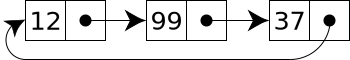
\includegraphics[width=.5\textwidth]{Circularly-linked-list} }
      \mode<article>{ 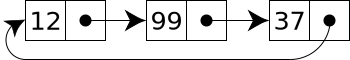
\includegraphics[width=.2\textwidth]{Circularly-linked-list} }
    \end{center}
  \end{block}
  \begin{block}{Doubly linked list}
    \begin{center}
      \mode<beamer>{ \includegraphics[width=.7\textwidth]{Doubly-linked-list} }
      \mode<article>{ \includegraphics[width=.3\textwidth]{Doubly-linked-list} }
    \end{center}
  \end{block}
\end{frame}

Linked lists are ill-suited for use cases where \emph{random access} is an important
operation. Instead, you use linked lists when \emph{iterating over the whole list} is
important and the \emph{dynamic addition and removal} of elements is
required. \citetitle[Sec.~6.1.3, \emph{Moving Through a Linked List}]{love2010linux}

See also: \citetitle{web:array-linkedlist}.

\begin{frame}{Circular doubly linked-lists}
  \begin{center}
    \mode<beamer>{ \includegraphics[width=\textwidth]{doubly-linked-list} }
    \mode<article>{ \includegraphics[width=.5\textwidth]{doubly-linked-list} }
  \end{center}
\end{frame}

See also: 
\begin{itemize}
\item \citetitle[Sec.~3.2.2.3, \emph{Doubly Linked Lists}]{bovet2005understanding};
\item \citetitle[Sec.~2.1, \emph{Common Kernel Data Types}]{rodriguez2005linux};
\item \citetitle{web:linkedlist};
\item \citetitle{web:klist}.
\end{itemize}

\begin{frame}[fragile=singleslide]
  \begin{block}{Things to note}
    \begin{enumerate}
    \item List is \emph{inside the data item} you want to link together.
    \item You \textbf{can put} ``\verb|struct list_head|'' \textbf{anywhere} in your structure.
    \item You \textbf{can name} ``\verb|struct list_head|'' \textbf{variable anything} you wish.
    \item You \textbf{can have} multiple lists!
    \end{enumerate}
  \end{block}
\end{frame}

\begin{frame}[fragile=singleslide]{Linked Lists}
  A linked list is initialized by using the \texttt{LIST\_HEAD} and
  \texttt{INIT\_LIST\_HEAD} macros
  \begin{block}{\texttt{include/linux/list.h}}%{\texttt{LIST\_HEAD} and \texttt{INIT\_ LIST\_HEAD}}
    \begin{center}
      \mode<beamer>{ \includegraphics[width=\textwidth]{list} }
      \mode<article>{ \includegraphics[width=.5\textwidth]{list} }      
    \end{center}
  \end{block}
  \begin{itemize}
  \item[Q1:] Why both \texttt{LIST\_HEAD\_INIT} and \texttt{INIT\_LIST\_HEAD}?
  \item[Q2:] Why \texttt{do-while}?
  \end{itemize}
\end{frame}

\paragraph{LIST\_HEAD}

When first encountering this, most people are confused because they have been taught to
implement linked lists by adding a pointer in a structure which points to the next similar
structure in the linked list. The drawback of this approach, and the reason for which the
kernel implements linked lists differently, is that you need to write code to handle
(adding/removing/etc) elements specifically for that data structure. Here, we can add a
struct \texttt{list\_head} field to any other data structure and, as we'll see shortly, make
it a part of a linked list. Moreover, if you want your data structure to be part of
several data structures, adding a few of these fields will work out just
fine\footnote{\url{http://kernelnewbies.org/FAQ/LinkedLists}}. \citetitle{kernelnewbies:FAQ/L72}

\subparagraph{Why is there a need to declare \texttt{LIST\_HEAD\_INIT} and
  \texttt{INIT\_LIST\_HEAD} they both seem to do the same thing?}

\begin{itemize}
\item An example \citetitle[Sec.~6.1.1, \emph{Defining a linked list}]{love2010linux}.
\item \texttt{LIST\_HEAD\_INIT} initializes one of these list head structure thingamajigs at
  compile time and so it doesn't actually generate any code, but stores constant values in
  a structure of which the address is known and
  fixed\footnote{\url{http://ubuntuforums.org/archive/index.php/t-1591281.html}}. \citetitle{ubuntuforums:linkl47}

  On the other hand, \texttt{INIT\_LIST\_HEAD} takes a pointer and so it could be a
  structure that is dynamically allocated, e.g. with ``\texttt{malloc}'' or one that is passed into
  your function... and then it does it's stuff at run time.
\item \texttt{LIST\_HEAD\_INIT} is a static initializer, \texttt{INIT\_LIST\_HEAD} is a
  function (in 2.6.11 it's still a macro). They both initialise a \texttt{list\_head} to be
  empty \footnote{\url{http://stackoverflow.com/questions/10262017/linux-kernel-list-list-head-init-vs-init-list-head}}. \citetitle{stackoverflow:c-Lin84}

  If you are statically declaring a \texttt{list\_head}, you should use
  \texttt{LIST\_HEAD\_INIT}, e.g.:

  \begin{center}
\begin{ccode}
static struct list_head mylist = INIT_LIST_HEAD(mylist);
\end{ccode}
  \end{center}
  You should use \texttt{INIT\_LIST\_HEAD()} for a list head that is dynamically allocated,
  usually part of another structure. There are many examples in the kernel source.
\item \textbf{My understanding:} compile time list head initialization is better for
  kernel memory management e.g. slab allocation.
\item See also: \citetitle{wiki:malloc}
\end{itemize}

\begin{frame}{Example}
  \begin{center}
    \mode<beamer>{ \includegraphics[width=.5\textwidth]{fox-struct} }
    \mode<article>{ \includegraphics[width=.3\textwidth]{fox-struct} }
  \end{center}
  \begin{block}{The list needs to be initialized before in use}
    \begin{itemize}
    \item Run-time initialization
      \begin{center}
        \mode<beamer>{ \includegraphics[width=.8\textwidth]{fox-dynamic} }
        \mode<article>{ \includegraphics[width=.5\textwidth]{fox-dynamic} }
      \end{center}
    \item Compile-time initialization
      \begin{center}
        \mode<beamer>{ \includegraphics[width=.7\textwidth]{fox-static} }
        \mode<article>{ \includegraphics[width=.5\textwidth]{fox-static} }
      \end{center}
    \end{itemize}
  \end{block}
\end{frame}

See also:
\begin{itemize}
\item \citetitle[Sec.~6.1.4, \emph{The Linux Kernel's Implementation}]{love2010linux}
\item About \texttt{kmalloc()}, see \citetitle[Sec.~8.1, \emph{The Real Story of
    kmalloc}]{corbet05ldd}
\item \texttt{GFP MASK} \citetitle{web:pagealloc}
\end{itemize}

\begin{frame}
  \begin{block}{The \texttt{do while(0)} trick}
    \begin{center}
      \mode<beamer>{ \includegraphics[width=.7\textwidth]{macro} }
      \mode<article>{ \includegraphics[width=.5\textwidth]{macro} }
    \end{center}
  \end{block}
\end{frame}

\paragraph{do...while(0)}

\begin{center}
  \includegraphics[width=.6\textwidth]{do-while}
\end{center}

See also:
\begin{itemize}
\item \citetitle{web:dowhile}
\item \citetitle{web:dowhile2}
\item \citetitle{web:dowhile3}
\end{itemize}
  
\begin{frame}[fragile=singleslide]
  \begin{block}{After \texttt{INIT\_LIST\_HEAD} macro is called}
    \begin{center}
      \mode<beamer>{ \mbox{
          \includegraphics[width=.25\textwidth]{list-head-2}\qquad
          \includegraphics[width=.72\textwidth]{list} }}
      \mode<article>{ \mbox{
          \includegraphics[width=.2\textwidth]{list-head-2}\qquad
          \includegraphics[width=.5\textwidth]{list} }}    
    \end{center}
  \end{block}
  Example: to start an empty \texttt{fox} list  
  \begin{center}
\begin{ccode}
static LIST_HEAD(fox_list);
\end{ccode}
  \end{center}
\end{frame}

\begin{frame}[fragile=singleslide]
  \begin{block}{Manipulating linked lists}
    \begin{itemize}
    \item To add a new member into \texttt{fox\_list}:
      \begin{itemize}
      \item[] \mintinline{c}{list_add(&new->list,&fox_list);}
        \begin{itemize}
        \item \mintinline{c}{fox_list->next->prev = new->list;}
        \item \mintinline{c}{new->list->next = fox_list->next;}
        \item \mintinline{c}{new->list->prev = fox_list;}
        \item \mintinline{c}{fox_list->next = new->list;}
        \end{itemize}
      \item[] \mintinline{c}{list_add_tail(&f->list,&fox_list);}
      \end{itemize}
    \item To remove an \mintinline{c}{old} node from list:
      \begin{itemize}
      \item[] \mintinline{c}{list_del(&old->list);}
        \begin{itemize}
        \item \mintinline{c}{old->list->next->prev = old->list->prev;}
        \item \mintinline{c}{old->list->prev->next = old->list->next;}
        \end{itemize}
      \end{itemize}
    \item a lot more...
    \end{itemize}
  \end{block}
\end{frame}

This function adds the new node to the given list immediately after the head node.

\begin{center}
  \mintinline{c}|list_add(struct list_head *new, struct list_head *head)|
\end{center}

Because the list is circular and generally has no concept of \emph{first} or \emph{last}
nodes, you can pass any element for \texttt{head}. If you do pass the ``\texttt{last}'' element,
however, this function can be used to implement a stack \citetitle[Sec.~6.1.5,
\emph{Manipulating Linked Lists}]{love2010linux}.

\begin{frame}[fragile=singleslide]{List Traversing}
  \begin{center}
\begin{ccode}
struct list_head *p;
list_for_each(p,fox_list){ ... }
\end{ccode}
  \end{center}
  \begin{block}{\texttt{list\_for\_each}}
    \begin{center}
      \mode<beamer>{ \includegraphics[width=\textwidth]{list2} }
      \mode<article>{ \includegraphics[width=.8\textwidth]{list2} }
    \end{center}
  \end{block}
  Not so useful. Usually we want the pointer to the container struct.
\end{frame}

\begin{frame}[fragile=singleslide]
  \begin{center}
    \mode<beamer>{ \includegraphics[width=.5\textwidth]{fox-struct} }
    \mode<article>{ \includegraphics[width=.3\textwidth]{fox-struct} }
  \end{center}
  \begin{itemize}
  \item[Q:] Given a pointer to \emph{\texttt{list}}, how to get a pointer to \emph{\texttt{fox}}?
    \begin{center}
      \mintinline{c}|f = list_entry(p, struct fox, list);|
    \end{center}
  \end{itemize}
  \begin{block}{\texttt{list\_entry(ptr, type, member)}}
    \begin{center}
      \mode<beamer>{ \includegraphics[width=\textwidth]{list-entry} }
      \mode<article>{ \includegraphics[width=.7\textwidth]{list-entry} }
    \end{center}
  \end{block}
\end{frame}

The code above deserves some explanation (Also read \citetitle{web:containerof}).

\begin{itemize}
\item \mintinline{c}{container_of(ptr,type,member)}: We have the address of the
  \mintinline{c}{struct list_head} field inside of another data structure (let's say
  \mintinline{c}{struct task_struct} for sake of example). The first line of the macro
  casts the value \texttt{0} into a pointer of the encapsulating data structure type
  (\mintinline{c}{struct task_struct} in our example). We use this pointer to access the
  field in that data structure which corresponds to our \verb|list_head| and get
  its type with the macro \texttt{typeof} to declare a pointer \texttt{mptr} initialized
  to the value contained in \texttt{ptr}. \citetitle{web:linkedlist}
\item How Does This Work? See \citetitle{web:klist}
\item \mintinline{c}{list_entry(ptr,type,member)}: \citetitle{web:klist2}
\end{itemize}

\begin{frame}{\texttt{list\_for\_each\_entry(pos, head, member)}}
  \begin{center}
    \mode<beamer>{ \includegraphics[width=\textwidth]{fox-lfee} }
    \mode<article>{ \includegraphics[width=.8\textwidth]{fox-lfee} }
  \end{center}
  \begin{block}{\texttt{list\_for\_each\_entry(pos, head, member)}}
    \begin{center}
      \mode<beamer>{ \includegraphics[width=\textwidth]{list-for-each-entry} }
      \mode<article>{ \includegraphics[width=.8\textwidth]{list-for-each-entry} }
    \end{center}
  \end{block}
\end{frame}

% \begin{frame}{Examples}{--- kernel/workqueue.c}
%   \begin{block}{The kernel adds \code{wq->list} to the system-wide list of work queues}
%     \begin{itemize}
%     \item[] \cfbox{red}{\code{list\_add(\&wq->list, \&workqueues);}}
%     \end{itemize}
%   \end{block}
%   \begin{block}{adds \code{work->entry} to the end of the list \code{cwq->worklist}}
%     \begin{itemize}
%     \item[] \cfbox{red}{\code{list\_add\_tail(\&work->entry, \&cwq->worklist);}}
%     \end{itemize}
%   \end{block}
%   \begin{block}{deleting an element from a list}
%     \begin{itemize}
%     \item[] \cfbox{red}{\code{list\_del(\&wq->list);}}
%     \end{itemize}
%   \end{block}
% \end{frame}

% \begin{itemize}
% \item \citetitle[Sec.~2.1.1]{rodriguez2005linux}.
% \item \citetitle[See.~sec 4.8, \emph{Work Queues},]{bovet2005understanding}
% \end{itemize}

\subsubsection{Queues}

Ref: \citetitle[Sec 6.2, \emph{Queues}]{love2010linux}

\begin{frame}{Queue (FIFO)}
  \begin{minipage}{.73\linewidth}
    \begin{block}{Circular buffer}
      \begin{description}
      \item[Empty:] $in == out$
      \item[Full:] $(in+1) \% BUFFER\_SIZE == out$
      \end{description}
    \end{block}
    Can be lock-free.
  \end{minipage}\hfill
  \begin{minipage}{.25\linewidth}
    \begin{center}
      \mode<beamer>{ \includegraphics[width=\textwidth]{circular} }
      \mode<article>{ \includegraphics[width=\textwidth]{circular} }
    \end{center}
  \end{minipage}
\end{frame}

See also: \citetitle{wiki:circular-buf}

\begin{frame}{KFIFO}
  \begin{block}{\texttt{include/linux/kfifo.h}}
    \begin{center}
      \mode<beamer>{ \includegraphics[width=\textwidth]{kfifo-struct} }
      \mode<article>{ \includegraphics[width=.9\textwidth]{kfifo-struct} }
    \end{center}
  \end{block}
  The \emph{spinlock} is rarely needed.
\end{frame}

\begin{frame}
  Initialization:
  \mode<beamer>{
    \begin{itemize}
    \item[] \includegraphics[width=.7\textwidth]{kfifo-alloc}
    \item[] \includegraphics[width=.7\textwidth]{kfifo-init}
    \end{itemize} }
  \mode<article>{
    \begin{itemize}
    \item[] \includegraphics[width=.4\textwidth]{kfifo-alloc}
    \item[] \includegraphics[width=.4\textwidth]{kfifo-init}
    \end{itemize} }
  \begin{block}{Example: to have a \texttt{PAGE\_SIZE}-sized queue}
    \begin{center}
      \mode<beamer>{ \includegraphics[width=.8\textwidth]{kfifo-alloc2} }
      \mode<article>{ \includegraphics[width=.6\textwidth]{kfifo-alloc2} }
    \end{center}
  \end{block}
\end{frame}

See also: \citetitle[Sec.~6.2.2, \emph{Creating a queue}, p97]{love2010linux}

\begin{frame}{\texttt{kfifo} operations}
  \begin{center}
    \mode<beamer>{ \includegraphics[width=.95\textwidth]{kfifo-op} }
    \mode<article>{ \includegraphics[width=.7\textwidth]{kfifo-op} }
  \end{center}
\end{frame}

\begin{frame}{Example}
  \begin{enumerate}
  \item To enqueue 32 integers into \emph{\texttt{fifo}}
    \begin{center}
      \mode<beamer>{ \includegraphics[width=.6\textwidth]{kfifo-in} }
      \mode<article>{ \includegraphics[width=.4\textwidth]{kfifo-in} }
    \end{center}
  \item To dequeue and print all the items in the queue
    \begin{center}
      \mode<beamer>{ \includegraphics[width=.8\textwidth]{kfifo-out} }
      \mode<article>{ \includegraphics[width=.5\textwidth]{kfifo-out} }
    \end{center}
  \end{enumerate}
\end{frame}

\begin{itemize}
\item \mintinline{c}{kfifo_in()}: This function copies the \emph{\texttt{len}} bytes
  starting at \emph{\texttt{from}} into the queue represented by
  \emph{\texttt{fifo}}. \citetitle[Sec.~6.2.3 \emph{Enqueuing Data}, p98]{love2010linux}
  \begin{itemize}
  \item On success it returns the number of bytes enqueued.
  \item If less than \emph{\texttt{len}} bytes are free in the queue, the function copies
    only up to the amount of available bytes.Thus the return value can be less than
    \emph{\texttt{len}} or even zero, if nothing was copied.
  \end{itemize}
\item \mintinline{c}{kfifo_out()}: This function copies at most \emph{\texttt{len}} bytes
  from the queue pointed at by \emph{\texttt{fifo}} to the buffer pointed at by
  \emph{\texttt{to}}. \citetitle[Sec.~6.2.4, \emph{Dequeuing Data}, p98]{love2010linux}
  \begin{itemize}
  \item On success the function returns the number of bytes copied.
  \item If less than \emph{\texttt{len}} bytes are in the queue, the function copies less
    than requested.
  \end{itemize}
\end{itemize}

% \subsubsection{Maps}
% \label{sec:maps}

% \citetitle[Sec 6.3, \emph{Maps}]{love2010linux}

% \begin{frame}{Maps}
%   \begin{itemize}
%   \item Associative array
%   \item Implementation
%     \begin{itemize}
%     \item Hash tables
%     \item Binary search trees
%     \end{itemize}
%   \item Operations
%     \begin{itemize}
%     \item \code{add(key, value)}
%     \item \code{remove(key)}
%     \item \code{value = lookup(key)}
%     \end{itemize}
%   \end{itemize}
% \end{frame}

\subsubsection{Binary Trees}

Ref: \citetitle[Sec.~6.4, \emph{Binary Trees}]{love2010linux}

\begin{frame}{Trees}
  \begin{itemize}
  \item Used in Linux memory management
    \begin{itemize}
    \item fast store/retrieve a single piece of data among many
    \end{itemize}
  \item generally implemented as \emph{linked lists} or \emph{arrays}
  \item the process of moving through a tree --- \emph{traversing}
  \end{itemize}
\end{frame}

\begin{frame}{Binary Search Tree}
  \begin{center}
    \includegraphics[width=.2\textwidth]{Binary_search_tree}
  \end{center}
  \begin{block}{Properties:}
    \begin{itemize}
    \item The left subtree of a node contains only nodes with keys less than the node's
      key.
    \item The right subtree of a node contains only nodes with keys greater than the
      node's key.
    \item Both the left and right subtrees must also be binary search trees.
    \end{itemize}
  \end{block}
  Efficient in:
  \begin{enumerate}
  \item searching for a given node
  \item in-order traversal (e.g. Left-Root-Right)
  \end{enumerate}
\end{frame}

See also:
\begin{itemize}
\item \citetitle{wiki:bin-search-tree}
\item \url{http://www.cs.duke.edu/~reif/courses/alglectures/skiena.lectures/lecture8.pdf}
\item \url{http://www.cse.iitk.ac.in/users/sbaswana/Courses/ESO211/bst.pdf/}
\item \url{http://www.personal.kent.edu/~rmuhamma/Algorithms/MyAlgorithms/binarySearchTree.htm}
\end{itemize}

\begin{frame}<beamer>
    \begin{tabu}{cc}
      Unbalanced binary tree&Balanced binary tree\\
      \includegraphics[width=.3\textwidth]{Unbalanced_binary_tree}&
      \includegraphics[width=.4\textwidth]{AVLtreef}\\
      &\\
      \multicolumn2{c}{Red-black tree}\\
      \multicolumn2{c}{\includegraphics[width=.6\textwidth]{Red-black-tree}}\\
      \tabuphantomline
    \end{tabu}
\end{frame}

\begin{figure}[!ht]
  \centering
  \begin{minipage}[b]{.2\linewidth}
    \includegraphics[width=\textwidth]{Unbalanced_binary_tree}
    \caption{Unbalanced binary tree}
  \end{minipage}\quad
  \begin{minipage}[b]{.3\linewidth}
    \includegraphics[width=\textwidth]{AVLtreef}
    \caption{Balanced binary tree}
  \end{minipage}\quad
  \begin{minipage}[b]{.3\linewidth}
    \includegraphics[width=\textwidth]{Red-black-tree}
    \caption{Red-black tree}
  \end{minipage}
\end{figure}

\begin{itemize}
\item A \emph{balanced binary search tree} is a binary search tree in which the depth of
  all leaves differs by at most one.
\item A \emph{self-balancing binary search tree} is a binary search tree that attempts, as
  part of its normal operations,to remain (semi) balanced.
\end{itemize}

See also:
\begin{itemize}
\item \citetitle{wiki:tree}
\item \citetitle{wiki:bin-tree}
\item \citetitle{wiki:bin-search-tree}
\item \citetitle{wiki:avl-tree}
\item \citetitle{wiki:rbtree}
\item \citetitle{wiki:big-o}
\end{itemize}

\begin{frame}
  \mode<beamer>{
    \begin{center}
      \includegraphics[width=.2\textwidth]{Red-black-tree}
    \end{center} }
  \begin{description}
  \item[Red-black tree] A type of \emph{self-balancing BST} in which each node has a red
    or black color attribute.
  \end{description}  
  \begin{block}{Properties to make it \emph{semi-balanced}:}
    \begin{enumerate}
    \item All nodes are either red or black
    \item Leaf nodes are black (root's color)
    \item Leaf nodes do not contain data (NULL)
    \item All non-leaf nodes have two children
    \item If a node is red, both its children are black
    \item When traversing from the root node to a leaf, each path contains the same number
      of black nodes
      % \item $O(log(n))$
    \end{enumerate}
    These properties ensure that \emph{the deepest leaf has a depth of no more than double that
    of the shallowest leaf}.
  \end{block}
\end{frame}

\begin{itemize}
\item Property 5 implies that on any path from the root to a leaf, red nodes must not be
  adjacent.  However, any number of black nodes may appear in a sequence.
\item Taken together, these properties ensure that the deepest leaf has a depth of no more
  than double that of the shallowest leaf. Consequently, the tree is always
  semi-balanced. Why this is true is surprisingly simple. First, by property five, a red
  node cannot be the child or parent of another red node. By property six, all paths
  through the tree to its leaves have the same number of black nodes.The longest path
  through the tree alternates red and black nodes.Thus the shortest path, which must have
  the same number of black nodes, contains only black nodes.Therefore, the longest path
  from the root to a leaf is no more than double the shortest path from the root to any
  other leaf. \citetitle[p105]{love2010linux}
\item \href{http://www.cs.auckland.ac.nz/\char`~jmor159/PLDS210/red\_black.html}{\emph{Data
      structure and algorithms, Sec 8.2, Red-black
      tree}}\footnote{\url{http://www.cs.auckland.ac.nz/~jmor159/PLDS210/red_black.html}}
\item \href{http://www.ece.uc.edu/\char`~franco/C321/html/RedBlack/redblack.html}{Red-black tree
    Java applet demo}
  \footnote{\url{http://www.ece.uc.edu/~franco/C321/html/RedBlack/redblack.html}}
\end{itemize}

\begin{frame}
  \begin{block}{Advantages}
    \begin{itemize}
    \item faster real-time bounded worst case performance for insertion and deletion
      \begin{itemize}
      \item usually at most two rotations% and three rotations, respectively, to balance the tree
      \end{itemize}
    \item slightly slower (but still $O(log n)$) lookup time
    \end{itemize}
  \end{block}
  \begin{block}{Many red-black trees in use in the kernel}
    \begin{itemize}
    \item The deadline and CFQ I/O schedulers employ rbtrees to track requests;
    \item the packet CD/DVD driver does the same
    \item The high-resolution timer code uses an rbtree to organize outstanding timer
      requests
    \item The ext3 filesystem tracks directory entries in a red-black tree
    \item Virtual memory areas (VMAs) are tracked with red-black trees
    \item epoll file descriptors, cryptographic keys, and network packets in the
      ``hierarchical token bucket'' scheduler
    \end{itemize}
  \end{block}
\end{frame}

See also:
\begin{itemize}
\item \citetitle{web:rbtree}
\item \citetitle{web:rbtree2}
\end{itemize}

\begin{frame}[fragile=singleslide]
  \begin{block}{\texttt{<linux/rbtree.h>}}
    \begin{center}
      \mode<beamer>{ \includegraphics[width=.75\textwidth]{rbtree} }
      \mode<article>{ \includegraphics[width=.4\textwidth]{rbtree} }
    \end{center}
  \end{block}
  To create a new empty tree:
  \begin{center}
    \mintinline{c}{struct rb_root root = RB_ROOT;}
  \end{center}
\end{frame}

\begin{itemize}
\item \href{http://www.kerneltravel.net/jiaoliu/kern-rbtree.html}{Linux内核中的红黑树}\footnote{\url{http://www.kerneltravel.net/jiaoliu/kern-rbtree.html}}
\item ``\mintinline{c}{(struct rb_root){ NULL, }}'' is a compound literal
  \citetitle[Sec.~6.26]{web:gcc}. ``\mintinline{c}{{ NULL, }}'' is an \emph{initializer
    list} \citetitle[Sec.~6.7.8, p125, \emph{Initialization}]{ISO:C99}. It initializes the
  1\textsuperscript{st} element (a pointer) to \emph{\texttt{NULL}}, and initializes the rest
  (omitted) as if they are static objects: arithmetic types are initialized to \emph{\texttt{0}};
  pointers are initialized to \emph{\texttt{NULL}} \citetitle{web:ibm-c}.

  See also:
  \begin{itemize}
  \item \citetitle[Sec.~6.5.2.5, p75, \emph{Compound literals}]{ISO:C99}
  \item \citetitle[Sec.~6.27, \emph{Designated Initializers}]{ISO:C99}
  \end{itemize}
\end{itemize}

\begin{frame}{Example}
  \begin{center}
    \mode<beamer>{ \includegraphics[width=.4\textwidth]{fox-rbtree} }
    \mode<article>{ \includegraphics[width=.3\textwidth]{fox-rbtree} }
  \end{center}
  \begin{block}{Search}
    \begin{center}
      \mode<beamer>{ \includegraphics[width=\textwidth]{fox-search} }
      \mode<article>{ \includegraphics[width=.7\textwidth]{fox-search} }
    \end{center}
  \end{block}
\end{frame}

\begin{frame}{Example}
  \begin{block}{Searching for a specific page in the page cache}
    \begin{center}
      \mode<beamer>{ \includegraphics[width=\textwidth]{rb-search} }
      \mode<article>{ \includegraphics[width=.7\textwidth]{rb-search} }
    \end{center}
  \end{block}
\end{frame}

See also:
\begin{itemize}
\item \texttt{include/linux/rbtree.h}  
\item \citetitle[p106-107]{love2010linux}
\item \citetitle[Sec.~9.3, \emph{Memory Regions}]{bovet2005understanding}
\end{itemize}

\subsection{Assembly}

\begin{frame}{x86 Assembly}
  \begin{block}{The Pentium class x86 architecture}
    \begin{itemize}
    \item Data ordering is in Little Endian
    \item Memory access is in byte (8 bit), word (16 bit), double word (32 bit), and quad
      word (64 bit).
    \item the usual registers for code and data instructions can be broken down into three
      categories: \emph{control}, \emph{arithmetic}, and \emph{data}.
    \end{itemize}
  \end{block}
\end{frame}

\begin{frame}
  \begin{block}{Byte ordering is architecture dependent}
    Storing an int (\texttt{0x01234567}) at address \texttt{0x100}:
    \begin{center}
      \mode<beamer>{ \includegraphics[width=.7\textwidth]{endian} }
      \mode<article>{ \includegraphics[width=.5\textwidth]{endian} }
    \end{center}
  \end{block}
\end{frame}

See also: \citetitle{wiki:endianness}

\begin{frame}
  \begin{center}
    \mode<beamer>{ \includegraphics[width=.7\textwidth]{registers}}
    \mode<article>{ \includegraphics[width=.5\textwidth]{registers}}
  \end{center}
  \begin{block}{Three kinds of registers}
    \begin{enumerate}
    \item general purpose registers
    \item segment registers
    \item status/control registers
    \end{enumerate}
  \end{block}
\end{frame}

\begin{frame}
  \begin{block}{General purpose registers}
    \begin{multicols}{2}
      \begin{description}
      \item[EAX] \uline{A}ccumulator register
      \item[EBX] \uline{B}ase register
      \item[ECX] \uline{C}ounter for loop operations
      \item[EDX] \uline{D}ata register
        \columnbreak
      \item[ESI] \uline{S}ource \uline{I}ndex
      \item[EDI] \uline{D}estination \uline{I}ndex
      \item[ESP] \uline{S}tack \uline{P}ointer
      \item[EBP] \uline{B}ase \uline{P}ointer pointing to the top of previous stack frame
      \end{description}
    \end{multicols}
  \end{block}
\end{frame}

The eight general-purpose registers in the x86 processor family each have an unique
purpose. Each register has special instructions and opcodes which make fulfilling this
purpose more convenient or efficient. \citetitle{web:TheAr30}

\begin{description}
\item[EAX] There are three major processor architectures: register, stack, and
  accumulator. In a register architecture, operations such as addition or subtraction can
  occur between any two arbitrary registers. In a stack architecture, operations occur
  between the top of the stack and other items on the stack. In an accumulator
  architecture, the processor has single calculation register called the accumulator. All
  calculations occur in the accumulator, and the other registers act as simple data
  storage locations.

  The x86 processor does not have an accumulator architecture. It does, however, have an
  accumulator-like register: \texttt{EAX/AL}. Although most calculations can occur between
  any two registers, the instruction set gives the accumulator special preference as a
  calculation register.

  Since most calculations occur in the accumulator, the x86 architecture contains many
  optimized instructions for moving data in and out of this register. ... In your code,
  try to perform as much work in the accumulator as possible. As you will see, the
  remaining seven general-purpose registers exist primarily to support the calculation
  occurring in the accumulator.
\item[EBX] The base register gets its name from the \texttt{XLAT}
  instruction. \texttt{XLAT} looks up a value in a table using \texttt{AL} as the index
  and \texttt{EBX} as the base. \texttt{XLAT} is equivalent to
  \mintinline{nasm}{MOV AL, [BX+AL]},
  which is sometimes useful if you need to replace one 8-bit value with another from a
  table (Think of color look-up).

  So, of all the general-purpose registers, \texttt{EBX} is the only register without an
  important dedicated purpose. It is a good place to store an extra pointer or calculation
  step, but not much more.
\item[EDX] Of the seven remaining general-purpose registers, the data register,
  \texttt{EDX}, is most closely tied to the accumulator. Instructions that deal with over
  sized data items, such as multiplication, division, \texttt{CWD}, and \texttt{CDQ}, store the most
  significant bits in the data register and the least significant bits in the
  accumulator. In a sense, the data register is the 64-bit extension of the
  accumulator. The data register also plays a part in I/O instructions. In this case, the
  accumulator holds the data to read or write from the port, and the data register holds
  the port address.
\item[ECX] The count register, \texttt{ECX}, is the x86 equivalent of the ubiquitous
  variable \texttt{i}. Every counting-related instruction in the x86 uses \texttt{ECX}. The most
  obvious counting instructions are \texttt{LOOP}, \texttt{LOOPZ}, and \texttt{LOOPNZ}. Another
  counter-based instruction is \texttt{JCXZ}, which, as the name implies, jumps when the
  counter is 0. The count register also appears in some bit-shift operations, where it
  holds the number of shifts to perform. Finally, the count register controls the string
  instructions through the \texttt{REP}, \texttt{REPE}, and \texttt{REPNE} prefixes. In this
  case, the count register determines the maximum number of times the operation will
  repeat.

  Particularly in demos, most calculations occur in a loop. In these situations,
  \texttt{ECX} is the logical choice for the loop counter, since no other register has so
  many branching operations built around it. The only problem is that this register counts
  downward instead of up as in high level languages. Designing a downward-counting is not
  hard, however, so this is only a minor difficulty.
\item[EDI] Every loop that generates data must store the result in memory, and doing so
  requires a moving pointer. The destination index, EDI, is that pointer. The destination
  index holds the implied write address of all string operations. The most useful string
  instruction, remarkably enough, is the seldom-used \texttt{STOS}. \texttt{STOS} copies
  data from the accumulator into memory and increments the destination index. This
  one-byte instruction is perfect, since the final result of any calculation should be in
  the accumulator anyhow, and storing results in a moving memory address is a common task.

  See also: \citetitle{stack:stos}
\item[ESI] The source index, \texttt{ESI}, has the same properties as the destination
  index. The only difference is that the source index is for reading instead of
  writing. Although all data-processing routines write, not all read, so the source index
  is not as universally useful. When the time comes to use it, however, the source index
  is just as powerful as the destination index, and has the same type of instructions.

  In situations where your code does not read any sort of data, of course, using the
  source index for convenient storage space is acceptable.
\item[ESP \& EBP] When a block of code calls a function, it pushes the
  parameters and the return address on the stack. Once inside, function sets the base
  pointer equal to the stack pointer and then places its own internal variables on the
  stack. From that point on, the function refers to its parameters and variables relative
  to the base pointer rather than the stack pointer. Why not the stack pointer?  For some
  reason, the stack pointer lousy addressing modes. In 16-bit mode, it cannot be a
  square-bracket memory offset at all. In 32-bit mode, it can be appear in square brackets
  only by adding an expensive SIB byte to the opcode.

  In your code, there is never a reason to use the stack pointer for anything other than
  the stack. The base pointer, however, is up for grabs. If your routines pass parameters
  by register instead of by stack (they should), there is no reason to copy the stack
  pointer into the base pointer. The base pointer becomes a free register for whatever you
  need.
\end{description}

\begin{frame}
  \begin{block}{Segment registers}
    \begin{description}
    \item[CS] Code segment
    \item[SS] Stack segment
    \item[DS,ES,FS,GS] Data segment
    \end{description}
  \end{block}
  \begin{block}{A memory address is an offset in a segment}
    \begin{description}
    \item[ES:EDI] references memory in the ES (extra segment) with an offset of the value in the EDI
    \item[DS:ESI]
    \item[CS:EIP]
    \item[SS:ESP] 
    \end{description}
  \end{block}
\end{frame}

\begin{frame}
  \begin{block}{State/Control registers}
    \begin{description}
    \item[EFLAGS] Status, control, and system flags
    \item[EIP] The instruction pointer, contains an offset from CS (CS:EIP)
    \end{description}
  \end{block}
  \begin{block}{FLAGS}
    \begin{tabular}{|l|l|l|l|l|l|l|l|l|l|l|l|l|l|l|l|}
      \hline
      15&&&&11&&&&7&6&&&&&&0\\\hline
      -&-&-&-&O&D&I&T&S&Z&-&A&-&P&-&C\\\hline
    \end{tabular}
    \begin{multicols}{2}
      \begin{description}
      \item[CF] Carry flag
      \item[ZF] Zero flag
      \item[SF] Sign flag, Negative flag
      \item[OF] Overflow flag
      \end{description}
    \end{multicols}
  \end{block}
\end{frame}

See also: \citetitle{wiki:eflags}

\begin{frame}
  \begin{block}{Control Instructions \scriptsize{(Intel syntax)}}
    \begin{small}{\ttfamily
      \begin{tabular}{lll}
        \textbf{Instruction}&\textbf{Function}&\textbf{EFLAGS}\\\hline
        je&Jump if equal&$ZF=1$\\
        jg&Jump if greater&$ZF=0$\\
        &&$SF=OF$\\
        jge&Jump if greater or equal&$SF=OF$\\
        jl&Jump if less&$SF\ne{}OF$\\
        jle&Jump if less or equal&$ZF=1$\\
        jmp&Unconditional jump&unconditional
      \end{tabular}}
    \end{small}
  \end{block}
  \begin{block}{Example \scriptsize{(Intel syntax)}}
    \begin{center}
      \mode<beamer>{ \includegraphics[width=\textwidth]{asm2} }
      \mode<article>{ \includegraphics[width=.5\textwidth]{asm2} }
    \end{center}
  \end{block}
\end{frame}

\begin{frame}[fragile=singleslide]
  Data can be moved
  \begin{itemize}
  \item between registers
  \item between registers and memory
  \item from a constant to a register or memory, but
  \item \textbf{NOT} from one memory location to another
  \end{itemize}
  \begin{block}{Data instructions \scriptsize{(Intel syntax)}}
    \begin{enumerate}
    \item \mintinline{nasm}{mov eax, ebx}
      \begin{itemize}
      \item[] Move 32 bits of data from \texttt{ebx} to \texttt{eax}
      \end{itemize}
    \item \mintinline{nasm}{mov eax, WORD PTR[data3]}
      \begin{itemize}
      \item[] Move 32 bits of data from memory variable \texttt{data3} to \texttt{eax}
      \end{itemize}
    \item \mintinline{nasm}{mov BYTE PTR[char1], al}
      \begin{itemize}
      \item[] Move 8 bits of data from \texttt{al} to memory variable \texttt{char1}
      \end{itemize}
    \item \mintinline{nasm}{mov eax, 0xbeef}
      \begin{itemize}
      \item[] Move the constant value \texttt{0xbeef} to \texttt{eax}
      \end{itemize}
    \item \mintinline{nasm}{mov WORD PTR[my_data], 0xbeef}
      \begin{itemize}
      \item[] Move the constant value \texttt{0xbeef} to the memory variable
          \texttt{my\_data}
      \end{itemize}
    \end{enumerate}
  \end{block}
\end{frame}

\begin{frame}[fragile=singleslide]
  \begin{block}{Address operand syntax \scriptsize{(AT\&T syntax)}}
    \begin{center}
      \mintinline{gas}{ADDRESS_OR_OFFSET(%BASE_OR_OFFSET, %INDEX, MULTIPLIER)}
    \end{center}
    \begin{itemize}
    \item up to 4 parameters
      \begin{itemize}
      \item \texttt{ADDRESS\_OR\_OFFSET} and \texttt{MULTIPLIER} must be
          \textbf{constants}
      \item \texttt{\%BASE\_OR\_OFFSET} and \texttt{\%INDEX} must be
          \textbf{registers}
      \end{itemize}
    \item all of the fields are optional
      \begin{itemize}
      \item if any of the pieces is left out, substituted it with zero
      \end{itemize}
    \item final address =
      \begin{itemize}
      \item[] \scriptsize{\texttt{ADDRESS\_OR\_OFFSET + \%BASE\_OR\_OFFSET + \%INDEX * MULTIPLIER}}
      \end{itemize}
    \end{itemize}
  \end{block}
\end{frame}

\begin{frame}[fragile=singleslide]
  \begin{block}{Why so complicate?}
    To serve several \emph{addressing modes}
    \begin{description}
    \item[direct addressing mode] \mintinline{gas}{movl ADDRESS, %eax}
      \begin{itemize}
      \item load data at \texttt{ADDRESS} into \texttt{\%eax}
      \end{itemize}
    \item[indexed addressing mode] \mintinline{gas}{movl START(,%ecx,1), %eax}
        \begin{itemize}
        \item[-] \texttt{START} -- starting address;\qquad - \texttt{\%ecx} -- offset/index
        \end{itemize}
    \item[indirect addressing mode] \mintinline{gas}{movl (%eax), %ebx}
      \begin{itemize}
      \item load data at address pointed by \texttt{\%eax} into \texttt{\%ebx}
      \item \texttt{\%eax} contents an address pointer
      \end{itemize}
    \item[base pointer addressing mode] \mintinline{gas}{movl 4(%eax), %ebx}
    \end{description}
  \end{block}
  \begin{description}
  \item[immediate mode] \mintinline{gas}|movl $12, %eax|%$
    \begin{itemize}
    \item[without \texttt{\$}] Direct addressing
    \end{itemize}
  \end{description}
\end{frame}

\begin{frame}[fragile=singleslide]
  \begin{minipage}{.65\linewidth}
    \begin{block}{indexed addressing mode}
      \begin{center}
        \mintinline{gas}{movl START(,%ecx,1), %eax}
      \end{center}
      \begin{description}
      \item[\texttt{START}] starting address
      \item[\texttt{\%ecx}] offset/index
      \end{description}
    \end{block}
    \begin{block}{\mintinline{gas}{START(,INDEX,MULTIPLIER)}:}
      \begin{itemize}
      \item to access the 4\textsuperscript{th} byte from location \texttt{2002}
        \begin{itemize}
        \item[] $2002(,3,1) = 2002+3\times{}1 = 2005$
        \end{itemize}
      \item to access the 4\textsuperscript{th} word from location \texttt{2002}
        \begin{itemize}
        \item[] $2002(,3,4)= 2002+3\times{}4 = 2014$
        \end{itemize}
      \end{itemize}
    \end{block}
  \end{minipage}\hfill
  \begin{minipage}{.29\linewidth}
    \begin{center}
      \mode<beamer>{ \includegraphics[width=\textwidth]{indexed-addressing} }
      \mode<article>{ \includegraphics[width=.5\textwidth]{indexed-addressing} }
    \end{center}
  \end{minipage}
\end{frame}

In \emph{indexed addressing mode}, if you have a set of numbers starting at location
\texttt{2002}, you can cycle between each of them using an index register.

The \emph{multiplier} allows you to access memory a byte at a time or a word at a time (4
bytes).

\begin{itemize}
\item[e.g.] If you are accessing an entire word, your index will need to be multiplied by
  4 to get the exact location of the fourth element from your address.

  For example, if you wanted to access the fourth byte from location \texttt{2002}, you
  would load your index register with \texttt{3} (remember, we start counting at
  \texttt{0}) and set the multiplier to \texttt{1} since you are going a byte at a
  time. This would get you location \texttt{2005}. However, if you wanted to access the
  fourth word from location \texttt{2002}, you would load your index register with
  \texttt{3} and set the multiplier to \texttt{4}. This would load from location
  \texttt{2014} - the fourth word. Take the time to calculate these yourself to make sure
  you understand how it works.
\end{itemize}

See also: \citetitle[Sec.~2.5, \emph{Data Accessing Methods}]{bartlett2009programming}

\begin{frame}
  \begin{block}{Example \scriptsize{(AT\&T syntax)}}
    \begin{center}
      \mode<article>{ \includegraphics[width=.5\textwidth]{asm3} }
      \mode<beamer>{ \includegraphics[width=.6\textwidth]{asm3} }
    \end{center}
  \end{block}
  \begin{itemize}
  \item each word is 4 bytes long
  \item stack grows downward
  \item \texttt{mov\uline{l}} --- long, 32 bits
  \item \texttt{\%\uline{e}ax} --- extended, 32 bits
  \end{itemize}
\end{frame}

\begin{itemize}
\item \texttt{4(\%esp)} --- base pointer addressing mode.
  \begin{center}
    \texttt{4(\%esp) = 4(\%esp, , ) = 4 + \%esp + 0*0}
  \end{center}
\end{itemize}

\begin{frame}
  \begin{block}{Example \scriptsize{(AT\&T syntax)}}
    \mode<beamer>{ \includegraphics[width=\textwidth]{asm} }
    \mode<article>{ \includegraphics[width=.5\textwidth]{asm} }
    % \cfbox{red}{\code{movl -4(\%ebp, \%edx, 4), \%eax}}
    %     \begin{itemize}
    %     \item {\scriptsize{load \code{*(ebp - 4 + (edx * 4))} into \code{eax}}}
    %     \end{itemize}
  \end{block}
\end{frame}

\begin{itemize}
\item \emph{GAS Syntax} \citetitle{wikibooks-gas}.
\item \citetitle[Sec.~3.5, \emph{Addressing Modes}]{bartlett2009programming}
\item \texttt{movl} --- Data operation. load data into somewhere(register/memory).
\item \texttt{leal} --- Address operation. load effective address. \citetitle[Appendix.~B,
  p259]{bartlett2009programming}.
\end{itemize}

\begin{frame}
  \begin{block}{Example --- stack setup \scriptsize{(AT\&T syntax)}}
      \begin{center}
        \mode<article>{ \includegraphics[width=.6\textwidth]{asm4} }
        \mode<beamer>{ \includegraphics[width=\textwidth]{asm4} }
      \end{center}
  \end{block}
\end{frame}

\subsubsection{Assembly Language Examples}

\begin{frame}{Stack Setup}
  \begin{block}{Before executing a function, the program}
    \begin{itemize}
    \item pushes all of the parameters for the function onto the stack. Then
    \item issues a \emph{call} instruction indicating which function it wishes
      to start. The call instruction does two things
      \begin{enumerate}
      \item pushes the address of the next instruction (return address) onto the
        stack.
      \item modifies the instruction pointer (\texttt{\%eip}) to point to the start
        of the function.
      \end{enumerate}
    \end{itemize}
  \end{block}
\end{frame}

See also: \citetitle[Sec.~4.3, \emph{Assembly-Language Functions using the C Calling
    Convention}, p54]{bartlett2009programming}.

\begin{frame}[fragile=singleslide]
  \begin{block}{At the time the function starts...}
    The stack looks like this:
    \begin{small}
\begin{verbatim}
          Parameter #N
          ...
          Parameter 2
          Parameter 1
          Return Address <- (%esp)
\end{verbatim}
    \end{small}
  \end{block}
\end{frame}

\begin{frame}[fragile=singleslide]
  \begin{block}{The function initializes the \texttt{\%ebp}}
    \begin{small}
\begin{verbatim}
        pushl %ebp
        movl %esp, %ebp
\end{verbatim}
    \end{small}
    Now the stack looks like this:
    \begin{small}
\begin{verbatim}
        Parameter #N <- N*4+4(%ebp)
        ...
        Parameter 2 <- 12(%ebp)
        Parameter 1 <- 8(%ebp)
        Return Address <- 4(%ebp)
        Old %ebp <- (%esp) and (%ebp)
\end{verbatim}
    \end{small}
\end{block}
  each parameter can be accessed using base pointer addressing mode using the \texttt{\%ebp}
  register
\end{frame}

\begin{frame}[fragile=singleslide]%{Stack Setup}
  \begin{block}{The function reserves space for locals}
    \begin{center}
      \mintinline{gas}{subl $8, %esp}%$
    \end{center}
    Our stack now looks like this:
    \begin{small}
\begin{verbatim}
        Parameter #N <- N*4+4(%ebp)
        ...
        Parameter 2 <- 12(%ebp)
        Parameter 1 <- 8(%ebp)
        Return Address <- 4(%ebp)
        Old %ebp <- (%ebp)
        Local Variable 1 <- -4(%ebp)
        Local Variable 2 <- -8(%ebp) and (%esp)
\end{verbatim}
    \end{small}
\end{block}
\end{frame}

\begin{frame}[fragile=singleslide]
  \begin{block}{When a function is done executing, it does three things:}
    \begin{enumerate}
    \item stores its return value in \texttt{\%eax}
    \item resets the stack to what it was when it was called
    \item \texttt{ret} --- \mintinline{gas}{popl %eip}
        \#set \texttt{eip} to \emph{return address}
        % returns control back to wherever it was called from % This is done
        % using the ret instruction, which pops whatever value is at the top of the stack,
        % and
        % sets the instruction pointer, %eip, to that value.
    \end{enumerate}
  \end{block}
  \begin{center}
\begin{gascode}
        movl %ebp, %esp
        popl %ebp
        ret
\end{gascode}
  \end{center}
\end{frame}

\begin{frame}[fragile=singleslide]
  \begin{block}{After \texttt{ret}}
    \begin{small}
\begin{verbatim}
        Parameter #N
        ...
        Parameter 2
        Parameter 1 <- (%esp)
\end{verbatim}
  \end{small}
\end{block}
  \begin{block}{How about the \texttt{parameters}?}
    \begin{itemize}
    \item Under many calling conventions the items popped off the stack by the epilogue
      include the original argument values, in which case there usually are no further
      stack manipulations that need to be done by the caller.
    \item With some calling conventions, however, it is the caller's responsibility to
      remove the arguments from the stack after the return.
    \end{itemize}
  \end{block}
\end{frame}

The calling code also needs to pop off all of the parameters it pushed onto the stack in
order to get the stack pointer back where it was (you can also simply add \texttt{4 × number
  of paramters} to \texttt{\%esp} using the \texttt{addl} instruction, if you don't need the
values of the parameters anymore). \citetitle[p58]{bartlett2009programming}

See also: \citetitle[Sec.~4.3, \emph{Return processing}]{wiki:callstack}

\begin{frame}{Generating Assembly From C Code}
  \begin{minipage}{.22\linewidth}
    \begin{block}{\texttt{simple.c}}
      \begin{center}
        \mode<beamer>{ \includegraphics[width=.8\textwidth]{simpleC} }
        \mode<article>{ \includegraphics[width=.5\textwidth]{simpleC} }
      \end{center}
    \end{block}
    \begin{small}
      \begin{itemize}
      \item[\$] \texttt{gcc -S simple.c}
      \end{itemize}
    \end{small}
  \end{minipage}\qquad
  \begin{minipage}{.7\linewidth}
    \begin{block}{\texttt{simple.s} \scriptsize{(AT\&T syntax)}}
      \begin{center}
        \mode<article>{ \includegraphics[width=.7\textwidth]{simpleS} }
        \mode<beamer>{ \includegraphics[width=\textwidth]{simpleS} }
      \end{center}
    \end{block}
  \end{minipage}
\end{frame}

See also:
\begin{itemize}
\item[\$] \mintinline{sh}{info gas 'Pseudo Ops'}
\item \href{http://stackoverflow.com/questions/3564752/what-is-cfi-and-lfe-in-assembly-code-produced-by-gcc-from-c-program}{\emph{What
      is \texttt{.cfi} and \texttt{.LFE} in assembly code produced by GCC from c++ program?}}
  \footnote{\url{http://stackoverflow.com/questions/3564752/what-is-cfi-and-lfe-in-assembly-code-produced-by-gcc-from-c-program}}
  \begin{itemize}
  \item \texttt{.LFB} --- Local Function Begin
  \item \texttt{.LFE} --- Local Function End
  \end{itemize}
\item \href{http://stackoverflow.com/questions/7534420/gas-explanation-of-cfi-def-cfa-offset}{\emph{GAS: Explanation of \texttt{.cfi\_def\_cfa\_offset}}}
  \footnote{\url{http://stackoverflow.com/questions/7534420/gas-explanation-of-cfi-def-cfa-offset}}
\item \href{http://stackoverflow.com/questions/8478491/understanding-base-pointer-and-stack-pointers-in-context-with-gcc-output}{\emph{Understanding gcc generated assembly}}
  \footnote{\url{http://stackoverflow.com/questions/8478491/understanding-base-pointer-and-stack-pointers-in-context-with-gcc-output}}
\item \href{http://sourceware.org/binutils/docs/as/Pseudo-Ops.html\#Pseudo-Ops}{\emph{Assembler
    directives}}\footnote{\url{http://sourceware.org/binutils/docs/as/Pseudo-Ops.html\#Pseudo-Ops}}
\item \href{http://blog.mozilla.com/respindola/2011/05/12/cfi-directives/}{\emph{cfi directives}}
  \footnote{\url{http://blog.mozilla.com/respindola/2011/05/12/cfi-directives/}}
\end{itemize}

\begin{frame}{Outline of an Assembly Language Program}
  \begin{block}{Assembler directives (Pseudo-Ops)}
    Anything starting with a `\texttt{.}'
    \begin{description}
    \item[\texttt{.section .data}] starts the data section
    \item[\texttt{.section .text}] starts the text section
    \item[\texttt{.globl SYMBOL}] \ 
      \begin{itemize}
      \item[\texttt{SYMBOL}] is a \emph{symbol} marking the location of a program
      \item[\texttt{.globl}] makes the symbol visible to `\texttt{ld}'
      \end{itemize}
    \item[\texttt{LABEL:}] a \emph{label} defines a \emph{symbol}'s value (address)
    \end{description}
  \end{block}
\end{frame}

\begin{frame}{Generating Assembly From C Code}
  \begin{minipage}{.35\linewidth}
    \begin{block}{\texttt{simple.s} \scriptsize{(Oversimplified)}}
      \begin{center}
        \mode<beamer>{ \includegraphics[width=.9\textwidth]{simple2S} }
        \mode<article>{ \includegraphics[width=.5\textwidth]{simple2S} }
      \end{center}
    \end{block}
    \begin{block}{Operation Prefixes}
      \begin{itemize}
      \item[\$] constant numbers
      \item[\%] register
      \end{itemize}
    \end{block}
  \end{minipage}\qquad
  \begin{minipage}{.55\linewidth}
    \begin{block}{suffixes}
      \begin{description}
      \item[b] byte (8 bit)
      \item[s] short (16 bit integer) or single (32-bit floating point)
      \item[w] word (16 bit)
      \item[l] long (32 bit integer or 64-bit floating point)
      \item[q] quad (64 bit)
      \item[t] ten bytes (80-bit floating point)
      \end{description}
    \end{block}
  \end{minipage}
\end{frame}

\begin{center}
\begin{gascode}
pushl %ebp
 movl %esp, %ebp
 subl $8, %esp 
\end{gascode}
\end{center}

\begin{itemize}
\item These lines save the value of EBP on the stack, then
\item move the value of ESP into EBP, then
\item subtract 8 from ESP.
\item Note that \texttt{pushl} automatically decremented ESP by the appropriate length.
\item This sequence of instructions is typical at the start of a subroutine to save space
  on the stack for local variables; EBP is used as the base register to reference the
  local variables, and a value is subtracted from ESP to reserve space on the stack (since
  the Intel stack grows from higher memory locations to lower ones). In this case, eight
  bytes have been reserved on the stack.
\item See also: \citetitle[\emph{Call Stack}]{wiki:callstack}
\end{itemize}

\begin{frame}{Generating Assembly From C Code}
  \begin{minipage}{.32\linewidth}
      \begin{block}{\texttt{count.c}}
        \begin{center}
          \mode<beamer>{ \includegraphics[width=.9\textwidth]{count} }
          \mode<article>{ \includegraphics[width=.6\textwidth]{count} }
        \end{center}
      \end{block}
      \begin{itemize}
      \item[\$] \texttt{gcc -S count.c}
      \end{itemize}
  \end{minipage}\qquad
  \begin{minipage}{.59\linewidth}
      \begin{block}{\texttt{count.s} \scriptsize{(AT\&T syntax)}}
        \begin{center}
          \mode<article>{ \includegraphics[width=.8\textwidth]{count2} }
          \mode<beamer>{ \includegraphics[width=\textwidth]{count2} }
        \end{center}
      \end{block}    
  \end{minipage}
\end{frame}

\paragraph{Why \texttt{subl \$16, \%esp}?}

The answer is \emph{stack alignment}. The compiler by default keeps the stack boundary
aligned to 16 bytes. We can see this from the gcc man page :
\begin{verbatim}
-mpreferred-stack-boundary=num
     Attempt to keep the stack boundary aligned to a 2 raised
     to num byte boundary. If -mpreferred-stack-boundary is not specified,
     the default is 4 (16 bytes or 128 bits).
\end{verbatim}

\begin{frame}[fragile=singleslide]{Generating Assembly From C Code}
  \begin{minipage}{.5\linewidth}
      \begin{block}{\texttt{count.s} {\scriptsize (oversimplified)}}
        \begin{center}
          \mode<beamer>{ \includegraphics[width=\textwidth]{count2S} }
          \mode<article>{ \includegraphics[width=.5\textwidth]{count2S} }
        \end{center}
      \end{block}    
  \end{minipage}\quad
  \begin{minipage}{.4\linewidth}
\begin{gascode}
leave:
    movl %ebp, %esp
    popl %ebp

enter:
    pushl %ebp
    movl  %esp, %ebp
\end{gascode}
  \end{minipage}
\end{frame}

      % \begin{itemize}
      % \item \emph{assembler directives} --- The lines beginning with periods, like
      %   "\code{.file}", "\code{.def}", or "\code{.ascii}"
      %   \begin{itemize}
      %   \item commands that tell the assembler how to assemble the file.
      %   \item \code{.text} --- declares the start of a section of code
      %   \item \code{.globl main} --- tells the assembler that the label \emph{main} is a
      %   global label, which allows other parts of the program to see it.
      %   \end{itemize}
      % \item \emph{labels} --- The lines beginning with some text followed by a colon, like
      %   "\code{\_main:}"
      % \end{itemize}    

See also:
\begin{itemize}
\item \href{http://sock-raw.org/netsec/stack}{\emph{Stack
      Explained}}\footnote{\url{http://sock-raw.org/netsec/stack}}
\item \href{http://stackoverflow.com/questions/672461/what-is-stack-alignment}{\emph{what
      is “stack alignment”?}}
  \footnote{\url{http://stackoverflow.com/questions/672461/what-is-stack-alignment}}
\item
  \href{http://stackoverflow.com/questions/4175281/what-does-it-mean-to-align-the-stack}{\emph{What
      does it mean to align the stack?}}
  \footnote{\url{http://stackoverflow.com/questions/4175281/what-does-it-mean-to-align-the-stack}}
\item \citetitle[\emph{Data Structure Alignment}]{wiki:alignment}
\end{itemize}

\subsubsection{Inline Assembly}

\begin{frame}[fragile=singleslide]{Inline Assembly}
  \begin{block}{Construct}
    \begin{center}
\begin{ccode}
asm (assembler instructions
    : output operands     /* optional */
    : input operands      /* optional */
    : clobbered registers /* optional */
    );
\end{ccode}
    \end{center}
  \end{block}
  \begin{block}{Example}
    \begin{center}
\begin{ccode}
asm ("movl %eax, %ebx");
asm ("movl %eax, %ebx" :::);
\end{ccode}
    \end{center}
    
    Use \verb|__asm__| if the keyword \texttt{asm} conflicts with something in
    our program:
    \begin{center}
\begin{ccode}
__asm__ ("movl %eax, %ebx");
__asm__ ("movl %eax, %ebx" :::);
\end{ccode}
    \end{center}
  \end{block}
\end{frame}

\paragraph{Why inline?}

... reduces the function-call overhead. Functions are great from the point of view of
program management - they make it easy to break up your program into independent,
understandable, and reuseable parts.  However, function calls do involve the overhead of
pushing arguments onto the stack and doing the jumps (remember locality of reference -
your code may be swapped out on disk instead of in memory).  For high level languages,
it's often impossible for compilers to do optimizations across function-call boundaries.
However, some languages support inline functions or function macros.  These functions
look, smell, taste, and act like real functions, except the compiler has the option to
simply plug the code in exactly where it was called. This makes the program faster, but it
also increases the size of the code. There are also many functions, like recursive
functions, which cannot be inlined because they call themselves either directly or
indirectly. \citetitle[p227, \emph{Inline Functions}]{bartlett2009programming}

\paragraph{GCC Extended Assembly}

In basic inline assembly, we had only instructions. In extended assembly, we can also
specify the operands. It allows us to specify the input registers, output registers and a
list of clobbered registers. \emph{It is not mandatory to specify the registers to use, we
  can leave that headache to GCC and that probably fit into GCC's optimization scheme
  better}.

If there are a total of \texttt{n} operands (both input and output inclusive), then the
first output operand is numbered \texttt{0}, continuing in increasing order, and the last
input operand is numbered \texttt{n-1}. \citetitle{howto:gcc-inline-asm}

\begin{description}
\item[\texttt{\%0}] the 1\textsuperscript{st} output operand
\item[\texttt{\%(n-1)}] the last input operand
\end{description}


\begin{frame}
  \begin{block}{Example: \texttt{exit(0)}}
    \begin{center}
      \mode<beamer>{ \includegraphics[width=\textwidth]{exit-asm} }
      \mode<article>{ \includegraphics[width=.7\textwidth]{exit-asm} }
    \end{center}
  \end{block}
\end{frame}

\paragraph{Quick System Call Review}

To recap --- Operating System features are accessed through system calls. These are
invoked by setting up the registers in a special way and issuing the instruction
\texttt{int \$0x80}.  Linux knows which system call we want to access by what we stored in
the \texttt{\%eax} register. Each system call has other requirements as to what needs to
be stored in the other registers. System call number \texttt{1} is the \texttt{exit()}
system call, which requires the status code to be placed in
\texttt{\%ebx}. \citetitle[p28]{bartlett2009programming}

\begin{frame}
  \begin{block}{Example}
    \begin{center}
      \mode<beamer>{ \includegraphics[width=\textwidth]{asm-inline} }
      \mode<article>{ \includegraphics[width=.7\textwidth]{asm-inline} }
    \end{center}
  \end{block}
  \begin{itemize}
  \item \texttt{ee,ce,reg} are local variables that will be passed as parameters to the
    inline assembler
  \item ``\texttt{\_\_volatile\_\_}'' tells the compiler not to optimize the inline
    assembly routine
  \item ``\texttt{r}'' means \emph{register}; It's a constraint.
  \item ``\texttt{=}'' denotes an output operand, and it's \emph{write-only}
  \item Clobbered registers tell GCC that the value of \texttt{\%eax} and \texttt{\%ebx}
    are to be modified inside "asm", so GCC won't use these registers to store any other
    value.
  \end{itemize}
\end{frame}

\paragraph{Extended asm}

If in our code we touch (ie, change the contents) some registers and return from asm
without fixing those changes, something bad is going to happen. This is because GCC have
no idea about the changes in the register contents and this leads us to trouble,
especially when compiler makes some optimization. It will suppose that some register
contains the value of some variable that we might have changed without informing GCC, and
it continues like nothing happened. What we can do is either use those instructions having
no side effects or fix things when we quit or wait for something to crash. This is where
we want some extended functionality. Extended asm provides us with that
functionality. \citetitle[Sec.~4, \emph{Basic Inline}]{howto:gcc-inline-asm}

\subsection{Quirky C Language Usage}

\begin{frame}[fragile=singleslide]{Quirky C Language Usage}{\texttt{asmlinkage} and \texttt{fastcall}}
  \begin{block}{\texttt{asmlinkage}}
    \mintinline{c}{asmlinkage int sys_fork(struct pt_regs regs)}
    \begin{itemize}
    \item tells the compiler to pass parameters on the local stack.
    \end{itemize}
  \end{block}
  \begin{block}{\texttt{fastcall}}
    \mintinline{c}{fastcall unsigned int do_IRQ(struct pt_regs *regs)}
    \begin{itemize}
    \item tells the compiler to pass parameters in the general-purpose registers.
    \end{itemize}
  \end{block}
  Macro definition:
  \begin{itemize}
  \item \mintinline{c}{#define asmlinkage CPP_ASMLINKAGE __attribute__((regparm(0)))}
  \item \mintinline{c}{#define fastcall __attribute__((regparm(3)))}
  \end{itemize} 
\end{frame}

\paragraph{What is \texttt{asmlinkage}?}

This is a \texttt{\#define} for some gcc magic that tells the compiler that the function
should not expect to find any of its arguments in registers (a common optimization), but
only on the CPU's stack. Recall our earlier assertion that \texttt{system\_call} consumes
its first argument, the system call number, and allows up to four more arguments that are
passed along to the real system call. \texttt{system\_call} achieves this feat simply by
leaving its other arguments (which were passed to it in registers) on the stack. All
system calls are marked with the \texttt{asmlinkage} tag, so they all look to the stack for
arguments. Of course, in \texttt{sys\_ni\_syscall}'s case, this doesn't make any difference,
because \texttt{sys\_ni\_syscall} doesn't take any arguments, but it's an issue for most
other system calls. And, because you'll be seeing \texttt{asmlinkage} in front of many other
functions, I thought you should know what it was about. \citetitle{kernelnewbies:FAQ/a70}
  
It is also used to allow calling a function from assembly files.

\paragraph{Why \texttt{asmlinkage}?}
Quote from \href{http://forum.soft32.com/linux/asmlinkage-purposes-optimizations-ftopict516190.html}{\emph{\texttt{asmlinkage} purposes and optimizations}}\footnote{\url{http://forum.soft32.com/linux/asmlinkage-purposes-optimizations-ftopict516190.html}}

\begin{verbatim}
> Hi everybody, 
> I'm new to this group. I'm writing to make up a doubt that I have on 
> the "asmlinkage" symbol. 
> I know that this keyword must be written, for example, in the 
> prototype of a system call in order to say to the compiler that, when 
> we call this function, it must put all the parameters in the stack, 
> hence avoiding optimizations, e.g. passing parameters using registers. 
> 
> Now my question is: why we should avoid this kind of optimizations? 
> I mean, we pass parameters to a syscall by registers. Then, the 
> syscall dispatcher puts all of them into the stack and finally it 
> calls the real syscall code. So why we should prevent the real syscall 
> code to get its parameters from the registers? 

Code can internally use any calling convention it wants. It can use an
optimized calling convention. It can use a slow calling convention.
It doesn't matter, so long as all code uses the same calling convention.
When you call into code that's not being compiled along with your current
code, you have to somehow specify that you need to use the calling
convention that this code uses rather than the default calling convention
for the compiler you're using (which may or may not be the same).

When you have a boundary between different code units, such as between 
user-space code and system calls or between C code and assembly code, 
you must define some calling convention. To tell the compiler to use 
that calling convention, you must specify some keyword. 

The details of what that calling convention is or how it may or may 
not differ from the calling conventions the compiler uses for the rest 
of the code are irrelevant. System calls or assembly code require some 
fixed calling convention, so you have to specify it somehow. 
\end{verbatim}

See also:
\begin{itemize}
\item \citetitle{wiki:callingconvention}
\item
  \href{http://stackoverflow.com/questions/10060168/is-asmlinkage-required-for-a-c-function-to-be-called-from-assembly}{\emph{Is
      “asmlinkage”  required for a c function to be called from
    assembly?}}\footnote{\url{http://stackoverflow.com/questions/10060168/is-asmlinkage-required-for-a-c-function-to-be-called-from-assembly}}
\item \href{http://hi.baidu.com/fiction\_junru/blog/item/75ee131e94c397c3a78669d1.html}{\emph{\texttt{asmlinkage}}}\footnote{\url{http://hi.baidu.com/fiction_junru/blog/item/75ee131e94c397c3a78669d1.html}}
\end{itemize}

\begin{frame}[fragile=singleslide]{Quirky C Language Usage}{\texttt{UL}}
  \begin{itemize}
  \item[\texttt{UL}] tells the compiler to treat the value as a long value.
    \begin{itemize}
    \item This prevents certain architectures from overflowing the bounds of their datatypes.
    \item Using \texttt{UL} allows you to write architecturally independent code for large
      numbers or long bitmasks.
    \end{itemize}
  \end{itemize}
  \begin{block}{Example}
    \begin{itemize}
    \item[] \mintinline{c}{#define GOLDEN_RATIO_PRIME 0x9e370001UL}
    \item[] \mintinline{c}{#define ULONG_MAX (~0UL)}
    \item[] \mintinline{c}{#define SLAB_POISON 0x00000800UL /* Poison objects */}
    \end{itemize}
  \end{block}
\end{frame}

\texttt{\char`~0UL} means that complement of 0 is to be interpreted as an unsigned long
explicitly casted as an unsigned int.
$$\mathtt{\sim0UL = 0xffffffff = 4294967295}$$
Thats the largest value that can be in a 32 bit integer \citetitle{web:uin93}.

\begin{frame}[fragile=singleslide]{Quirky C Language Usage}{\texttt{static inline}}
  \begin{description}
  \item[\texttt{inline}] An \texttt{inline} function results in the compiler attempting to
    incorporate the function's code into all its callers.
  \item[\texttt{static}] Functions that are visible only to other functions in the same file
    are known as \emph{static functions}.
  \end{description}
  \begin{block}{Example}
    \mintinline{c}{static inline void prefetch(const void *x)}
  \end{block}
\end{frame}

See also:
\begin{itemize}
\item \href{http://www.greenend.org.uk/rjk/tech/inline.html}{\emph{Inline Functions in C}}\footnote{\url{http://www.greenend.org.uk/rjk/tech/inline.html}}
\item \citetitle{wiki:inlinefunction}
\end{itemize}

\begin{frame}{Quirky C Language Usage}{\texttt{const}}
  \begin{block}{\texttt{const} --- read-only}
    \texttt{const int *x}
    \begin{itemize}
    \item a pointer to a \texttt{const} integer
    \item the pointer can be changed but the integer cannot
    \end{itemize}
    \texttt{int const *x}
    \begin{itemize}
    \item a \texttt{const} pointer to an integer
    \item the integer can change but the pointer cannot
    \end{itemize}
  \end{block}
\end{frame}

\begin{frame}{Quirky C Language Usage}{\texttt{volatile}}
  \begin{minipage}{.44\linewidth}
    \begin{block}{Without \texttt{volatile}}
      \begin{center}
        \mode<article>{ \includegraphics[width=.7\textwidth]{volatile} }
        \mode<beamer>{ \includegraphics[width=\textwidth]{volatile} }
      \end{center}
    \end{block}
  \end{minipage}\hfill
  \begin{minipage}{.50\linewidth}
    However, \texttt{foo} might represent a location that can be changed by other elements
    of the computer system at any time, such as a hardware register of a device connected
    to the CPU.
  \end{minipage}
  \begin{itemize}
  \item[] To prevent the compiler from optimizing code, the \texttt{volatile} keyword is
    used:
    \begin{center}
      \texttt{static volatile int foo;}
    \end{center}
  \end{itemize}
\end{frame}

See also: \citetitle{wiki:volatile}

\subsection{Miscellaneous Quirks}

\begin{frame}[fragile=singleslide]{Miscellaneous Quirks}{\texttt{\_\_init}}
  \begin{small}
    \mintinline{c}{#define __init __attribute__ ((__section__ (".init.text")))}
  \end{small}
  \begin{itemize}
  \item The \verb|__init| macro tells the compiler that the associate function or variable
    is used only upon initialization.
  \item The compiler places all code marked with \verb|__init| into a special memory
    section that is freed after the initialization phase ends
  \end{itemize}
  \begin{block}{Example}
    \begin{small}
      \mintinline{c}{static int __init batch_entropy_init(int size, struct entropy_store *r)}
    \end{small}
  \end{block}
  Similarly,
  \begin{itemize}
    \item[] \verb|__initdata, __exit, __exitdata|
  \end{itemize}
\end{frame}

See also:
\begin{itemize}
\item \citetitle[Sec.~2.4, \emph{Hello World (part 3): The \_\_init and \_\_exit
    Macros}]{salzman07kernel}
\item \citetitle[Sec.~6.36, \emph{Variable Attributes}]{web:gcc}
\end{itemize}

%\begin{frame}{Miscellaneous Quirks}{ --- \code{likely(), unlikely()}}

\subsection{A Quick Tour of Kernel Exploration Tools}

\begin{frame}{Kernel Exploration Tools}
  \begin{description}
  \item[objdump] Display information about object files
    \begin{itemize}
    \item[\$] \texttt{objdump -S simple.o}
    \item[\$] \texttt{objdump -Dslx simple.o}
    \end{itemize}
  \item[readelf] Displays information about ELF files
    \begin{itemize}
    \item[\$] \texttt{readelf -h a.out}
    \end{itemize}
  \item[hexdump] ASCII, decimal, hexadecimal, octal dump
    \begin{itemize}
    \item[\$] \texttt{hd a.out}
    \end{itemize}
  \item[nm] List symbols from object files
    \begin{itemize}
    \item[\$] \texttt{nm a.out}
    \end{itemize}
  % \item \code{objcopy} Migrate object code from one platform, such as x86, to another, such as ARM
  \end{description}
\end{frame}

See also:
\begin{itemize}
\item \citetitle{wiki:elf}
\item \href{http://www.linuxforums.org/articles/understanding-elf-using-readelf-and-objdump\_125.html}{\emph{Understanding ELF using readelf and
    objdump}}\footnote{\url{http://www.linuxforums.org/articles/understanding-elf-using-readelf-and-objdump_125.html}}
\end{itemize}

\paragraph{How to decompress vmlinuz?}

To exam the kernel image with \texttt{objdump}, you have to decompress it first.
\begin{enumerate}
\item[\$] \verb|cp /boot/vmlinuz-3.7.0-rc3-next-20121029 /tmp/|
\item[\$] \verb^od -A d -t x1 vmlinuz-3.7.0-rc3-next-20121029 | grep '1f 8b 08 00'^

  The output should be something like this:
  \begin{center}
    \texttt{0016992}\qquad\texttt{f3 a5 fc 5e 8d 83 b4 91 4f 00 ff e0 1f 8b 08 00}
  \end{center}
\item[\$] \verb^dd if=vmlinuz bs=1 skip=17004 | zcat > vmlinux^
\item How did i calculated 17004 ?
  \begin{itemize}
  \item[] 0016992 + offset of GZ signature(\texttt{1f 8b 08 00}), i.e.
  \item[] 0016992 + 12
  \end{itemize}
\item[\$] \verb^dd if=vmlinuz-3.7.0-rc3-next-20121029 bs=1 skip=17004 | zcat > vmlinux^
\begin{verbatim}
5233764+0 records in
5233764+0 records out
5233764 bytes (5.2 MB) copied
\end{verbatim}
\item[\$] \verb|file vmlinux|
\item[\$] \verb|objdump -f vmlinux|
\end{enumerate}

See also: \url{http://comments.gmane.org/gmane.linux.kernel.kernelnewbies/42926}

\subsection{Kernel Speaks: Listen to Kernel Messages}

\begin{frame}\mode<beamer>{\frametitle{Listen To Kernel Messages}}
  \begin{description}
  \item[\texttt{printk()}] behaves almost identically to the C library \texttt{printf()} function
  \item[\texttt{dmesg}] print or control the kernel ring buffer
  \item[\texttt{/var/log/messages}] is where a majority of logged system messages reside
  \end{description}
\end{frame}

\lecture[boot]{boot}{boot}

\section{From Power Up To Bash Prompt}

\begin{frame}<beamer>
    \title{From Power Up To Bash Prompt}
    \author{Wang Xiaolin}
    \titlepage
    \vfill
    {\small\emoji{📧} \url{wx672ster+os@gmail.com} }
\end{frame}

\subsection{Motherboard Chipsets And The Memory Map}

Ref: \citetitle{duarte:gustavo2008chipsets}

\begin{frame}\mode<beamer>{\frametitle{Motherboard Chipsets And The Memory Map}}
  \begin{center}
    \mode<beamer>{ \includegraphics[width=\textwidth]{motherboardDiagram} }
    \mode<article>{ \includegraphics[width=.6\textwidth]{motherboardDiagram} }
  \end{center}
\end{frame}

\begin{frame}
  \begin{block}{Facts}
    \begin{itemize}
    \item The CPU doesn't know what it's connected to
      \begin{itemize}
      \item[-] CPU test bench?\quad{}network router?\quad{}toaster?\quad{}brain implant?
      \end{itemize}
    \item The CPU talks to the outside world through its pins
      \begin{itemize}
      \item[-] some pins to transmit the physical memory address
      \item[-] other pins to transmit the values
      \end{itemize}
    \item The CPU's gateway to the world is the front-side bus
    \end{itemize}
  \end{block}
  \begin{block}{Intel Core 2 QX6600}
    \begin{itemize}
    \item 33 pins to transmit the physical memory address
      \begin{itemize}
      \item[-] so there are $2^{33}$ choices of memory locations
      \end{itemize}
    \item 64 pins to send or receive data
      \begin{itemize}
      \item[-] so data path is 64-bit wide, or 8-byte chunks
      \end{itemize}
    \end{itemize}
    This allows the CPU to physically address 64GB of memory ($2^{33}\times{}8B$)
  \end{block}
\end{frame}

See also: \href{http://download.intel.com/design/processor/datashts/31559205.pdf}{\emph{Datasheet for Intel Core 2 Quad-Core Q6000
  Sequence}}\footnote{\url{http://download.intel.com/design/processor/datashts/31559205.pdf}}

\begin{frame}%{Motherboard Chipsets And The Memory Map}{ --- Facts}
  \begin{varwidth}{.59\textwidth}
    \textcolor{blue}{Some physical memory addresses are mapped away!}
    \begin{itemize}
    \item only the addresses, not the spaces
    \item Memory holes
      \begin{itemize}
      \item[-] $640KB \sim 1MB$
      \item[-] /proc/iomem
      \end{itemize}
    \item Memory-mapped I/O
      \begin{itemize}
      \item BIOS ROM
      \item video cards
      \item PCI cards
      \item ...
      \end{itemize}
    \end{itemize}
    This is why 32-bit OSes have problems using 4G of RAM.
  \end{varwidth}\hfill
  \begin{varwidth}{.39\textwidth}
    \begin{center}
      \includegraphics[width=1.2\textwidth]{boot-mem}
    \end{center}
  \end{varwidth}
  \vspace{1em}
  \begin{center}
    What if you don't have 4G RAM?
  \end{center}
\end{frame}

See also: \href{http://wiki.osdev.org/Memory_Map_(x86)}{\emph{Memory Map (x86)}}\footnote{\url{http://wiki.osdev.org/Memory_Map_(x86)}}

\begin{frame}%{Motherboard Chipsets And The Memory Map}{ --- Facts}
  \begin{block}{the northbridge}
    \begin{enumerate}
    \item receives a physical memory request
    \item decides where to route it
      \begin{itemize}
      \item[-] to RAM? to video card? to ...?
      \item[-] decision made via the \emph{memory address map}
        \begin{itemize}
        \item \texttt{/proc/iomem}
        \item it is built in \texttt{setup()}
        \end{itemize}
      \end{itemize}
    \end{enumerate}
  \end{block}
\end{frame}

% \begin{itemize}
% \item When is the memory address map built? \code{setup()}.
% \end{itemize}

\begin{frame}%{Motherboard Chipsets And The Memory Map}{ --- Facts}
  \begin{block}{The CPU modes}
    \begin{description}
    \item[real mode:] CPU can only address 1MB RAM
      \begin{itemize}
      \item 20-bit address, 1-byte data unit
      \end{itemize}
    \item[32-bit protected mode:] can address 4GB RAM
      \begin{itemize}
      \item 32-bit address, 1-byte data unit
      \end{itemize}
    \item[64-bit protected mode:] can address 64GB RAM (Intel Core 2 QX6600)
      \begin{itemize}
      \item 33 address pins, 8-byte data unit
      \end{itemize}
    \end{description}
  \end{block}
  \begin{itemize}
  \item[\$] \texttt{grep 'address sizes' /proc/cpuinfo}
  \end{itemize}
\end{frame}

The \emph{physical} stuff is determined by hard-core limits: the actual metal pins that
stick out of the processor. It is \emph{those} pins that limit the CPU to 64
gigabytes. That is completely independent of the operating system or even the mode
(real-mode, 32-bit protected, 64-bit) the CPU is running in. It's a physical limit. That
is the limit for which that little multiplication is done. There are 33 metal pins to
transmit an address and 8 metal pins to send and receive data. So
$2^{33}\times{} 2^3 = 2^{36} = 64 GB$.  The “unit” of transfer in this case is 8 bytes,
that's the smallest chunk of data the CPU can address on the physical bus. In actuality,
the CPU usually works in terms of cache lines, which hold 64 bytes in the Core 2s. Due to
performance, the CPU reads a whole cache line at a time. So if a program reads one byte,
the CPU actually reads 64 bytes and stores them in the cache.  The 4-gb limit is logical,
not physical. It happens because the registers and instructions in the CPU are limited to
32 bits \emph{when it's running in 32-bit mode}, which \emph{does} depend on the
OS. Programs need to be able to address individual bytes in memory, so the “unit” of
addressing is 1 byte. So \emph{that} equation becomes
$2^{32}\ addresses \times{} 1\ byte\ chunks = 2^{32}\ bytes$, or 4 GB total
addressing. (The comments in \citetitle{duarte:gustavo2008chipsets})

\subsection{How Computers Boot Up}

Ref: \citetitle{duarte:gustavo2008boot}

\begin{frame}{Bootstrapping}
  \begin{center}
    \mode<beamer>{ \includegraphics[width=\textwidth]{boot} }
    \mode<article>{ \includegraphics[width=.8\textwidth]{boot-bw} }
  \end{center}
  \begin{enumerate}
  \item bringing at least a portion of the OS into main memory, and
  \item having the processor execute it
  \item the initialization of kernel data structures
  \item the creation of some user processes, and
  \item the transfer of control to one of them
  \item[\$] \texttt{man 7 boot}
  \end{enumerate}
\end{frame}

\subsubsection{Motherboard power up}

\begin{frame}
  \begin{block}{Motherboard power up}
    \begin{enumerate}
    \item initializes motherboard firmwares (chipset, etc.)
    \item gets CPU running
    \end{enumerate}
  \end{block}
\end{frame}

\begin{frame}{Real mode}{CPU acts as a 1978 Intel 8086}
  \begin{varwidth}{.52\textwidth}
    \begin{itemize}
    \item any code can write to any place in memory
    \item only 1MB of memory can be addressed
    \item registers are initialized
      \begin{itemize}
      \item[-] \texttt{EIP} has \texttt{0xFFFFFFF0}, the \textcolor{blue}{reset vector}
      \item[-] at the reset vector, there is a \texttt{jump} instruction, jumping to the
        \emph{BIOS entry point} (\texttt{0xF0000}).%\ (960KB), 64KB below 1MB)
      \end{itemize}
    \end{itemize}
  \end{varwidth}\hfill
  \begin{varwidth}{.48\textwidth}
    \begin{center}
      \mode<beamer>{ \includegraphics[width=1.15\textwidth]{boot-mem} }
      \mode<article>{ \includegraphics[width=.7\textwidth]{boot-mem} }
    \end{center}
  \end{varwidth}
\end{frame}

See also:
\begin{itemize}
\item \citetitle{web:bios-rom}
\item \citetitle{web:boot-seq}
\item \citetitle{web:bios-rom2}
\item \citetitle{wiki:rst-vector}
\item \citetitle{web:boot-cpu}
\end{itemize}

\subsubsection{BIOS}

\begin{frame}\mode<beamer>{\frametitle{BIOS}}
  \begin{block}{BIOS uses Real Mode addresses}
    \begin{itemize}
    \item No GDT, LDT, or paging table is needed
      \begin{itemize}
      \item the code that initializes the GDT, LDT, and paging tables must run in Real Mode
      \end{itemize}
    \item Real mode address translation:
      $$\mathtt{segment number}\times{}2^4+\mathtt{offset}$$
      \begin{itemize}
      \item[e.g.] to translate \texttt{<FFFF:0001>} into physical address:
        $$FFFF \times{} 16 + 0001 = FFFF0 + 0001 = FFFF1$$
      \item[if:] \texttt{offset > 0xF} (overflow)
      \item[then:] $\mathtt{address \% 2^{20}}$ (wrap around)
      \item only 80286 and later x86 CPUs can address up to:
        $$FFFF0 + FFFF = 10FFEF$$
      \end{itemize}
    \end{itemize}
  \end{block}
\end{frame}

See also:
\begin{itemize}
\item \citetitle[Sec.~1.3, \emph{The BIOS}]{freebsd:archbook}
\item \citetitle{wiki:realmode}
\item \citetitle{osdev:realmode} 
\end{itemize}

\begin{frame}{CPU starts executing BIOS code}
  \begin{enumerate}
  \item POST
    \begin{itemize}
    \item an ACPI-compliant BIOS builds several tables that describe the hardware devices
      present in the system
    \end{itemize}
  \item initializes hardwares
    \begin{itemize}
    \item at the end of this phase, a table of installed PCI devices is displayed
    \end{itemize}
  \item find a boot device
  \item load MBR into \texttt{0x7c00}
  \item Jump to \texttt{0x7c00}
  \item MBR moves itself away from \texttt{0x7c00}% (fig~\ref{fig:boot-mem3})
  \end{enumerate}
  \begin{center}
    \mode<beamer>{
      \includegraphics[width=\textwidth]{mbr}
    } \mode<article>{
      \includegraphics[width=.6\textwidth]{mbr}
    }
  \end{center}
\end{frame}

\begin{varwidth}{.65\textwidth}
  \begin{itemize}
  \item The MBR includes a small boot loader, which is loaded into RAM starting from
    address \texttt{0x00007c00} by the BIOS.

    \begin{itemize}
    \item \href{http://www.glamenv-septzen.net/en/view/6}{Why \texttt{0x7c00}?}\footnote{\url{http://www.glamenv-septzen.net/en/view/6}}
    \end{itemize}

  \item This small program
    \begin{enumerate}
    \item moves itself to the address \texttt{0x00096a00},
      \begin{itemize}
      \item Why? because the boot loader may copy the boot sector of a boot
        partition into RAM (\texttt{0x7c00}) and execute it
      \end{itemize}
    \item sets up the real mode stack (ranging from \texttt{0x00098000} to
      \texttt{0x000969ff}),
    \item loads the second part of the boot loader into RAM starting from address
      \texttt{0x00096c00}, and jumps into it.
    \end{enumerate}
  \end{itemize}
\end{varwidth}\hfill
\begin{varwidth}{.3\textwidth}
  \includegraphics[width=\textwidth]{boot-mem3}
\end{varwidth}

\subsubsection{The Boot Loader}

\begin{frame}[fragile=singleslide]{GRUB}
  \begin{enumerate}
  \item GRUB stage 1 (in MBR) loads GRUB stage 2
  \item stage 2 reads GRUB configuration file, and presents boot menu
  \item loads the kernel image file into memory% (fig~\ref{fig:boot-mem3})
    \begin{itemize}
    \item can't be done in real mode, since it's bigger than 640KB
      \begin{itemize}
      \item BIOS supports \emph{unreal mode}
      \end{itemize}
    \item 1\textsuperscript{st} 512 bytes --- \texttt{INITSEG, 0x00090000}
    \item \texttt{setup()} --- \texttt{SETUPSEG, 0x00090200}
    \item load low --- \texttt{SYSSEG, 0x00010000}
    \item load high --- \texttt{0x00100000}
    \end{itemize}
  \item jumps to the kernel entry point (\mintinline{gas}{jmp trampoline})
    \begin{itemize}
    \item line 80 in \texttt{2.6.11/arch/i386/boot/setup.S}
    \end{itemize}
  \end{enumerate}
\end{frame}

``\mintinline{gas}{jmp trampoline}'' was used in 2.6.11 for calling \texttt{start\_of\_setup}. In
newer kernels, a \emph{2-byte jump} is used instead.

See also:
\begin{itemize}
\item \href{http://www.dedoimedo.com/computers/grub.html}{\emph{GRUB bootloader - Full
      tutorial}}\footnote{\url{http://www.dedoimedo.com/computers/grub.html}}
\item Kernel source v2.6.34:
  \href{http://lxr.linux.no/linux+v2.6.34/arch/x86/boot/header.S\#L112}{\emph{\texttt{header.S}}}\footnote{\url{http://lxr.linux.no/linux+v2.6.34/arch/x86/boot/header.S\#L112}}
\item \href{http://thestarman.pcministry.com/asm/2bytejumps.htm}{\emph{Using SHORT
      (Two-byte) Relative Jump
      Instructions}}\footnote{\url{http://thestarman.pcministry.com/asm/2bytejumps.htm}}
\item \href{http://www.groad.net/bbs/read.php?tid-3001.html}{\emph{2-byte jump in
      \texttt{header.S}}}\footnote{\url{http://www.groad.net/bbs/read.php?tid-3001.html}}
\end{itemize}

\paragraph{More about unreal mode}

Unreal Mode is a ``mode'' where the processor runs in real mode while the segment limit
does not equal 64KB (in most cases, its 4GB). Since real mode doesn't update the limit
field (of the cache), this state persists across segment register loads. Entering this
mode is achieved easily by entering protected mode (where the limit can be changed), load
the desired limit into the descriptor cache, then switch back to real
mode. \citetitle{osdev:descriptor-cache}

The benefits of unreal mode are quite well known: access to the 32-bit address space while
simultaneously being able to call BIOS and real mode programs. \citetitle{osdev:unrealmode2}

See also:
\begin{itemize}
\item \href{http://forum.osdev.org/viewtopic.php?f=1\&t=21179\&start=15}{A great post in OSDev forum: \emph{Unreal
  mode}}\footnote{\url{http://forum.osdev.org/viewtopic.php?f=1&t=21179&start=15}} that
deserves a detailed look.
\item OSDev:
  \href{http://files.osdev.org/mirrors/geezer/johnfine/segments.htm}{\emph{Segment
      Registers: Real mode vs. Protected mode}} covers \emph{unreal mode}, \emph{NULL
    selector}, \emph{mode
    switching}\footnote{\url{http://files.osdev.org/mirrors/geezer/johnfine/segments.htm}}.
\item \citetitle{osdev:realmode2}
\item \citetitle{wiki:unrealmode}
\item \citetitle{osdev:unrealmode}
\end{itemize}

\begin{figure}[h]
  \centering
  \includegraphics[width=.4\textwidth]{nonprogrammable}
  \caption{Descriptor cache register}
  \label{fig:cache-register}
\end{figure}

\paragraph{More about \emph{bootloader}:}
\begin{enumerate}
\item display a ``Loading'' message
\item load an initial portion of the kernel image from disk:
  \begin{enumerate}
  \item the first 512 bytes of the kernel image are put in RAM at address
    \texttt{0x00090000} (576K, \texttt{INITSEG})
    \begin{itemize}
    \item \mintinline{sh}{hd -n512 /boot/vmlinuz-3.2.0-1-amd64}
    \item \texttt{/usr/src/linux/arch/i386/boot/bootsect.S}
    \item it was a floppy boot loader, and no longer valid since 2.6
    \item nowadays to make a bootable floppy, you have to use a bootloader as you do with
      a hard disk
    \end{itemize}
  \item the code of the \texttt{setup()} function (see below) is put in RAM starting
    from address \texttt{0x00090200} ($576K+512$, \texttt{SETUPSEG})
  \end{enumerate}
\item load the rest of the kernel image from disk and puts the image in RAM starting from
  either low address \texttt{0x00010000} (64K, \texttt{SYSSEG}) (for small kernel images
  ($< 512K$) compiled with ``\mintinline{sh}{make zImage}'') or high address
  \texttt{0x00100000} (1M)(for big kernel images ($> 512K$) compiled with \mintinline{sh}{make
    bzImage}).
  \begin{description}
  \item[ISA hole:] Physical addresses ranging from \texttt{0x000a0000} (640K) to
    \texttt{0x000fffff} ($1M-1$) are usually reserved to BIOS routines and to map the
    internal memory of ISA graphics cards
  \end{description}
\item Jumps to the \texttt{setup()} code. (\texttt{/usr/src/linux/arch/i386/boot/setup.S})
\end{enumerate}

\begin{description}
\item[BIOS interrupt call] \mintinline{gas}{int $0x13} is oftenly seen in %$
  \texttt{2.6.11/arch/i386/boot/setup.S}.  \mintinline{gas}{INT 13H}, \mintinline{gas}{INT 13h}, or
  \mintinline{gas}{INT 19} is shorthand for BIOS interrupt call $\mathtt{13_{hex}}$, the
  20\textsuperscript{th} interrupt vector in an x86-based computer system. The BIOS
  typically sets up a real mode interrupt handler at this vector that provides
  sector-based hard disk and floppy disk read and write services using
  cylinder-head-sector (CHS) addressing.
\end{description}

See also: \citetitle[Sec.~3, \emph{How Boot Loaders Work}]{web:linuxbootloader}

\begin{frame}{Memory At Bootup Time}
  \begin{varwidth}{.7\textwidth}
    \begin{block}{The kernel image}
      \begin{itemize}
      \item \texttt{/boot/vmlinuz-x.x.x-x-x}
      \item has been loaded into memory by the boot loader using the BIOS disk I/O
        services
      \item The image is split into two pieces:
        \begin{itemize}
        \item a small part containing the real-mode kernel code is loaded below the 640K
          barrier
        \item the bulk of the kernel, which runs in protected mode, is loaded after the
          first megabyte of memory
        \end{itemize}
      \end{itemize}
    \end{block}
  \end{varwidth}\hfill
  \begin{varwidth}{.25\textwidth}\label{fig:boot-mem3}
    \begin{center}
      \mode<beamer>{ \includegraphics[width=1.3\textwidth]{boot-mem3} }
      \mode<article>{ \includegraphics[width=\textwidth]{boot-mem3} }
    \end{center}
  \end{varwidth}
\end{frame}

See also: \citetitle[\emph{boot-time memory arrangement}]{linux2.6.25protocol}.

\subsection{The Kernel Boot process}

\subsubsection{\texttt{setup()}}

\begin{frame}{The \texttt{setup()} Function}
  boots and loads the executable image to ($\mathtt{0x9000\ll 4}$) and jumps to
  ($\mathtt{0x9020\ll 4}$)
  \begin{center}
    \mode<beamer>{ \includegraphics[width=\textwidth]{setup2} }
    \mode<article>{ \includegraphics[width=.7\textwidth]{setup2} }
  \end{center}
  \begin{itemize}
  \item \texttt{2.6.11/arch/i386/boot/setup.S}
  \item Re-initialize all the hardware devices
  \item Sets the A20 pin (turn off \emph{wrapping around})
  \item Sets up a provisional IDT and a provisional GDT
  \item \texttt{PE=1, PG=0} in \texttt{cr0}
  \item jump to \texttt{startup\_32()}
  \end{itemize}
\end{frame}

See also:
\begin{itemize}
\item \citetitle{newbies:kernelstart}
\item \citetitle{blogspot:bootprocess}
\item \citetitle{blogspot:bootprocess2}
\end{itemize}

\begin{itemize}
\item \emph{Kernel attributes} are stored at the end of the boot block
  (1\textsuperscript{st} sector).
  (line \href{http://lxr.linux.no/linux+v2.6.11/arch/i386/boot/bootsect.S\#L90}{90} in
    \texttt{bootsect.S})
\end{itemize}  

\paragraph{The \texttt{setup()} function details:}

\begin{enumerate}
\item Builds system's physical memory map \citetitle[sec.~1.1, \emph{Memory
    Detection}]{abhishek2002memory}. See also:
  \begin{itemize}
  \item \texttt{2.4.19/arch/i386/boot/setup.S}, line
    \href{http://lxr.linux.no/linux-old+v2.4.19/arch/i386/boot/setup.S\#L289}{289-389}
  \item \texttt{2.6.11/arch/i386/boot/setup.S}, line
    \href{http://lxr.linux.no/linux+v2.6.11/arch/i386/boot/setup.S\#L302}{302-347}
  \item See also: \citetitle{wiki:e820}
  \item \url{http://www.uruk.org/orig-grub/mem64mb.html}
  \end{itemize}
\item Sets the keyboard repeat delay and rate
\item Initializes the video adapter card
\item Reinitializes the disk controller and determines the hard disk parameters
\item Checks for an IBM Micro Channel bus (MCA)
\item Checks for a PS/2 pointing device (bus mouse)
\item Checks for Advanced Power Management (APM ) BIOS support
\item If the BIOS supports the Enhanced Disk Drive Services (EDD ), builds a table in RAM
  describing the hard disks available in the system
\item If the kernel image was loaded low in RAM (at physical address \texttt{0x00010000}),
  the function moves it to physical address \texttt{0x00001000} (was used by boot loader).
  \begin{description}
  \item[Why?] This step is necessary because to be able to store the kernel image on a
    floppy disk and to reduce the booting time, the kernel image stored on disk is
    compressed, and the decompression routine needs some free space to use as a temporary
    buffer following the kernel image in RAM.  \citetitle[Sec.~A.3, \emph{Middle Ages: the
      \texttt{setup()} Function}]{bovet2005understanding}
    \begin{itemize}
    \item \texttt{BOOTSEG = 0x07C0}. This is 27K above \texttt{0x1000}. It was too small to
      hold the kernel image. After boot loader is done, \texttt{BOOTSEG (0x7C00)} is
      free. So kernel image can be stuffed here.
    \end{itemize}
  \item[Memory layout] \citetitle{blogspot:bootprocess}\,
    \begin{description}
    \item[uncompressed image:] ... Later, all the kernel is moved from \texttt{0x10000}
      (64K) to \texttt{0x1000} (4K). This move overwrites BIOS data stored in RAM, so BIOS
      calls can no longer be performed. We don't care because linux doesn't use BIOS to
      access the hardware. The first physical page is not touched because it is the
      so-called ``zero-page'', used in handling virtual memory.  At this point,
      \texttt{setup.S} enters protected mode and jumps to \texttt{0x1000}, where the kernel
      lives. All the available memory can be accessed now, and the system can begin to
      run.

      The steps just described were once the whole story of booting when the kernel was
      small enough to fit in half a megabyte of memory --- the address range between
      \texttt{0x10000} and \texttt{0x90000}. As features were added to the system, the kernel
      became larger than half a megabyte and could no longer be moved to
      \texttt{0x1000}. Thus, code at \texttt{0x1000} is no longer the Linux kernel, instead
      the “gunzip” part of the gzip program resides at that address.
      
    \item[Compressed image (zImage):] When the kernel is moved to \texttt{0x1000} (4K),
      \texttt{head.S} in the compressed directory is sitting at this address. It's in charge
      of gunzipping the kernel, this done by a function \texttt{decompress\_kernel()},
      defined in \texttt{compressed/misc.c}, which in turns calls \texttt{inflate()} which
      writes its output starting at address \texttt{0x100000} (1MB). High memory can now
      be accessed, because \texttt{setup.S} han take us to the protected mode now.  After
      decompression, \texttt{head.S} jumps to the actual beginning of the kernel. The
      relevant code is in \texttt{../kernel/head.S}. \texttt{head.S} (i.e., the code
      found at \texttt{0x100000}) can complete processor initialization and call
      \texttt{start\_ kernel()}.

      The boot steps shown above rely on the assumption that the compressed kernel can fit
      in half a megabyte of space. While this is true most of the time, a system stuffed
      with device drivers might not fit into this space. For example, kernels used in
      installation disks can easily outgrow the available space. To solve this problem
      problem bzImage kernel images were introduced.

    \item[Big Compressed Image (bzImage):] This kind of kernel image boots similarly to
      zImage, with a few changes.
    \end{description}
    When the system is loaded at \texttt{0x10000} (64K) a special helper routine is called
    which does some special BIOS calls to move the kernel to \texttt{0x100000}
    (1Mb). \texttt{setup.S} doesn't move the system back to \texttt{0x1000} (4K) but, after
    entering protected mode, jumps instead directly to address \texttt{0x100000} (1MB) where
    data has been moved by the BIOS in the previous step.  The decompresser found at 1MB
    writes the uncompressed kernel image into low memory until it is exhausted, and then
    into high memory after the compressed image.  The two pieces are then reassembled to
    the address \texttt{0x100000} (1MB). Several memory moves are needed to perform the task
    the address \texttt{0x100000} (1MB). Several memory moves are needed to perform the task
    correctly.
  \end{description}

  \begin{center}
    \includegraphics[width=.5\textwidth]{setup-func-1}
  \end{center}

  The default value of \texttt{code32} is \texttt{\_\_BOOT\_CS:0x1000} (\texttt{\_\_BOOT\_CS} =
  16). (Line
  \href{http://lxr.linux.no/linux+v2.6.11/arch/i386/boot/setup.S\#L855}{855-857})

  \begin{center}
    \includegraphics[width=.6\textwidth]{setup-func-2}
  \end{center}

  It will be changed to \texttt{\_\_BOOT\_CS:0x100000}.
  (Line \href{http://lxr.linux.no/linux+v2.6.11/arch/i386/boot/setup.S\#L594}{594-595})
    
  \begin{center}
    \includegraphics[width=.3\textwidth]{setup-func-3}
  \end{center}

  \texttt{\%cs:code32\_start} $\Rightarrow$ \texttt{\%cs:code32} = \texttt{0x10:0x100000} (for
  load high, i.e. \texttt{bzImage})
\item Sets the A20 pin \citetitle{wiki:a20} located on the 8042 keyboard controller (for
  switching to pmode)
\item Sets up a provisional Interrupt Descriptor Table (IDT) \citetitle{wiki:idt} and a
  provisional Global Descriptor Table (GDT) \citetitle{wiki:gdt}.
  \begin{itemize}
  \item line \href{http://lxr.linux.no/linux+v2.6.11/arch/i386/boot/setup.S\#L792}{792} in
      \texttt{setup.S}
  \item line \href{http://lxr.linux.no/linux+v2.6.11/include/asm-i386/segment.h\#L83}{83-89}
      in \texttt{include/asm-i386/segment.h}
  \end{itemize}
  The provisional GDT is created with 2 useful entries, each covering the whole 4GB
  address space \citetitle[Sec.~1.2, \emph{Provisional GDT}]{abhishek2002memory}. The code that
  loads the GDT is:    
  \begin{center}
    \includegraphics[width=.6\textwidth]{setup-func-4}
  \end{center}

  \begin{itemize}
  \item \texttt{\%ds = \%cs = SETUPSEG = 0x9020}
  \item \texttt{\$gdt} --- beginning address of the GDT table (somewhere offsetting in
    \texttt{\%ds}). Its actual value will be determined at assemble time by the assembler
    \citetitle[p24]{bartlett2009programming}
  \item \texttt{gdt\_48}: a label in \texttt{setup.S} (Line
    \href{http://lxr.linux.no/linux+v2.6.11/arch/i386/boot/setup.S\#L1006}{1006}). \texttt{gdt\_48+2}
    will be filled with the \emph{gdt base} computed above.
  \item \texttt{lgdt}: loads the value in \texttt{gdt\_48} into \texttt{GDTR}
  \item \texttt{gdt\_48 = limit,base} $\Rightarrow$ \texttt{GDTR}
    \begin{itemize}
    \item \texttt{limit = gdt\_end - gdt - 1 = 31} (16 bits)
    \item \texttt{base = \%ds $\ll$ 4 + gdt} (32 bits)
    \end{itemize}
  \end{itemize}

  \begin{center}
    \includegraphics[width=.5\textwidth]{setup-func-5}
  \end{center}

  \begin{itemize}
  \item \texttt{gdt}: the provisional GDT has 4 entries.
    \begin{itemize}
    \item The 1\textsuperscript{st} and 2\textsuperscript{nd} entries are initialized to
      0\footnote{\texttt{.fill REPEAT,SIZE,VALUE}}
      (Line \href{http://lxr.linux.no/linux+v2.6.11/arch/i386/boot/setup.S\#L983}{983}), as
      required by Intel.
      \begin{center}
        \mintinline{gas}{.fill GDT_ENTRY_BOOT_CS,8,0}
      \end{center}
    \item The 3\textsuperscript{rd} is \texttt{\_\_BOOT\_CS}
    \item The 4\textsuperscript{th} is \texttt{\_\_BOOT\_DS}
    \end{itemize}
    Calculate the linear base address of the kernel GDT (table) and load the GDT pointer
    register with its base address and limit. \citetitle[\emph{Prepare to move to protected
      mode}]{howto:init}
    \begin{figure}[h]
      \centering
      \includegraphics[width=.3\textwidth]{gdt-boot}
      \caption{Provisional GDT in RAM}
      \label{fig:gdt-boot}
    \end{figure}
    \begin{itemize}
    \item This early kernel GDT describes kernel code as 4 GB, with base address 0,
      code/readable/executable, with granularity of 4 KB.
      \begin{figure}[h]
        \centering
        \includegraphics[width=.6\textwidth]{gdt-entry-cs}
        \caption{Code segment descriptor value: \texttt{0x00CF9A000000FFFF}}
        \label{fig:cs}
      \end{figure}
    \item The kernel data segment is described as 4 GB, with base address 0,
      data/readable/writable, with granularity of 4 KB.
      \begin{figure}[h]
        \centering
        \includegraphics[width=.6\textwidth]{gdt-entry-ds}
        \caption{Data segment descriptor value: \texttt{0x00CF92000000FFFF}}
        \label{fig:ds}
      \end{figure}
    \end{itemize}
  \end{itemize}
\item Resets the floating-point unit (FPU), if any.
\item Reprograms the Programmable Interrupt Controllers (PIC) to mask all interrupts,
  except IRQ2 which is the cascading interrupt between the two PICs.
\item Switches the CPU from Real Mode to Protected Mode by setting the \texttt{PE} bit in
  the \texttt{cr0} status register. The \texttt{PG} bit in the \texttt{cr0} register is cleared,
  so paging is still disabled. (Line
  \href{http://lxr.linux.no/linux+v2.6.11/arch/i386/boot/setup.S\#L832}{832-833})

  \begin{center}
    \includegraphics[width=.4\textwidth]{setup-func-6}
  \end{center}

  \begin{itemize}
  \item \texttt{lmsw} --- Load Machine Status Word (part of
    \texttt{cr0}) \citetitle[Ch.~17]{intel86}
  \item in later kernel (e.g. 2.6.34) the switching code is like this
    (\href{http://lxr.linux.no/linux+v2.6.34/arch/x86/boot/pmjump.S\#L39}{line 39-41 in
      pmjump.S}):
      
    \begin{center}
      \includegraphics[width=.4\textwidth]{setup-func-7}
    \end{center}
      
    Line
    \href{http://lxr.linux.no/linux+v2.6.34/arch/x86/include/asm/processor-flags.h\#L29}{29}
    in \texttt{processor-flags.h}:
    \begin{center}
\begin{ccode}
#define X86_CR0_PE 0x00000001
\end{ccode}    
    \end{center}
  \end{itemize}
  \textbf{NOTE:} We are now in 32-bit protected mode. From now on, the address translation
  will be done by looking up the GDT table.
\item Jumps to the \texttt{startup\_32()} assembly language
  function. (Line \href{http://lxr.linux.no/linux+v2.6.11/arch/i386/boot/setup.S\#L854}{854})
  \begin{center}
    \includegraphics[width=.5\textwidth]{setup-func-8}
  \end{center}

  \begin{itemize}
  \item \mintinline{gas}{jmpi 0x100000, __BOOT_CS} (far jump)
    \begin{itemize}
    \item jump to \texttt{0x10:0x100000} (segment number: \texttt{0x10}; offset:
      \texttt{0x100000}.)
    \end{itemize}
  \item At the end of the initial assembly code in \texttt{arch/i386/boot/setup.S} a jump
    to offset \texttt{0x100000} in segment \texttt{KERNEL\_CS} is called. This is where
    the version of \mintinline{c}{startup_32()} found in
    \texttt{arch/i386/boot/compress-ed/head.S}. But the jump is a little tricky, as we
    haven't yet reloaded the \texttt{CS} register, the default size of the target offset
    still is 16 bit. However, using an operand prefix (\texttt{0x66}), the CPU will
    properly take our 48 bit far pointer [\mintinline{gas}{.byte 0x66, 0xea}]. \citetitle{blogspot:bootprocess}
  \end{itemize}
\end{enumerate}

% \begin{frame}{The real-mode kernel header}
%   The action starts in \emph{the real-mode kernel header}
%   \begin{itemize}
%   \item This region of memory is used to implement the Linux boot protocol between the
%     boot loader and the kernel
%   \item \emph{Documentation/i386/boot.txt}
%   \end{itemize}
% \end{frame}

% \begin{frame}{The real-mode kernel header}
%   \begin{block}{\emph{arch/i386/boot/bootsect.S}}
%     \begin{center}
%       \includegraphics[width=.7\textwidth]{kernel-header}
%     \end{center}
%   \end{block}
%   \cfbox{red}{hd -n512 /boot/vmlinuz-x.x.x-x-x}
% \end{frame}

\subsubsection{\texttt{startup\_32()}}

\begin{frame}{\texttt{setup() -> startup\_32()}}%{The real mode entry point}
  \begin{block}{\texttt{startup\_32()} for compressed kernel}
    \begin{itemize}
    \item in \texttt{arch/i386/boot/compressed/head.S}
      \begin{itemize}
      \item physically at
        \begin{itemize}
        \item[]\texttt{0x00100000} --- load high, or
        \item[]\texttt{0x00001000} --- load low
        \end{itemize}
      \item does some basic register initialization
      \item \texttt{decompress\_kernel()}
      \end{itemize}
    \item the uncompressed kernel image has overwritten the compressed one starting at 1MB
    \item jump to the protected-mode kernel entry point at 1MB of RAM ($\mathtt{0x10000\ll 4}$)
      \begin{itemize}
      \item \texttt{startup\_32()} for real kernel
      \end{itemize}
    \end{itemize}
  \end{block}
\end{frame}

\paragraph{Initializing registers}
(Line \href{http://lxr.linux.no/linux+v2.6.11/arch/i386/boot/compressed/head.S\#L31}{31}
in \texttt{head.S})

\begin{center}
  \includegraphics[width=.3\textwidth]{head-reg-init}
\end{center}

\begin{itemize}
\item \texttt{cld}: clear direction flag
\item \texttt{cli}: clear interrupt flag
\item \verb|lss stack_start, %esp|: load \texttt{\%ss} and \texttt{\%esp} pair
  (\texttt{\%ss:\%esp}) in a single instruction using the value stored in
  \texttt{stack\_start}.  (Line
  \href{http://lxr.linux.no/linux+v2.6.11/arch/i386/boot/compressed/head.S\#L40}{40} in
  \texttt{head.S})
  \begin{itemize}
  \item \texttt{lss} --- read a full pointer from memory and store it in the selected
    segment register:register pair. \citetitle[p332]{intel86}
  \end{itemize}
  % load values stored in \code{stack\_start} into \code{ss:esp}
\item \texttt{stack\_start} (Line
  \href{http://lxr.linux.no/linux+v2.6.11/arch/i386/boot/compressed/misc.c\#L296}{296-303}
  in \texttt{misc.c})

  \begin{center}
    \includegraphics[width=.6\textwidth]{stack-start}
  \end{center}

\item \texttt{STACK\_SIZE} = 4096
\item \texttt{\_\_BOOT\_DS} = 24 (segment selector) $\Rightarrow$ \texttt{\%ss}
  \begin{itemize}
  \item the 4\textsuperscript{th} (2\textsuperscript{nd} non-zero) entry in provisional
    GDT \citetitle[Sec.~1.2, \emph{Provisional GDT}]{abhishek2002memory}. Each entry is
    8 bytes.
  \end{itemize}
\item \texttt{\&user\_stack[4096]} $\Rightarrow$ \texttt{\%esp}
\end{itemize}

\paragraph{Clear BSS}

(Line
\href{http://lxr.linux.no/linux+v2.6.11/arch/i386/boot/compressed/head.S\#L55}{55} in
\texttt{head.S})

\begin{center}
  \includegraphics[width=.2\textwidth]{head-clr-bss}
\end{center}
  
\begin{itemize}
\item \href{http://www.cs.ubbcluj.ro/\char`~dadi/ac/doc/ng1d5fc.html}{\texttt{stosb}} copies the
  value in \texttt{AL} into the location pointed to by \texttt{ES:DI}. \texttt{DI} is then
  incremented (if the direction flag is cleared) or decremented (if the direction flag is
  set), in preparation for storing \texttt{AL} in the next location.
\item \texttt{rep} --- repeat
\item For \texttt{ecx} repetitions, stores the contents of \texttt{eax} into where \texttt{edi}
  points to, incrementing or decrementing \texttt{edi} (depending on the direction flag) by
  4 bytes each time. Normally, this is used for a memset-type operation.

  Usually, that instruction is simply written ``\mintinline{gas}{rep stosd}''. Experienced assembly
  coders know all the details mentioned above just by seeing that. \good{}%:-)

  ETA for completeness (thanks PhiS): Each iteration, \texttt{ecx} is decremented by 1, and
  the loop stops when it reaches zero. For \texttt{stos}, the only thing you will observe is
  that \texttt{ecx} is cleared at the end. \citetitle{stack:stos}
\end{itemize}

\begin{frame}{\texttt{startup\_32()} for real kernel}
  \begin{block}{\texttt{startup\_32()} in \texttt{arch/i386/kernel/head.S}}
    \begin{itemize}
    \item Zeroes the kernel BSS for protected mode
    \item sets up the final GDT
    \item builds provisional kernel page tables so that paging can be turned on
    \item enables paging (\texttt{cr3->PGDir; PG=1} in \texttt{cr0})
    \item initializes a stack
    \item \texttt{setup\_idt()} --- creates the final interrupt descriptor table
    \item \texttt{gdtr->GDT; idtr->IDT}
    \item \texttt{start\_kernel()}
    \end{itemize}
  \end{block}
\end{frame}

\paragraph{Sets up the final GDT}

(line \href{http://lxr.linux.no/linux+v2.6.11/arch/i386/kernel/head.S\#L63}{63},
\href{http://lxr.linux.no/linux+v2.6.11/arch/i386/kernel/head.S\#L303}{303},
\href{http://lxr.linux.no/linux+v2.6.11/arch/i386/kernel/head.S\#L448}{448-450},
\href{http://lxr.linux.no/linux+v2.6.11/arch/i386/kernel/head.S\#L459}{459-463},
\href{http://lxr.linux.no/linux+v2.6.11/arch/i386/kernel/head.S\#L470}{470-EOF} in \texttt{head.S})

\begin{center}
  \includegraphics[width=.7\textwidth]{head-gdt-setup}
\end{center}
  
\begin{itemize}
\item \texttt{.fill REPEAT, SIZE, VALUE}
  \begin{itemize}
  \item \mintinline{gas}{.fill 2,8,0} --- fills the 1\textsuperscript{st} and
    2\textsuperscript{nd} entry with \texttt{0}
  \end{itemize}
\item \texttt{.quad} 8-byte datas (the 3\textsuperscript{rd} and 4\textsuperscript{th}
  entry)
\item The addresses of \texttt{boot\_gdt\_table} and \texttt{cpu\_gdt\_table} will be assigned
  by assembler at compile time.
\end{itemize}

\paragraph{Zeroes the kernel BSS}
(line 74-79 in \texttt{arch/i386/kernel/head.S})

\begin{center}
  \includegraphics[width=.4\textwidth]{head-kernel-bss-init}
\end{center}
  
\begin{itemize}
\item \mintinline{gas}{subl %edi, %ecx} --- get BSS size, put into \texttt{\%ecx}
  \item \mintinline{gas}{shrl $2, %ecx} --- %$
      $\mathtt{\frac{\%ecx}{4}}$, get number of 4-byte chunks (repeat times)
\item
  \href{http://pdos.csail.mit.edu/6.828/2004/readings/i386/STOS.htm}{\texttt{stosl}/\texttt{stosd}}
  --- Store \texttt{EAX} in dword \texttt{ES:EDI}, update \texttt{EDI}
\end{itemize}

\paragraph{Initialize page tables}
\citetitle[Sec.~2.5.5, \emph{Kernel Page Tables}]{bovet2005understanding}

In the first phase, the kernel creates a limited address space including the kernel's code
and data segments, the initial Page Tables, and 128 KB for some dynamic data
structures. This minimal address space is just large enough to install the kernel in RAM
and to initialize its core data structures.

The provisional Page Global Directory is contained in the \texttt{swapper\_pg\_dir}
variable. \texttt{swapper\_pg\_dir} is at the beginning of BSS (uninitialized data area)
because BSS is no longer used after system start up.

The provisional Page Tables are stored starting from \texttt{pg0}, right after the end of
the kernel's uninitialized data segments (\texttt{\_end}).

For the sake of simplicity, let's assume that the kernel's segments, the provisional Page
Tables, and the 128 KB memory area fit in the first 8 MB of RAM. In order to map 8 MB of
RAM, two Page Tables are required.

The objective of this first phase of paging is to allow these 8 MB of RAM to be easily
addressed both in real mode and protected mode.

\begin{center}
  \includegraphics[width=.4\textwidth]{kernel-page-table-boot}
\end{center}

Therefore, the kernel must create a mapping from both the linear addresses
\texttt{0x00000000} through \texttt{0x007fffff} (8M) and the linear addresses
\texttt{0xc0000000} through \texttt{0xc07fffff} (8M) into the physical addresses
\texttt{0x00000000} through \texttt{0x007fffff}. In other words, the kernel during its
first phase of initialization can address the first 8 MB of RAM by either linear addresses
identical to the physical ones or 8 MB worth of linear addresses, starting from
\texttt{0xc0000000}.

\subparagraph{Why?}

From \citetitle[Sec.~1.3.2, \emph{Provisional Kernel Page Tables}]{abhishek2002memory}:
  
\begin{itemize}
\item All pointers in the compiled kernel refer to addresses $> PAGE\_OFFSET$. That is,
  the kernel is linked under the assumption that its base address will be
  \texttt{start\_text} (I think; I don't have the code on hand at the moment), which is
  defined to be $PAGE\_OFFSET+(some\ small\ constant,\ call\ it\ C)$.
\item All the kernel bootstrap code (mostly real mode code) is linked assuming that its
  base address is $0+C$.
\end{itemize}

\texttt{head.S} is part of the bootstrap code. It's running in protected mode with paging
turned off, so all addresses are physical. In particular, the instruction pointer is
fetching instructions based on physical address. The instruction that turns on paging
(\mintinline{gas}{movl %eax, %cr0}) is located, say, at some physical address \texttt{A}.

As soon as we set the paging bit in \texttt{cr0}, paging is enabled, and starting at the
very next instruction, all addressing, including instruction fetches, pass through the
address translation mechanism (page tables). IOW, all address are henceforth virtual. That
means that

\begin{enumerate}
\item We must have valid page tables, and
\item Those tables must properly map the instruction pointer to the next instruction to be
  executed.
\end{enumerate}

That next instruction is physically located at address \texttt{A+4} (the address immediately
after the "\mintinline{gas}{movl %eax, %cr0}" instruction), but from the point of view of all the
kernel code --- which has been linked at \texttt{PAGE\_OFFSET} --- that instruction is
located at virtual address \texttt{PAGE\_OFFSET+(A+4)}. Turning on paging, however, does not
magically change the value of EIP \footnote{The value of EIP is still physically
  \texttt{A+4}, not \texttt{PAGE\_OFFSET+(A+4)} yet. But since paging is just enabled, CPU
  could pass \texttt{A+4} through address translation.}.  The CPU fetches the next
instruction from ***virtual*** address \texttt{A+4}; that instruction is the beginning of a
short sequence that effectively relocates the instruction pointer to point to the code at
\texttt{PAGE\_OFFSET + A + (something)}.

But since the CPU is, for those few instructions, fetching instructions based on physical
addresses ***but having those instructions pass through address translation***, we must
ensure that both the physical addresses and the virtual addresses are :

\begin{enumerate}
\item Valid virtual addresses, and
\item Point to the same code.
\end{enumerate}

That means that at the very least, the initial page tables must

\begin{enumerate}
\item map virtual address \texttt{PAGE\_OFFSET+(A+4)} to physical address \texttt{(A+4)}, and
  must
\item map virtual address \texttt{A+4} to physical address \texttt{A+4}.
\end{enumerate}

This dual mapping for the first 8MB of physical RAM is exactly what the initial page
tables accomplish. The 8MB initally mapped is more or less arbitrary. It's certain that no
bootable kernel will be greater than 8MB in size. The identity mapping is discarded when
the MM system gets initialized.
  
\begin{center}
  \includegraphics[width=.5\textwidth]{kernel-page-table}
\end{center}

Line \href{http://lxr.linux.no/linux+v2.6.11/arch/i386/kernel/head.S\#L91}{91-111} in
\texttt{head.S}

\begin{center}
  \includegraphics[width=.8\textwidth]{head-kernel-pgt-init}
\end{center}
  
\begin{center}
  \includegraphics[width=.5\textwidth]{i386pte}
\end{center}

\begin{itemize}
  % \item The identity mapping is discarded when the MM system gets initialized.
\item \mintinline{c}|page_pde_offset = (__PAGE_OFFSET >> 20); /* 0xC00, the 3K point. */|
    
  The \texttt{PGDir} is one page (4K) in size. It's divided into two parts:
  \begin{enumerate}
  \item first 3K (768 entries) for user mode
  \item last 1K (256 entries) for kernel mode
  \end{enumerate}
\item \texttt{\$(pg0 - \_\_PAGE\_OFFSET)} yields the physical address of \texttt{pg0}
  since here it is a linear address. Same case for \texttt{\$(swapper\_pg\_dir -
    \_\_PAGE\_OFFSET)}.
  \begin{itemize}
  \item \texttt{swapper\_pg\_dir} starts at the beginning of BSS
  \item \texttt{pg0} starts at \texttt{\_end}
  \end{itemize}
\item Registers:
  \begin{description}
  \item[\texttt{\%edi}] address of each page table entry, i.e. \texttt{pg0[0]..pg0[1023]},
    \texttt{pg1[0]..pg1[1023]}.
  \item[\texttt{\%edx}] address of \texttt{swapper\_pg\_dir[0]}, and then to
    \texttt{swapper\_pg\_dir[1]}.
  \item[\texttt{\%ecx}] has two uses
    \begin{enumerate}
    \item contents of \texttt{swapper\_pg\_dir[0]}, \texttt{swapper\_pg\_dir[1]},
      \texttt{swapper\_pg\_dir[768]},\\ \texttt{swapper\_pg\_dir[769]}.
    \item loop counter (1024 -> 0)
    \end{enumerate}
  \item[\texttt{\%eax}] \texttt{7, 4k+7, 8k+7 ... 8M-4k+7} for 2k page table entries in
    \texttt{pg0} and \texttt{pg1} respectively.
  \item[\texttt{\%ebp}] \texttt{= 128k + 7 + \&pg0[1023]} in the first round of loop. Its
    value cannot be determined at coding time, because the address of \texttt{pg0} is
    not known until compile/link time.
  \end{description}
\item \texttt{stosl}: stores the contents of EAX at the address pointed by \texttt{EDI},
  and increments \texttt{EDI}. Equivalent to:
  \begin{center}
  \begin{gascode}
movl %eax, (%edi)
addl $4, %edi
\end{gascode}
  \end{center}
\item \texttt{cmpl, jb}: if \texttt{\%eax} < \texttt{\%ebp}, jump to 10;
  \begin{itemize}
  \item \texttt{jb}: jump on below/less than, unsigned \citetitle[Sec.~8, \emph{Program
      flow}]{wiki:x86asm}
  \item At the end of the 1\textsuperscript{st} round of loop, the value of \texttt{\%eax}
    is \texttt{4M-4k+7}, while the value of \texttt{\%ebp} depends on the address of
    \texttt{pg0}.
    
    If the kernel image is small enough (e.g. a \texttt{zImage}), \texttt{pg0} could be
    low enough to let the 128KB covered without a \texttt{pg1}.
  \end{itemize}
\item \texttt{INIT\_MAP\_BEYOND\_END}: 128KB, used as a bitmap covering all pages. For
  1M pages (4GB RAM), we need 1M bits (128K
  bytes)\footnote{dead link: \url{http://kerneldiy.com/blog/?p=201}}
\end{itemize}

\href{http://www.eefocus.com/article/09-04/71517s.html}{Equivalent pseudo C code}\footnote{\url{http://www.eefocus.com/article/09-04/71517s.html}}:

\begin{center}
  \includegraphics[width=.7\textwidth]{provisional-pgdir1}
\end{center}

\paragraph{Enable paging}

\citetitle[Sec.~6.1]{howto:i386bootcode} (Line
\href{http://lxr.linux.no/linux+v2.6.11/arch/i386/kernel/head.S\#L186}{186-194} in
\texttt{head.S})

\begin{center}
  \includegraphics[width=.6\textwidth]{head6}
\end{center}
    
% \begin{frame}{start\_of\_setup}
%   \begin{itemize}
%   \item sets up a stack
%   \item zeroes the bss segment
%   \item jumps to \code{main()} in \emph{arch/x86/boot/main.c}
%   \end{itemize}
% \end{frame}

% \begin{frame}{main()}
%   \code{main()} does some house keeping like detecting memory layout, setting a video mode,
%   etc. It then calls \code{go\_to\_protected\_mode()} in \emph{arch/x86/boot/pm.c}
% \end{frame}

% \begin{frame}{go\_to\_protected\_mode()}
%   \begin{itemize}
%   \item \code{enable\_a20()} --- addressing more than 1MB in real mode
%   \item \code{setup\_idt()}
%     \begin{itemize}
%     \item in real mode the \emph{interrupt vector table} is at address 0
%     \item in protected mode, let IDTR take care of it.
%     \end{itemize}
%   \item \code{setup\_gdt()} --- put GDT's address into GDTR.
%     \begin{itemize}
%     \item GDT is used for address translation (logical $\rightarrow$ linear) in protected mode
%     \end{itemize}
%   \item \code{protected\_mode\_jump()} in \emph{arch/x86/boot/pmjump.S}
%     \begin{itemize}
%     \item setting the PE (Protected Enabled) bit in the CR0 CPU register
%     \item jumping to the 32-bit kernel entry point (\code{startup\_32()} for compressed kernel)
%     \end{itemize}
%   \end{itemize}
% \end{frame}

\subsubsection{\texttt{start\_kernel()}}

\begin{frame}
  \begin{block}{\texttt{start\_kernel()} --- a long list of calls to initialize various
      kernel subsystems and data structures}
    \begin{itemize}
    \item \texttt{sched\_init()} --- scheduler
    \item \texttt{build\_all\_zonelists()} --- memory zones
    \item \texttt{page\_alloc\_init(), mem\_init()} --- buddy system
    \item \texttt{trap\_init(), init\_IRQ()} --- IDT
    \item \texttt{time\_init()} --- time keeping
    \item \texttt{kmem\_cache\_init()} --- slab allocator
    \item \texttt{calibrate\_delay()} --- CPU clock
    \item \texttt{kernel\_thread()} --- The kernel thread for process 1
    \item login prompt
    \end{itemize}
  \end{block}
\end{frame}

% \begin{frame}{\code{rest\_init()}}
%   \code{rest\_init()} in \emph{init/main.c}
%   \begin{itemize}
%   \item \code{kernel\_thread()}
%     \begin{itemize}
%     \item \code{kernel\_thread()} $\rightarrow$ \code{kernel\_init()} $\rightarrow$ \code{init\_post()}
%       \begin{itemize}
%       \item \code{kernel\_init()} is responsible for initializing the remaining CPUs in the system
%       \item \code{init\_post()} tries to execute a user-mode process --- init starts running as
%         PID 1.
%       \end{itemize}
%     \item \code{schedule()}
%     \item \code{cpu\_idle()}
%     \end{itemize}
%   \end{itemize}
% \end{frame}

\begin{frame}{The Kernel Boot Process}
  \begin{center}
    \mode<beamer>{ \includegraphics[width=\textwidth]{bootprocess} }
    \mode<article>{ \includegraphics[width=.7\textwidth]{bootprocess} }
  \end{center}
\end{frame}

\begin{frame}{The Kernel Boot Process}
  \begin{center}
    \mode<beamer>{ \includegraphics[width=\textwidth]{kernelInit} }
    \mode<article>{ \includegraphics[width=.8\textwidth]{kernelInit} }
  \end{center}
\end{frame}

\begin{itemize}
\item This picture is not fully compatible with 2.6.11.
\end{itemize}

% \begin{frame}{The Kernel Boot Process (II)}
%   \begin{center}
%     \mode<beamer>{
%       \includegraphics[width=\textwidth]{kernelInitPartTwo}
%     }
%     \mode<article>{
%       \includegraphics[width=.8\textwidth]{kernelInitPartTwo}
%     }
%   \end{center}
% \end{frame}

% \begin{itemize}
% \item This picture is not fully compatible with 2.6.11.
% \end{itemize}

\lecture[mem]{mem}{mem}

\section{Memory Addressing}

\begin{frame}<beamer>
  \title{Memory Addressing}
  \author{Wang Xiaolin}
  \titlepage
  \vfill
  {\small\emoji{📧} \url{wx672ster+os@gmail.com}}
\end{frame}

\subsection{Memory Addresses}

\begin{frame}{Three Kinds Of Addresses}
  \begin{center}
    \mode<beamer>{ \includegraphics[width=\textwidth]{addr-trans} }
    \mode<article>{ \includegraphics[width=.7\textwidth]{addr-trans} }
  \end{center}
\end{frame}

\begin{frame}[plain]
  \begin{center}
    \mode<beamer>{ \includegraphics[width=\textwidth]{memTranslate} }
    \mode<article>{ \includegraphics[width=.7\textwidth]{memTranslate} }
  \end{center}
\end{frame}

\begin{frame}{All CPUs Share The Same Memory}
  \begin{block}{Memory Arbiter}
    \begin{itemize}
    \item[if:] the chip is free
    \item[then:] grants access to a CPU
    \item[if:] the chip is busy servicing a request by another processor
    \item[then:] delay it
    \end{itemize}    
  \end{block}
  Even uniprocessor systems use memory arbiters because of \emph{DMA}.
\end{frame}

\subsection{Segmentation in Hardware}

\begin{frame}{Real Mode Address Translation}
  \begin{itemize}
  \item Backward compatibility of the processors
  \item BIOS uses real mode addressing
  \item Use 2 16-bit registers to get a 20-bit address
  \end{itemize}

  \begin{block}{Logical address format}
    \begin{center}
      \texttt{<segment:offset>}
    \end{center}
  \end{block}

  \begin{block}{Real mode address translation}
    $$\mathtt{segment\ number\times{}2^4+offset}$$
    \begin{itemize}
    \item[e.g.] to translate <\texttt{FFFF:0001}> into linear address:
      $$\mathtt{FFFF \times{} 16 + 0001 = FFFF0 + 0001 = FFFF1}$$
    \end{itemize}
  \end{block}
\end{frame}

See also: \citetitle[Sec.~2.4, \emph{16-bit CPU}]{wangshuang03}

\begin{frame}{Protected Mode Address Translation}
  \begin{center}
    \mode<beamer>{ \includegraphics[width=.8\textwidth]{osc-8-53} }
    \mode<article>{ \includegraphics[width=.5\textwidth]{osc-8-53} }
  \end{center}
\end{frame}

\begin{frame}{Segment Selectors}
  \begin{block}{A logical address consists of two parts:}
    \begin{center}
      \begin{tabular}{ccc}
        segment selector&:&offset\\
        {\scriptsize 16 bits}&&{\scriptsize 32 bits}
      \end{tabular}
    \end{center}
  \end{block}
  \begin{description}
  \item[Segment selector] is an index into GDT/LDT
  \end{description}
  \begin{center}
    \mode<beamer>{ \includegraphics[width=.8\textwidth]{seg-selector} }
    \mode<article>{ \includegraphics[width=.4\textwidth]{seg-selector} }
  \end{center}
\end{frame}

\begin{frame}{Segmentation Registers}
  \begin{block}{Segment registers hold segment selectors}
    \begin{description}
    \item[cs] code segment register
      \begin{itemize}
      \item[CPL] 2-bit, specifies the Current Privilege Level of the CPU
        \begin{itemize}
        \item[00] - Kernel mode
        \item[11] - User mode
        \end{itemize}
      \end{itemize}
    \item[ss] stack segment register
    \item[ds] data segment register
    \item[es/fs/gs] general purpose registers, may refer to arbitrary data segments
    \end{description}
  \end{block}
\end{frame}

See also:
\begin{itemize}
\item \citetitle[Sec.~6.3, \emph{Segment-Level Protection}]{intel86}
\item \citetitle{duarte:cpu-ring}
\end{itemize}


\begin{center}
  \includegraphics[width=.6\textwidth]{segmentProtection}
\end{center}

\begin{frame}{Segment Descriptors}
    All the segments are organized in 2 tables:
    \begin{description}
    \item[GDT] \emph{Global Descriptor Table}
      \begin{itemize}
      \item shared by all processes
      \item GDTR stores address and size of the GDT
      \end{itemize}
    \item[LDT] \emph{Local Descriptor Table}
      \begin{itemize}
      \item one process each
      \item LDTR stores address and size of the LDT
      \end{itemize}
    \item[Segment descriptors] are entries in either GDT or LDT, 8-byte long
    \end{description}
      \begin{block}{Analogy}
        \begin{center}
          \begin{tabular}{rcl}
            Process&$\Longleftrightarrow$&Process Descriptor(PCB)\\
            File&$\Longleftrightarrow$&Inode\\
            Segment&$\Longleftrightarrow$&Segment Descriptor
          \end{tabular}
        \end{center}
      \end{block}
\end{frame}

See also:
\begin{itemize}
\item Memory Translation And Segmentation \citetitle{duarte:mem}
\item \url{http://www.osdever.net/bkerndev/Docs/gdt.htm}
\item \href{http://www.jamesmolloy.co.uk/tutorial\_html/4.-The\%20GDT\%20and\%20IDT.html}{Sec 4} of \emph{JamesM's kernel development
    tutorials}\footnote{\url{http://www.jamesmolloy.co.uk/tutorial_html/4.-The\%20GDT\%20and\%20IDT.html}},
  The GDT and IDT
\end{itemize}

\begin{frame}[plain]%{Segment Descriptors}
  \begin{block}{Example: A LDT entry for code segment}
    \begin{center}
      \mode<beamer>{ \includegraphics[width=\textwidth]{mos-figs-4-44} }
      \mode<article>{ \includegraphics[width=.6\textwidth]{mos-figs-4-44} }
    \end{center}
  \end{block}
  {\small
    \begin{multicols}{2}
      \begin{itemize}
      \item[Base:] Where the segment starts
      \item[Limit:] 20 bit, $\Rightarrow{}2^{20}$ in size
      \item[G:] Granularity flag
        \begin{itemize}
        \item[0] - segment size in bytes
        \item[1] - in 4096 bytes
        \end{itemize}
      \item[S:] System flag
        \begin{itemize}
        \item[0] - system segment, e.g. LDT
        \item[1] - normal code/data segment
        \end{itemize}\columnbreak
      \item[D/B:]
        \begin{itemize}
        \item[0] - 16-bit offset
        \item[1] - 32-bit offset
        \end{itemize}
      \item[Type:] segment type (cs/ds/tss)
        \begin{itemize}
        \item[TSS:] Task status, i.e. it's executing or not
        \end{itemize}
      \item[DPL:] Descriptor Privilege Level. 0/3
      \item[P:] Segment-Present flag
        \begin{itemize}
        \item[0] - not in memory
        \item[1] - in memory
        \end{itemize}
      \item[AVL:] ignored by Linux
      \end{itemize}
    \end{multicols}}
\end{frame}

See: \citetitle[Sec.~6.3, \emph{Segment-Level Protection}, p108]{intel86}

\begin{center}
  \includegraphics[width=.6\textwidth]{gdt-entry2}
\end{center}

\begin{frame}{Fast Access to Segment Descriptors}
  \begin{block}{a non-programmable cache register for each segment register}
    \begin{center}
      \mode<beamer>{ \includegraphics[width=.8\textwidth]{nonprogrammable} }
      \mode<article>{ \includegraphics[width=.4\textwidth]{nonprogrammable} }
    \end{center}
  \end{block}
\end{frame}

\begin{frame}{Translating a logical address}
  \mode<beamer>{ \includegraphics[width=.7\textwidth]{logical2linear}
    \begin{tikzpicture}[remember picture, overlay]
      \node [scale=.9,text opacity=1,color=blue,xshift=8.5em,yshift=0em] at (current
      page.center) {1. $Index\times{}8+\text{table base}$};
      \node [scale=.9,text
      opacity=1,color=blue,xshift=9em,yshift=-2em] at (current page.center)
      {2. $\text{Descriptor base}+offset$};
    \end{tikzpicture}}
  \mode<article>{
    \begin{minipage}{.4\textwidth}
      \begin{enumerate}
      \item $Index\times{}8+table\ base$
      \item $Descriptor\ base+offset$
      \end{enumerate}
    \end{minipage}\qquad
    \begin{minipage}{.3\linewidth}
      \includegraphics[width=\textwidth]{logical2linear}
    \end{minipage}}
\end{frame}

\subsection{Segmentation in Linux}

\begin{frame}{Linux prefers paging to segmentation}
  \begin{block}{Because}
  \begin{itemize}
  \item Segmentation and paging are somewhat redundant
  \item Memory management is simpler when all processes share the same set of linear addresses
  \item Maximum portability. RISC architectures in particular have limited support for segmentation
  \end{itemize}
  \end{block}
  \textcolor{blue}{The Linux 2.6 uses segmentation only when required by the 80x86 architecture.}
\end{frame}

\begin{frame}{The Linux GDT Layout}
  \textcolor{blue}{Each GDT includes 18 segment descriptors and 14 null, unused, or
    reserved entries}
  \begin{block}{\texttt{include/asm-i386/segment.h}}
    \begin{scriptsize}\mode<beamer>{
      \begin{multicols}{3}
        \begin{itemize}
        \item[0] null
        \item[1] reserved
        \item[2] reserved
        \item[3] reserved
        \item[4] unused
        \item[5] unused
        \item[6] TLS segment \#1
        \item[7] TLS segment \#2
        \item[8] TLS segment \#3
        \item[9] reserved
        \item[10] reserved
        \item[11] reserved
        \item[12] \textcolor{blue}{kernel code segment}
        \item[13] \textcolor{blue}{kernel data segment}
        \item[14] \textcolor{blue}{default user CS}
        \item[15] \textcolor{blue}{default user DS}
        \item[16] \textcolor{blue}{TSS}
        \item[17] \textcolor{blue}{LDT}
        \item[18] PNPBIOS support
        \item[19] PNPBIOS support
        \item[20] PNPBIOS support
        \item[21] PNPBIOS support
        \item[22] PNPBIOS support
        \item[23] APM BIOS support
        \item[24] APM BIOS support
        \item[25] APM BIOS support
        \item[26] ESPFIX small SS
        \item[27] per-cpu
        \item[28] stack\_canary-20
        \item[29] unused
        \item[30] unused
        \item[31] TSS for double fault handler
        \end{itemize}
      \end{multicols}}\mode<article>{
      \begin{multicols}{4}
        \begin{itemize}
        \item[0] null
        \item[1] reserved
        \item[2] reserved
        \item[3] reserved
        \item[4] unused
        \item[5] unused
        \item[6] TLS segment \#1
        \item[7] TLS segment \#2
        \item[8] TLS segment \#3
        \item[9] reserved
        \item[10] reserved
        \item[11] reserved
        \item[12] \textcolor{blue}{kernel code segment}
        \item[13] \textcolor{blue}{kernel data segment}
        \item[14] \textcolor{blue}{default user CS}
        \item[15] \textcolor{blue}{default user DS}
        \item[16] \textcolor{blue}{TSS}
        \item[17] \textcolor{blue}{LDT}
        \item[18] PNPBIOS support
        \item[19] PNPBIOS support
        \item[20] PNPBIOS support
        \item[21] PNPBIOS support
        \item[22] PNPBIOS support
        \item[23] APM BIOS support
        \item[24] APM BIOS support
        \item[25] APM BIOS support
        \item[26] ESPFIX small SS
        \item[27] per-cpu
        \item[28] stack\_canary-20
        \item[29] unused
        \item[30] unused
        \item[31] TSS for double fault handler
        \end{itemize}
      \end{multicols}}
    \end{scriptsize}
  \end{block}
\end{frame}

Although Linux doesn't use hardware context switches, it is nonetheless forced to set up a
TSS for each distinct CPU in the system \citetitle[Sec.~3.3.2, \emph{Task State
  Segment}]{bovet2005understanding}. This is done for two main reasons:
\begin{itemize}
\item When an 80x86 CPU switches from User Mode to Kernel Mode, it fetches the address of
  the Kernel Mode stack from the TSS (see the sections ``\emph{Hardware Handling of
    Interrupts and Exceptions}'' in Chapter 4 and ``\emph{Issuing a System Call via the
    sysenter Instruction}'' in Chapter 10) \citetitle[Sec.~5, \emph{Inner-level stack
    pointers}]{wiki:tss}.
\item When a User Mode process attempts to access an I/O port by means of an \texttt{in}
  or \texttt{out} instruction, the CPU may need to access an I/O Permission Bitmap stored
  in the TSS to verify whether the process is allowed to address the port. \citetitle[Sec.~4,
  \emph{I/O port permissions}]{wiki:tss}
\end{itemize}

See also:
\begin{itemize}
\item \citetitle{wiki:gdt}
\item \citetitle[Sec.~2.3.2, \emph{The Linux LDTs}]{bovet2005understanding}
\end{itemize}

\begin{frame}{The Four Main Linux Segments}
  \begin{block}{Every process in Linux has these 4 segments}
    \begin{center}
      \begin{scriptsize}
        \begin{tabular}{|l|l|l|l|l|l|l|l|l|}
          \hline
          \textbf{Segment}&\textbf{Base}&\textbf{G}&\textbf{Limit}&\textbf{S}&\textbf{Type}&\textbf{DPL}&\textbf{D/B}&\textbf{P}\\\hline
          user code&\texttt{0x00000000}&1&\texttt{0xfffff}&1&10&3&1&1\\\hline
          user data&\texttt{0x00000000}&1&\texttt{0xfffff}&1&2&3&1&1\\\hline
          kernel code&\texttt{0x00000000}&1&\texttt{0xfffff}&1&10&0&1&1\\\hline
          kernel data&\texttt{0x00000000}&1&\texttt{0xfffff}&1&2&0&1&1\\\hline
        \end{tabular}
      \end{scriptsize}
    \end{center}
  \end{block}
    \begin{block}{All linear addresses start at 0, end at 4G-1}
    \begin{itemize}
    \item All processes share the same set of linear addresses
    \item Logical addresses coincide with linear addresses
    \end{itemize}
  \end{block}
\end{frame}

\begin{frame}{Segment Selectors}
  \begin{block}{\texttt{include/asm-i386/segment.h}}
    \begin{center}
      \mode<beamer>{ \includegraphics[width=\textwidth]{segment} }
      \mode<article>{ \includegraphics[width=.6\textwidth]{segment} }
    \end{center}
  \end{block}
  \begin{block}{$Selector = Index \ll 3 + G + RPL$}
    \begin{center}{\ttfamily
      \begin{tabular}{lll}
        \_\_USER\_CS& $14 \ll 3 + 3 = 115$& 0000 0000 0111 0011\\
        \_\_USER\_DS& $15 \ll 3 + 3 = 123$& 0000 0000 0111 1011\\
        \_\_KERNEL\_CS&$12 \ll 3 + 0 = 96$& 0000 0000 0110 0000\\
        \_\_KERNEL\_DS&$13 \ll 3 + 0 = 104$&0000 0000 0110 1000
      \end{tabular}}
    \end{center}
  \end{block}
\end{frame}

Values in segment registers:

\verbatimfont{\dejavu}
\begin{verbatim}
│          Index          │G:RPL│
├─┬─┬─┬─┬─┬─┬─┬─┬─┬─┬─┬─┬─┼─┬─┬─┤
│0 0 0 0 0 0 0 0 0 1 1 1 0│0│1 1│ __USER_CS   (14 << 3 + 3)
├─┼─┼─┼─┼─┼─┼─┼─┼─┼─┼─┼─┼─┼─┼─┼─┤                          
│0 0 0 0 0 0 0 0 0 1 1 1 1│0│1 1│ __USER_DS   (15 << 3 + 3)
├─┼─┼─┼─┼─┼─┼─┼─┼─┼─┼─┼─┼─┼─┼─┼─┤                          
│0 0 0 0 0 0 0 0 0 1 1 0 0│0│0 0│ __KERNEL_CS (12 << 3 + 0)
├─┼─┼─┼─┼─┼─┼─┼─┼─┼─┼─┼─┼─┼─┼─┼─┤                          
│0 0 0 0 0 0 0 0 0 1 1 0 1│0│0 0│ __KERNEL_DS (13 << 3 + 0)
└─┴─┴─┴─┴─┴─┴─┴─┴─┴─┴─┴─┴─┴─┴─┴─┘
\end{verbatim}
  
The corresponding Segment Selectors are defined by the macros \texttt{\_\_USER\_CS},
\texttt{\_\_USER\_DS}, \texttt{\_\_KERNEL\_CS}, and \texttt{\_\_KERNEL\_DS}, respectively. To
address the kernel code segment, for instance, the kernel just loads the value yielded by
the \texttt{\_\_KERNEL\_CS} macro into the \texttt{cs} segmentation register \citetitle[Sec.~2.3,
\emph{Segmentation in Linux}]{bovet2005understanding}.

Notice that the linear addresses associated with such segments all start at \texttt{0} and
reach the addressing limit of $2^{32}-1$. This means that all processes, either in User
Mode or in Kernel Mode, may use the same logical addresses.

Another important consequence of having all segments start at \texttt{0x00000000} is that in
Linux, logical addresses coincide with linear addresses; that is, the value of the Offset
field of a logical address always coincides with the value of the corresponding linear
address.

As stated earlier, the Current Privilege Level of the CPU indicates whether the processor
is in User or Kernel Mode and is specified by the RPL field of the Segment Selector stored
in the \texttt{cs} register. \emph{Whenever the CPL is changed, some segmentation registers
  must be correspondingly updated.} For instance, when the CPL is equal to 3 (User Mode),
the \texttt{ds} register must contain the Segment Selector of the user data segment, but
when the CPL is equal to 0, the \texttt{ds} register must contain the Segment Selector of
the kernel data segment.

A similar situation occurs for the \texttt{ss} register. It must refer to a User Mode stack
inside the user data segment when the CPL is 3, and it must refer to a Kernel Mode stack
inside the kernel data segment when the CPL is 0. \emph{When switching from User Mode to
  Kernel Mode, Linux always makes sure that the \texttt{ss} register contains the Segment
  Selector of the kernel data segment}.

When saving a pointer to an instruction or to a data structure, the kernel does not need
to store the Segment Selector component of the logical address, because the \texttt{ss}
register contains the current Segment Selector. As an example, when the kernel invokes a
function, it executes a \texttt{call} assembly language instruction specifying just the
Offset component of its logical address; the Segment Selector is implicitly selected as
the one referred to by the \texttt{cs} register. Because there is just one segment of type
"executable in Kernel Mode," namely the code segment identified by \texttt{\_\_KERNEL\_CS},
it is sufficient to load \texttt{\_\_KERNEL\_CS} into \texttt{cs} whenever the CPU switches to
Kernel Mode. The same argument goes for pointers to kernel data structures (implicitly
using the \texttt{ds} register), as well as for pointers to user data structures (the kernel
explicitly uses the \texttt{es} register).

\begin{frame}
  \begin{block}{Example:}
    To address the kernel code segment, the kernel just loads the value yielded by the
    {\texttt{\_\_KERNEL\_CS}} macro into the {\texttt{cs}} segmentation register.
  \end{block}
  \begin{block}{Note that}
    \begin{enumerate}
    \item \texttt{base = 0}
    \item \texttt{limit = 0xfffff}
    \end{enumerate}
    This means that
    \begin{itemize}
    \item all processes, either in User Mode or in Kernel Mode, may use the same
      logical addresses
    \item logical addresses (Offset fields) coincide with linear addresses
    \end{itemize}
  \end{block}
\end{frame}
  
\begin{frame}{The Linux GDT}{8 byte segment descriptor}
  \begin{center}
    \mode<beamer>{ \includegraphics[width=\textwidth]{gdt-entry} }
    \mode<article>{ \includegraphics[width=.6\textwidth]{gdt-entry} }
  \end{center}
  % \begin{block}{In \emph{include/asm-x86\_64/desc.h}}
  %   \includegraphics[width=\textwidth]{desc}
  % \end{block}
  \begin{block}{\texttt{arch/i386/kernel/head.S}}
    \begin{center}
      \mode<beamer>{ \includegraphics[width=\textwidth]{head3} }
      \mode<article>{ \includegraphics[width=.7\textwidth]{head3} }
    \end{center}
  \end{block}
\end{frame}

\begin{multicols}{2}
  \begin{itemize}
  \item $\mathtt{0x60 = 12 \ll 3 + 0}$
  \item $\mathtt{0x68 = 13 \ll 3 + 0}$
  \item $\mathtt{0x73 = 14 \ll 3 + 3}$
  \item $\mathtt{0x7b = 15 \ll 3 + 3}$
  \end{itemize}
\end{multicols}

From the comments of Memory Translation And Segmentation \citetitle{duarte:mem}:
\begin{itemize}
\item[Q:] I went to where the \texttt{gdt\_page} is instantiated
  (Line \href{http://lxr.linux.no/linux+v2.6.25.6/arch/x86/kernel/cpu/common.c\#L24}{24},
    \texttt{common.c}, 2.6.25)

  It has the following code:

  \texttt{[GDT\_ENTRY\_DEFAULT\_USER\_CS] = { { { 0x0000ffff, 0x00cffa00 } } }}

  Do you know what that means?
\item[A:] This line is building the 8-byte segment descriptor for the user code
  segment. To really follow it, there are 3 things you must bear in mind:
  \begin{enumerate}
  \item The x86 is little endian, meaning that for multi-byte data types (say, 32-bit or
    64-bit integers), the significance of bytes grows with memory address. If you declare
    a 32-bit integer as \texttt{0xdeadbeef}, then it would be laid out in memory like this
    (in hex, assuming memory addresses are growing to the right):
\begin{verbatim}
ef be ad de
lower => higher
\end{verbatim}
  \item In array declarations, or in this case a struct declaration, earlier elements go
    into lower memory addresses.
  \item The convention for Intel diagrams is to draw things with HIGHER memory addresses
    on the LEFT and on TOP. This is a bit counter intuitive, but I followed it to be
    consistent with Intel docs.
  \end{enumerate}
  When you put this all together, the declaration above will translate into the following
  bytes in memory, using Intel's ‘reversed’ notation:
\begin{verbatim}
(higher)
00 cf fa 00
00 00 ff ff
(lower)
\end{verbatim}
  If you compare these values against the segment descriptor diagram above, you'll see
  that: the ‘base’ fields are all zero, so the segment starts at \texttt{0x00000000}, the
  limit is \texttt{0xfffff} so the limit covers 4GB, byte 47-40 is \texttt{11111010}, so the
  DPL is 3 for ring 3.

  If you look into the Intel docs, they describe the fields I left grayed out. Hope this
  helps!
\end{itemize}

\begin{frame}
  \begin{center}
    \mode<beamer>{ \includegraphics[width=\textwidth]{gdt} }
    \mode<article>{ \includegraphics[width=.5\textwidth]{gdt} }
  \end{center}
  \mode<beamer>{
  \begin{tikzpicture}[remember picture, overlay]    
    \node [scale=.9,text opacity=1,color=blue,xshift=-10.15em,yshift=-11.5em]
    at (current page.center) {\textbf{cpu\_gdt\_table:} store all GDTs};
    \node [scale=.9,text opacity=1,color=blue,xshift=-3em,yshift=-13em]
    at (current page.center) {\textbf{cpu\_gdt\_descr:} store the addresses and sizes of the GDTs};
  \end{tikzpicture}}
\mode<article>{
  \begin{description}
    \item[cpu\_gdt\_table:] is an array of all GDTs
    \item[cpu\_gdt\_descr:] store the addresses and sizes of the GDTs
  \end{description}
}
\end{frame}

\subsection{Paging in Hardware}

\begin{frame}{Paging in Hardware}{Starting with the 80386, all 80x86 processors support paging}
  \begin{block}{A page is}
    \begin{itemize}
    \item a set of linear addresses
    \item a block of data
    \end{itemize}
  \end{block}
  \begin{block}{A page frame is}
    \begin{itemize}
    \item a constituent of main memory
    \item a storage area
    \end{itemize}
  \end{block}
  \begin{block}{A page table}
    \begin{itemize}
    \item is a data structure
    \item maps linear to physical addresses
    \item stored in main memory
    \end{itemize}
  \end{block}
\end{frame}

\begin{frame}{Pentium Paging}{Linear Address $\Rightarrow$ Physical Address}
  \begin{varwidth}{.4\textwidth}
    \mbox{Two page size in Pentium:}
    \begin{small}
      \begin{itemize}
      \item[4K:] \mbox{2-level paging}% (Fig.~\ref{fig:2levelpaging})}
      \item[4M:] \mbox{1-level paging}% (Fig.~\ref{fig:paging})}
      \end{itemize}
    \end{small}
    \begin{center}
      \mode<beamer>{ \includegraphics[width=1.15\textwidth]{2-level-paging} }
      \mode<article>{ \includegraphics[width=.9\textwidth]{2-level-paging} }
    \end{center}
  \end{varwidth}\qquad
  \begin{varwidth}{.5\textwidth}
    \begin{center}
      \mode<beamer>{ \includegraphics[width=1.2\textwidth]{osc-8-54} }
      \mode<article>{ \includegraphics[width=.8\textwidth]{osc-8-54} }
    \end{center}
  \end{varwidth}
\end{frame}

\begin{itemize}
\item The CR3 register points to the top level page table for the current process.
\end{itemize}

\begin{frame}%{ --- Intel i386}
  \begin{block}{Same structure for Page Dirs and Page Tables}
    \begin{itemize}
    \item 4 bytes (32 bits) long
    \item Page size is usually 4k ($2^{12}$ bytes). OS dependent
      \begin{itemize}
      \item[\$] \texttt{getconf PAGESIZE}
      \end{itemize}
    \item Could have $2^{32-12}=2^{20}=1M$ pages
      \begin{itemize}
      \item[] Could addressing $1M\times{}4KB=4GB$ memory
      \end{itemize}
    \end{itemize}
  \end{block}
  \begin{block}{Intel i386 page table entry}
    \begin{center}
      \mode<beamer>{ \includegraphics[width=.8\textwidth]{i386pte} }
      \mode<article>{ \includegraphics[width=.5\textwidth]{i386pte} }
    \end{center}
  \end{block}
\end{frame}

\begin{frame}{Physical Address Extension (PAE)}{32-bit linear$\Rightarrow{}$36-bit physical}
  \begin{block}{Need a new paging mechanism}
    \begin{scriptsize}
      \begin{center}
        \begin{tabular}{r|llllll}
          &Linear&Physical&Max&Page&PTE&Paging\\
          &Address&Address&RAM&Size&Size&Level\\\hline
          No PAE&32 bits&32 bits&$2^{32}=4GB$&4K,4M&32 bits&1,2\\
          PAE&32 bits&36 bits&$2^{36}=64GB$&4K,2M&64 bits&2,3
        \end{tabular}
      \end{center}
    \end{scriptsize}
  \end{block}
  \vspace{1em}
  \begin{varwidth}{.49\textwidth}
    \begin{itemize}
    \item[PDPT] Page Directory Pointer Table, is a new level of Page Table
      \begin{itemize}
      \item[] $\texttt{64-bit entry}\times{}4$
      \end{itemize}
    \end{itemize}
  \end{varwidth}\hfill
  \begin{varwidth}{.49\textwidth}
    \begin{center}
      \mode<beamer>{ \includegraphics[width=\textwidth]{pae} }
      \mode<article>{ \includegraphics[width=.6\textwidth]{pae} }
    \end{center}
  \end{varwidth}
\end{frame}

\begin{frame}{PAE with 4K pages}
  \begin{center}
    \mode<beamer>{ \includegraphics[width=\textwidth]{x86-pae-4k} }
    \mode<article>{ \includegraphics[width=.5\textwidth]{x86-pae-4k} }
  \end{center}
\end{frame}

\begin{frame}{PAE with 2M pages}
  \begin{center}
    \mode<beamer>{ \includegraphics[width=\textwidth]{x86-pae-2m} }
    \mode<article>{ \includegraphics[width=.5\textwidth]{x86-pae-2m} }
  \end{center}
\end{frame}

\begin{frame}{Physical Address Extension (PAE)}
  \begin{block}{The linear address are still 32 bits}
    \begin{itemize}
    \item A process cannot use more than 4G RAM
    \item The kernel programmers have to reuse the same linear addresses to map 64GB RAM
    \item The number of processes is increased
    \end{itemize}
  \end{block}
\end{frame}

\begin{frame}{Translation Lookaside Buffers (TLB)}
    \begin{block}{Fact: 80-20 rule}
    \begin{itemize}
    \item Only a small fraction of the PTEs are heavily read; the rest are barely used at
      all
    \end{itemize}
  \end{block}
  \begin{center}
    \mode<beamer>{ \includegraphics[width=.75\textwidth]{osc-8-28} }
    \mode<article>{ \includegraphics[width=.5\textwidth]{osc-8-28} }
  \end{center}
\end{frame}

\subsection{Paging in Linux}

\begin{frame}{Paging In Linux}{4-level paging for both 32-bit and 64-bit}
  \begin{center}
    \mode<beamer>{ \includegraphics[width=\textwidth]{4-level-paging} }
    \mode<article>{ \includegraphics[width=.5\textwidth]{4-level-paging} }
  \end{center}
  % \mode<beamer>{
  %   \begin{tikzpicture}[remember picture, overlay]    
  %     \node [scale=.7,xshift=-19.8em,yshift=-4em] (b) at (current page.center) {cr3};
  %     \draw [->,thick] (b) to[bend left] (.9,3.2);
  %   \end{tikzpicture}
  % }
  % \mode<article>{
  %   \textcolor{blue}{CR3} stores the starting address of PGDir for the current running
  %   process
  %   }
\end{frame}

\begin{frame}%{Paging In Linux}
  \begin{block}{4-level paging for both 32-bit and 64-bit}
    \begin{itemize}
    \item \textcolor{blue}{64-bit: four-level paging}
      \begin{multicols}{2}
        \begin{enumerate}
        \item Page Global Directory
        \item Page Upper Directory
        \item Page Middle Directory
        \item Page Table
        \end{enumerate}
      \end{multicols}
    \item \textcolor{blue}{32-bit: two-level paging}
      \begin{multicols}{2}
        \begin{enumerate}
        \item Page Global Directory
        \item Page Upper Directory --- 0 bits; 1 entry
        \item Page Middle Directory --- 0 bits; 1 entry
        \item Page Table
        \end{enumerate}
      \end{multicols}
    \end{itemize}
    \textcolor{blue}{The same code can work on 32-bit and 64-bit architectures}
  \end{block}
    \begin{center}
    \begin{scriptsize}
      \begin{tabular}{llllr}
        \hline
        &Page &Address&Paging&Address\\
        Arch&size &bits &levels&splitting\\\hline
        x86 &4KB(12bits) &32 &2 &$10+0+0+10+12$\\\hline
        x86-PAE&4KB(12bits)&32&3&$2+0+9+\hspace{.6em}9+12$\\\hline
        x86-64&4KB(12bits)&48&4&$9+9+9+\hspace{.6em}9+12$\\\hline    
      \end{tabular}
    \end{scriptsize}
  \end{center}
\end{frame}

For 32-bit architectures with no PAE, two paging levels are sufficient. Linux essentially
eliminates the PUD and the PMD fields by saying that they contain zero bits. However,
\emph{the positions of the PUD and the PMD in the sequence of pointers are kept so that
  the same code can work on 32-bit and 64-bit architectures}. \citetitle[Sec.~2.5,
\emph{Paging In Linux}]{bovet2005understanding}

\paragraph{Where are \emph{the sequence of pointers} kept?}

The kernel keeps a position for the PUD and the PMD by setting the number of entries in
them to 1 and mapping these two entries into the proper entry of the Page Global
Directory.

\paragraph{How can Linux use 4-level model, while Intel specifies 2-level paging? (32-bit
  no PAE)}

Quoted from \href{http://stackoverflow.com/questions/6627833/process-page-tables}{a stackoverflow page}\footnote{\url{http://stackoverflow.com/questions/6627833/process-page-tables}}:
\begin{quote}
  What I was trying to say was that the paging model used by the OS and the model used by
  the hardware are often distinct concepts. Linux uses a uniform paging model internally
  but this is layered on top of the hardware's paging model and requires architecture
  specific hacks to get it to work. It is the hardware's model that determines how address
  translation actually occurs (since it is the MMU that does this). \emph{Linux simply
    adds a layer of indirection on top. Deep in its bowels it still uses the 10:10:12
    model. --- Abhay Buch Jul 8 '11 at 22:58}
\end{quote}

\paragraph{More about paging}

Quoted from \url{http://linux-mm.org/VirtualMemory}:
\begin{quote}
  After bootup, all memory is accessed through the MMU which is paging enabled. So
  everything before and after \texttt{PAGE\_OFFSET} is paged. Not everything can be demand
  paged, though ... (since kernel data structures are resident). Pages below
  \texttt{PAGE\_OFFSET} belong to user space, and can be demand paged. Addresses above
  \texttt{PAGE\_OFFSET} are kernel memory. There is a linear mapping for the first 900 MB
  of kernel memory, where physical address 0 \char`~\, 896MB is mapped into
  \texttt{PAGE\_OFFSET} \char`~\, (\texttt{PAGE\_OFFSET} + 896MB). So there are 896M/4K
  physical frames addressable from \texttt{PAGE\_OFFSET} \char`~\, (\texttt{PAGE\_OFFSET} +
  896MB).

  Memory above \texttt{PAGE\_OFFSET} is kernel virtual memory. Part of it is a direct map of
  the first part of physical memory. \emph{but that same physical memory could also get
    virtual mappings from elsewhere}, eg. userspace or vmalloc. Also, userspace and
  vmalloc can map physical memory from outside the 896MB of direct mapped memory (as well
  as inside it).

  Most kernel memory allocation needs to come from that 896 MB, indeed, though page tables
  are the big exception ;) which means they're resident in memory all the time. Kernel
  data structures are always resident.

  Process page tables could be either inside the low 896MB, or in highmem (or some page
  tables in both - more likely).

  Physical memory is, by definition, not pageable. The contents of those pages might be
  pageable though. So you could have a page P at physical address 400MB. A process
  (eg. mozilla) is using that page at virtual address 120MB somewhere in its heap. The
  contents of the physical page can be paged out, at which point mozilla's heap page at
  120MB is paged out. But the kernel mapping (at \texttt{PAGE\_OFFSET} + 400MB) still maps
  the same page P just with different contents ;)
\end{quote}

\subsubsection{The Linear Address Fields}
    
\begin{frame}{The Linear Address Fields}
    \begin{center}
      \mode<beamer>{ \includegraphics[width=\textwidth]{shift} }
      \mode<article>{ \includegraphics[width=.5\textwidth]{shift} }
    \end{center}
  \begin{description}
  \item[\texttt{*\_SHIFT}] to specify the number of bits being mapped
  \item[\texttt{*\_MASK}] to mask out all the upper bits
  \item[\texttt{*\_SIZE}] how many bytes are addressed by each entry
  \end{description}
  \texttt{*\_MASK} and \texttt{*\_SIZE} values are calculated based on \texttt{*\_SHIFT}
\end{frame}

\begin{description}
\item[\texttt{PAGE\_SHIFT}:] Specifies the size of the area that a \emph{page table entry} can
  cover
\item[\texttt{PMD\_SHIFT}:] Specifies the size of the area that a \emph{PMD entry} can cover
  \begin{itemize}
  \item When PAE is disabled, \texttt{PMD\_SHIFT} yields the value 22 (12 from Offset plus 10 from
    Table)
  \item when PAE is enabled, \texttt{PMD\_SHIFT} yields the value 21 (12 from Offset plus 9 from
    Table)
  \item \texttt{LARGE\_PAGE\_SIZE = PMD\_SIZE}
    \begin{itemize}
    \item $2^{22}$, without PAE
    \item $2^{21}$, with PAE
    \end{itemize}
%    \includegraphics[width=4cm]{pae}
  \end{itemize}
\item[\texttt{PUD\_SHIFT}:] Specifies the size of the area that a \emph{PUD entry} can cover
  \begin{itemize}
  \item On the 80x86 processors, \texttt{PUD\_SHIFT} is always equal to \texttt{PMD\_SHIFT}
    \begin{itemize}
    \item because both PUD and PMD are 0-bit long
    \end{itemize}
  \item \texttt{PUD\_SIZE} is equal to 4MB or 2MB.
  \end{itemize}
\item[\texttt{PGDIR\_SHIFT}:] Specifies the size of the area that a \emph{PGDIR entry} can cover
  \begin{itemize}
  \item When PAE is disabled, \texttt{PGDIR\_SHIFT = PUD\_SHIFT = PMD\_SHIFT = 22}
  \item when PAE is enabled, \texttt{PGDIR\_SHIFT} $= 9_{PMD} + 9_{PT} + 12_{Offset} = 30$
  \end{itemize}
\end{description}

\begin{frame}%{Paging In Linux}{ --- The Linear Address Fields}
  \begin{block}{\texttt{include/asm-i386/page.h}}
    \begin{center}
      \mode<beamer>{ \includegraphics[width=\textwidth]{page} }
      \mode<article>{ \includegraphics[width=.5\textwidth]{page} }
    \end{center}
  \end{block}
  \begin{description}
  \item[\texttt{PAGE\_SIZE}:] $2^{12} = 4k$
  \item[\texttt{PAGE\_MASK}:] \texttt{0xfffff000}
  \item[\texttt{LARGE\_PAGE\_SIZE}:] depends
    \begin{itemize}
    \item[PAE:] $2^{21} = 2M$
    \item[no PAE:] $2^{22} = 4M$
    \end{itemize}
  \end{description}
\end{frame}

\begin{frame}{Compile Time Dual-mode}
  \begin{block}{\texttt{include/asm-i386/pgtable.h}}
    \begin{center}
      \mode<beamer>{ \includegraphics[width=\textwidth]{pgtable} }
      \mode<article>{ \includegraphics[width=.7\textwidth]{pgtable} }
    \end{center}
  \end{block}
  \begin{center}
    \begin{small}{\ttfamily
      \begin{tabular}{l|ccc}
        &PMD\_SHIFT&PUD\_SHIFT&PGDIR\_SHIFT\\\hline
        2-level&22&22&22\\
        3-level&21&21&30
      \end{tabular}}
    \end{small}
  \end{center}
  \begin{center}
    \mode<beamer>{ \includegraphics[width=\textwidth]{pgdir-shift} }
    \mode<article>{ \includegraphics[width=.7\textwidth]{pgdir-shift} }
  \end{center}
\end{frame}

\begin{frame}{2-level --- no PAE, 4K-page}
  \textcolor{blue}{PMD and PUD are folded}
  \begin{center}
    \mode<beamer>{ \includegraphics[width=.8\textwidth]{linear-addr-2level} }
    \mode<article>{ \includegraphics[width=.4\textwidth]{linear-addr-2level} }
  \end{center}
  \begin{block}{\texttt{include/asm-generic/pgtable-nopud.h}}
    \begin{center}
      \mode<beamer>{ \includegraphics[width=.7\textwidth]{pgtable-nopud} }
      \mode<article>{ \includegraphics[width=.4\textwidth]{pgtable-nopud} }
    \end{center}
  \end{block}
  \begin{block}{\texttt{include/asm-generic/pgtable-nopmd.h}}
    \begin{center}
      \mode<beamer>{ \includegraphics[width=.7\textwidth]{pgtable-nopmd} }
      \mode<article>{ \includegraphics[width=.4\textwidth]{pgtable-nopmd} }
    \end{center}
  \end{block}
\end{frame}

\begin{frame}[fragile=singleslide]{3-level --- PAE enabled}
  \begin{center}
    \mode<beamer>{ \includegraphics[width=.7\textwidth]{pae2} }
    \mode<article>{ \includegraphics[width=.3\textwidth]{pae2} }
  \end{center}
  \begin{block}{\texttt{include/asm-i386/pgtable-3level-defs.h}}
    \begin{center}
\begin{ccode}
#define PGDIR_SHIFT  30
#define PTRS_PER_PGD 4
#define PMD_SHIFT    21
#define PTRS_PER_PMD 512
\end{ccode}
    \end{center}
    % On the 80x86 processors, $\texttt{PUD\_SHIFT}= \texttt{PMD\_SHIFT}$
    \textcolor{blue}{PUD} is eliminated
  \end{block}
\end{frame}

\begin{frame}[fragile=singleslide]{4-level --- x86\_64}
  \begin{block}{48 address bits}
    \begin{center}
      \mode<beamer>{ \includegraphics[width=.9\textwidth]{linear-addr-64} }
      \mode<article>{ \includegraphics[width=.4\textwidth]{linear-addr-64} }
    \end{center}
  \end{block}
  \begin{block}{\texttt{include/asm-x86\_64/pgtable.h}}
    \begin{center}
\begin{ccode}
#define PGDIR_SHIFT  39
#define PTRS_PER_PGD 512

#define PUD_SHIFT    30
#define PTRS_PER_PUD 512

#define PMD_SHIFT    21
#define PTRS_PER_PMD 512
\end{ccode}
      % \mode<beamer>{
      %   \includegraphics[width=.7\textwidth]{pgtable-64}
      % }
      % \mode<article>{
      %   \includegraphics[width=.3\textwidth]{pgtable-64}
      % }
    \end{center}
  \end{block}
\end{frame}

\subsubsection{Page Table Handling}

\begin{frame}{Page Table Handling}{ --- Data formats}
  \begin{block}{\texttt{include/asm-i386/page.h}}
    \begin{center}
      \mode<beamer>{ \includegraphics[width=\textwidth]{page2} }
      \mode<article>{ \includegraphics[width=.8\textwidth]{page2} }
    \end{center}
  \end{block}
  % Two reasons to use \emph{struct}:
  % \begin{enumerate}
  % \item type protection
  % \item portability. It works with PAE which uses 4 more bits
  % \end{enumerate}
\end{frame}

\begin{description}
\item[Why structs?] \citetitle[p158]{mauerer2008professional} \texttt{structs} are used
  instead of elementary types to ensure that the contents of page table elements are
  handled only by the associated helper functions and never directly.
  
  \citetitle[Sec.~3.2, \emph{Describing a Page Table Entry}]{gorman2004understanding} Even
  though these are often just unsigned integers, they are defined as structs for two
  reasons. The first is for type protection so that they will not be used
  inappropriately. The second is for features like PAE...
\end{description}

\begin{itemize}
\item For 32-bit systems,
  \begin{itemize}
  \item long int: 4 bytes
  \item long long int: 8 bytes
  \end{itemize}
\item \texttt{pgprot\_t} holds the protection flags associated with a single entry.
  \begin{itemize}
  \item Present/RW/User/Accessed/Dirty...
  \end{itemize}
\item \texttt{\_\_pmd(x)}, type casting
\item \texttt{pmd\_val(x)}, reverse casting
\item \texttt{HPAGE\_SHIFT}, huge page shift.
  \begin{itemize}
  \item 22 - without PAE, page size is $2^{22}=4M$
  \item 21 - with PAE, page size is $2^{21}=2M$
  \end{itemize}
\end{itemize}

\begin{frame}{Page Table Handling}{Read or modify page table entries}
  \begin{block}{Macros and functions}
    \begin{scriptsize}
      \begin{center}{\ttfamily
        \begin{tabular}{llll}
          pte\_none&pte\_clear&set\_pte&pte\_same(a,b)\\
          pte\_present&pte\_user()&pte\_read()&pte\_write()\\
          pte\_exec()&pte\_dirty()&pte\_young()&pte\_file()\\
          mk\_pte\_huge()&pte\_wrprotect()&pte\_rdprotect()&pte\_exprotect()\\
          pte\_mkwrite()&pte\_mkread()&pte\_mkexec()&pte\_mkclean()\\
          pte\_mkdirty()&pte\_mkold()&pte\_mkyoung()&pte\_modify(p,v)\\
          mk\_pte(p,prot)&pte\_index(addr)&pte\_page(x)&pte\_to\_pgoff(pte)\\
        \end{tabular}}
      \end{center}
    \end{scriptsize}
  \end{block}
  \textcolor{blue}{a lot more for pmd, pud, pgd ...}
\end{frame}

\begin{frame}{Example --- To find a page table entry}{\texttt{mm/memory.c}}
  \begin{center}
    \mode<beamer>{ \includegraphics[width=.8\textwidth]{follow-page} }
    \mode<article>{ \includegraphics[width=.5\textwidth]{follow-page} }
  \end{center}
\end{frame}

\begin{description}
\item[\texttt{pgd\_offset(mm, addr)}] Receives as parameters the address of a memory
  descriptor \texttt{mm} \citetitle[Chapter 9, \emph{Process Address
    Space}]{bovet2005understanding} and a linear address \texttt{addr}. The macro yields
  the linear address of the entry in a Page Global Directory that corresponds to the
  address \texttt{addr}; the Page Global Directory is found through a pointer within the
  memory descriptor.
  \begin{description}
  \item[Memory descriptor] \citetitle[Sec 9.2, \emph{The Memory
      Descriptor}]{bovet2005understanding} All information related to the process address
    space is included in an object called the memory descriptor of type
    \texttt{mm\_struct}. This object is referenced by the \texttt{mm} field of the process
    descriptor.
  \end{description}

  Line \href{http://lxr.linux.no/linux+v2.6.11/include/asm-i386/pgtable.h\#L312}{312} in
  \texttt{pgtable.h}:
  \begin{center}
    \includegraphics[width=.7\textwidth]{pgd-offset}
  \end{center}

  Line \href{http://lxr.linux.no/linux+v2.6.11/include/asm-i386/pgtable.h\#L305}{305} in 
  \texttt{pgtable.h}:
  \begin{center}
    \includegraphics[width=.7\textwidth]{pgd-index}
  \end{center}

  \texttt{PTRS\_PER\_PGD} = $ \begin{cases}
    1024&\mathtt{i386, noPAE}\\
    4&\mathtt{i386, PAE}\\
    512&\mathtt{x86\_64}
  \end{cases}$

\item[\texttt{pud\_offset(pgd, addr)}] Receives as parameters a pointer \texttt{pgd} to a Page
  Global Directory entry and a linear address \texttt{addr}. The macro yields the linear
  address of the entry in a Page Upper Directory that corresponds to \texttt{addr}. In a
  two- or three-level paging system, this macro yields \texttt{pgd}, the address of a Page
  Global Directory entry.

  Line \href{http://lxr.linux.no/linux+v2.6.11/include/asm-generic/pgtable-nopud.h\#L36}{36} in
  \texttt{pgtable-nopud.h}:
  \begin{center}
    \includegraphics[width=.7\textwidth]{pud-offset}
  \end{center}

\item[\texttt{pmd\_offset(pud, addr)}] Receives as parameters a pointer \texttt{pud} to a Page
  Upper Directory entry and a linear address \texttt{addr}. The macro yields the address of the
  entry in a Page Middle Directory that corresponds to \texttt{addr}. In a two-level paging system,
  it yields \texttt{pud}, the address of a Page Global Directory entry.

  Line \href{http://lxr.linux.no/linux+v2.6.11/include/asm-generic/pgtable-nopmd.h\#L39}{39} in
  \texttt{pgtable-nopmd.h}:
  \begin{center}    
    \includegraphics[width=.7\textwidth]{pmd-offset}
  \end{center}


\item[\texttt{pte\_offset\_kernel(dir, addr)}] Yields the linear address of the Page Table
  that corresponds to the linear address \texttt{addr} mapped by the Page Middle Directory
  \texttt{dir}. Used only on the master kernel page tables (See also \citetitle[Sec.~2.5.5,
  \emph{Kernel Page Tables}]{bovet2005understanding}).

  Line \href{http://lxr.linux.no/linux+v2.6.11/include/asm-i386/pgtable.h\#L335}{335} in
  \texttt{pgtable.h}:
  \begin{center}
    \includegraphics[width=.7\textwidth]{pte-offset}
  \end{center}

\item[\texttt{pte\_offset\_map(dir, addr)}] Receives as parameters a pointer \texttt{dir} to a
  Page Middle Directory entry and a linear address \texttt{addr}; it yields the linear
  address of the entry in the Page Table that corresponds to the linear address
  \texttt{addr}. If the Page Table is kept in high memory, the kernel establishes a
  temporary kernel mapping (See also \citetitle[Sec.~8.1.6, \emph{Kernel Mappings
    of High-Memory Page Frames}]{bovet2005understanding}), to be released by means of
  \texttt{pte\_unmap}. The macros \texttt{pte\_offset\_map\_nested} and
  \texttt{pte\_unmap\_nested} are identical, but they use a different temporary kernel
  mapping.

  Line \href{http://lxr.linux.no/linux+v2.6.11/include/asm-i386/pgtable.h\#L370}{370} in
  \texttt{pgtable.h}:
  \begin{center}
    \includegraphics[width=.7\textwidth]{pte-offset-map}
  \end{center}

\item[\texttt{pte\_none, pmd\_none, pud\_none, pgd\_none}] yield the value 1 if the
  corresponding entry has the value 0; otherwise, they yield the value 0.
\item[\texttt{pmd\_bad, pud\_bad, pgd\_bad}] The \texttt{pmd\_bad} macro is used by functions to
  check Page Middle Directory entries passed as input parameters. It yields the value 1 if
  the entry points to a bad Page Table that is, if at least one of the following
  conditions applies:
  \begin{itemize}
  \item The page is not in main memory (Present flag cleared).
  \item The page allows only Read access (Read/Write flag cleared).
  \item Either Accessed or Dirty is cleared (Linux always forces these flags to be set for
    every existing Page Table).
  \end{itemize}
  The \texttt{pud\_bad} and \texttt{pgd\_bad} macros always yield 0. No \texttt{pte\_bad} macro is
  defined, because it is legal for a Page Table entry to refer to a page that is not
  present in main memory, not writable, or not accessible at all.
\end{description}

\subsubsection{Physical Memory Layout}

\begin{frame}{Physical Memory Layout}
  \begin{description}
  \item[\texttt{0x00100000}]--- The kernel starting point
  \end{description}
  \begin{varwidth}{.49\textwidth}
    \begin{block}{Reserved page frames}
      \begin{itemize}
      \item unavailable to users
      \item kernel code and data structures
      \item no dynamic assignment, no swap out
      \end{itemize}
    \end{block}
    \textcolor{blue}{The kernel is loaded starting from the second megabyte (\texttt{0x00100000})
      in RAM}
    \begin{itemize}
    \item Page frame 0 --- BIOS
    \item $640K\sim{}1M$ --- the well-know hole
    \item \texttt{/proc/iomem}
    \end{itemize}
  \end{varwidth}\hfill
  \begin{varwidth}{.49\textwidth}
    \mode<beamer>{
      \includegraphics[width=\textwidth]{boot-mem}
    } \mode<article>{
      \includegraphics[width=.7\textwidth]{boot-mem}
    }
  \end{varwidth}
\end{frame}

\paragraph{Why isn't the kernel loaded starting with the first available megabyte of RAM?}

\citetitle[Sec.~2.5.3, \emph{inline}]{bovet2005understanding} Well, the PC architecture has
several peculiarities that must be taken into account. For example:

\begin{itemize}
\item Page frame 0 is used by BIOS to store the system hardware configuration detected
  during the Power-On Self-Test(POST); the BIOS of many laptops, moreover, writes data on
  this page frame even after the system is initialized.
\item Physical addresses ranging from \texttt{0x000a0000} to \texttt{0x000fffff} are usually
  reserved to BIOS routines and to map the internal memory of ISA graphics cards. This
  area is the well-known hole from 640 KB to 1 MB in all IBM-compatible PCs: the physical
  addresses exist but they are reserved, and the corresponding page frames cannot be used
  by the operating system.
\item Additional page frames within the first megabyte may be reserved by specific
  computer models. For example, the IBM ThinkPad maps the \texttt{0xa0} page frame into
  the \texttt{0x9f} one.
\end{itemize}

\begin{frame}%{Physical Memory Layout}
  \begin{block}{While booting}
    \begin{enumerate}
    \item The kernel queries the BIOS for available physical address ranges
    \item \texttt{machine\_specific\_memory\_setup()} --- builds the physical addresses map
    \item \texttt{setup\_memory()} --- initializes a few variables that describe the
      kernel's physical memory layout
      \begin{itemize}
      \item \texttt{min\_low\_pfn, max\_low\_pfn, highstart\_pfn, highend\_pfn, max\_pfn}
      \end{itemize}
    \end{enumerate}
  \end{block}
\end{frame}

See also: \citetitle[Sec.~3.4, \emph{Memory Initialization Steps}]{mauerer2008professional}

\verbatimfont{\dejavu}
\begin{verbatim}
setup_arch
├─ machine_specific_memory_setup
├─ parse_early_param
├─ setup_memory
├─ paging_init
│  └─ pagetable_init
└─ zone_sizes_init
   ├─ add_active_range
   └─ free_area_init_nodes
\end{verbatim}

\begin{itemize}
\item \texttt{setup\_arch} is invoked from within \texttt{start\_kernel()}
\item \texttt{machine\_specific\_memory\_setup}: to create a list with the memory regions occupied by
the system and the free memory regions
\item \texttt{parse\_early\_param}: parsing commandline arguments like \texttt{mem=XXX[KkmM]}, \texttt{highmem=XXX[kKmM]}, or \texttt{memmap=XXX[KkmM]""@XXX[KkmM]} arguments
\item \texttt{setup\_memory}
  \begin{itemize}
  \item The number of physical pages available (per node) is determined.
  \item The bootmem allocator is initialized \citetitle[Sec.~3.4.3, \emph{Memory Management
      During The Boot Process}]{mauerer2008professional}
  \item Various memory areas are then reserved, for instance, for the initial RAM disk needed when
   running the first userspace processes.
  \end{itemize}
\item \texttt{paging\_init}: initializes the kernel page tables and enables paging
\item \texttt{pagetable\_init}: initializes the direct mapping of physical memory into the
  kernel address space. All page frames in low memory are directly mapped to the virtual
  memory region above \texttt{PAGE\_OFFSET}. \emph{This allows the kernel to address a
    good part of the available memory without having to deal with page tables anymore}.
\item \texttt{zone\_sizes\_init}: initializes the \texttt{pgdat\_t} instances of all nodes of
  the system
  \begin{enumerate}
  \item \texttt{add\_active\_range}: a comparatively simple list of the available physical
    memory is prepared
  \item \texttt{free\_area\_init\_nodes}: uses this information (got in above step) to
    prepare the full-blown kernel data structures
  \end{enumerate}
\end{itemize}

\begin{frame}{BIOS-Provided Physical Addresses Map}
  \begin{block}{Example --- a typical computer with 128MB RAM}
    \begin{small}
      \begin{center}{\ttfamily
        \begin{tabular}{lll}
          Start&End&Type\\\hline
          0x00000000       &0x0009ffff (640K)&Usable\\
          0x000f0000 (960K)&0x000fffff (1M-1)&Reserved\\
          0x00100000 (1M)  &0x07feffff&Usable\\
          0x07ff0000       &0x07ff2fff&ACPI data\\
          0x07ff3000       &0x07ffffff (128M)&ACPI NVS\\
          0xffff0000       &0xffffffff&Reserved
        \end{tabular}}
      \end{center}
    \end{small}
  \end{block}
\end{frame}

\begin{itemize}
\item The \emph{ACPI data} area stores information about the hardware devices of the system
  written by the BIOS in the POST phase; during the initialization phase, the kernel
  copies such information in a suitable kernel data structure, and then considers these
  page frames usable.
\item The \emph{ACPI NVS} area is mapped to ROM chips of the hardware devices, and hence
  cannot be used.
\item The physical address range starting from \texttt{0xffff0000} is marked as reserved,
  because it is mapped by the hardware to the BIOS's ROM chip \citetitle[\emph{Appendix
    A}]{bovet2005understanding}
\item Notice that the BIOS may not provide information for some physical address ranges
  (in the table, the range is \texttt{0x000a0000} to \texttt{0x000effff}). To be on the safe
  side, Linux assumes that such ranges are not usable.
\item The kernel might not see all physical memory reported by the BIOS: for instance, the
  kernel can address only 4GB of RAM if it has not been compiled with PAE support, even
  if a larger amount of physical memory is actually available.
\item \href{http://kerneldiy.com/blog/?p=209}{kernlediy.com: Boot Memory Allocator}
\item \citetitle[Sec.~3.4.3, \emph{Memory Management During The Boot
    Process}]{mauerer2008professional}
\end{itemize}

\begin{frame}
  \begin{block}{Variables describing the physical memory layout}
    \begin{scriptsize}
      \begin{center}{\ttfamily
        \begin{tabular}{lp{.7\textwidth}}\hline
          \textbf{Variable name}&\textbf{Description}\\\hline
          num\_physpages&Page frame number of the highest usable page frame\\\hline
          totalram\_pages&Total number of usable page frames\\\hline
          min\_low\_pfn&Page frame number of the first usable page frame after the kernel image in RAM\\\hline
          max\_pfn&Page frame number of the last usable page frame\\\hline
          max\_low\_pfn&Page frame number of the last page frame directly mapped by the kernel (low memory)\\\hline
          totalhigh\_pages&Total number of page frames not directly mapped by the kernel (high memory)\\\hline
          highstart\_pfn&Page frame number of the first page frame not directly mapped by the kernel\\\hline
          highend\_pfn&Page frame number of the last page frame not directly mapped by the kernel\\\hline
        \end{tabular}}
      \end{center}
    \end{scriptsize}
  \end{block}
\end{frame}

\begin{frame}%{Physical Memory Layout}
  \begin{block}{The first 768 page frames (3 MB) in Linux 2.6}
    \begin{center}
      \mode<beamer>{ \includegraphics[width=\textwidth]{mem-layout} }
      \mode<article>{ \includegraphics[width=.6\textwidth]{mem-layout} }
    \end{center}
  \end{block}
\end{frame}

\begin{itemize}
\item You can find the linear address of these symbols (\texttt{\_text, \_etext, \_edata,
    \_end}) in the file \texttt{System.map}, which is created right after the kernel is
  compiled.
\end{itemize}

\subsubsection{Process Page Tables}

\begin{frame}{Process Page Tables}
  \texttt{0xC0000000} $\Leftrightarrow$ \texttt{PAGE\_OFFSET}

  \begin{block}{\texttt{include/asm-i386/page.h}}
    \begin{center}
      \mode<beamer>{ \includegraphics[width=\textwidth]{page3} }
      \mode<article>{ \includegraphics[width=.7\textwidth]{page3} }
    \end{center}
  \end{block}
  \begin{center}
    \mode<beamer>{ \includegraphics[width=.6\textwidth]{process-linear-addr} }
    \mode<article>{ \includegraphics[width=.3\textwidth]{process-linear-addr} }
  \end{center}
  \begin{block}{Why?}
    \begin{itemize}
    \item easy to switch to kernel mode
    \item easy physical addressing due to direct mapping
      $$Physical = Virtual - \mathtt{PAGE\_OFFSET}$$
    \end{itemize}
  \end{block}
  % \begin{block}{include/asm-x86\_64/page.h}
  %   \includegraphics[width=\textwidth]{page4}
  % \end{block}
\end{frame}

\textbf{4G/4G solution}
\begin{itemize}
\item (\href{http://lwn.net/Articles/75174/}{LWN article}) There are users out there
  wanting to scale 32-bit Linux systems up to 32GB or more of main memory, so the
  enterprise-oriented Linux distributors have been scrambling to make that possible. One
  approach is the 4G/4G patch written by Ingo Molnar. This patch separates the kernel and
  user address spaces, allowing user processes to have 4GB of virtual memory while
  simultaneously expanding the kernel's low memory to 4GB. There is a cost, however:
  \emph{the translation buffer (TLB) is no longer shared and must be flushed for every
    transition between kernel and user space}. Estimates of the magnitude of the
  performance hit vary greatly, but numbers as high as 30\% have been thrown around. This
  option makes some systems work, however, so Red Hat ships a 4G/4G kernel with its
  enterprise offerings.

  Better solution: \textbf{go get a 64-bit system}.
\item (LWN article: \href{http://lwn.net/Articles/39283/}{4G/4G split on x86, 64 GB RAM
    (and more) support}) Performance impact of the 4G/4G feature:
  
  There's a runtime cost with the 4G/4G patch: to implement separate address spaces for
  the kernel and userspace VM, the entry/exit code has to switch between the kernel
  pagetables and the user pagetables. This causes TLB flushes, which are quite expensive,
  not so much in terms of TLB misses (which are quite fast on Intel CPUs if they come from
  caches), but in terms of the direct TLB flushing cost (\texttt{cr3} manipulation) done on
  system-entry. 
\item It would also be possible to get rid of the split completely by introducing two 4
  GiB address spaces, one for the kernel and one for each userspace program. However,
  context switches between kernel and user mode are more costly in this
  case. \citetitle[Sec~3.4.2,\emph{Initialization of Paging}, p175]{mauerer2008professional}
\end{itemize}

\textbf{Linux Memory Management Overview (a bit
  old)[\href{http://tldp.org/LDP/khg/HyperNews/get/memory/linuxmm.html}{tldp.org}]}
\begin{itemize}
\item A process' \texttt{PGDir} is initialized during a fork by
  \texttt{copy\_page\_tables()}. The idle process (\texttt{swapper}) has its \texttt{PGDir}
  initialized during the initialization sequence (\texttt{swapper\_pg\_dir}).
\item The kernel code and data segments are priveleged segments defined in the global
  descriptor table (GDT) and extend from 3 GB to 4 GB. The swapper page directory
  (\texttt{swapper\_pg\_dir}) is set up so that logical addresses and physical addresses are
  identical in kernel space.
\item Each user process has a local descriptor table (LDT) that contains a code segment and
  data-stack segment. These user segments extend from 0 to 3 GB (\texttt{0xc0000000}). In user
  space, linear addresses and logical addresses are identical.
\item The space above 3 GB appears in a process' \texttt{PGDir} as pointers (each entry in
  \texttt{PGDir} has a pointer) to kernel page tables. \citetitle[Sec 2.5.4, \emph{The entries of
    the PGDir}]{bovet2005understanding}

  This space is invisible to the process in user mode but the mapping becomes relevant
  when privileged mode is entered, for example, to handle a system call. Supervisor mode
  is entered within the context of the current process so address translation occurs with
  respect to the process' \texttt{PGDir} but using kernel segments. This is identically
  the mapping produced by using the \texttt{swapper\_pg\_dir} and kernel segments as both page
  directories use the same page tables in this space. Only \texttt{task[0]} (the idle task,
  sometimes called the swapper task for historical reasons, even though it has nothing to
  do with swapping in the Linux implementation) uses the \texttt{swapper\_pg\_dir} directly.
  \begin{itemize}
  \item The user process' \texttt{segment\_base = 0x00}, \texttt{page\_dir} private to the
    process.
  \item user process makes a system call: \texttt{segment\_base = 0xc0000000},
    \texttt{page\_dir = same user page\_dir}.
  \item \texttt{swapper\_pg\_dir} contains a mapping for all physical pages from
    \texttt{0xc0000000} to \texttt{0xc0000000 + end\_mem}, so the first 768 entries in
    \texttt{swapper\_pg\_dir} are 0's, and then there are 4 or more that point to kernel page
    tables.
  \item The user page directories have the same entries as \texttt{swapper\_pg\_dir} above
    768. The first 768 entries map the user space.
  \end{itemize}
\item The upshot is that whenever the linear address is above \texttt{0xc0000000} everything uses
  the same kernel page tables.
\item The user stack sits at the top of the user data segment and grows down. The kernel
  stack is not a pretty data structure or segment that I can point to with a ``yon lies
  the kernel stack.'' A \texttt{kernel\_stack\_frame} (a page) is associated with each newly
  created process and is used whenever the kernel operates within the context of that
  process. Bad things would happen if the kernel stack were to grow below its current
  stack frame.
\end{itemize}

\textbf{The entries of the PGDir} \citetitle[Sec.~2.5.4]{bovet2005understanding}

\begin{itemize}
\item lower than \texttt{0xc0000000}: (the first 768 entries with PAE disabled, or the first 3
  entries with PAE enabled) depends on the specific process
  \begin{itemize}
  \item Each user process thinks it has 3 GiB of memory
  \end{itemize}
\item higher than \texttt{0xc0000000}: can be addressed only when the process is in kernel
  mode. This address space is common to all the processes and equal to the corresponding
  entries of the master kernel PGDir (see the following section)
% \item The content of the first entries of the \code{PGDir} that map linear addresses lower
%   than \code{0xc0000000} (the first 768 entries with PAE disabled, or the first 3 entries
%   with PAE enabled) depends on the specific process. Conversely,
% \item the remaining entries should be the same for all processes and equal to the
%   corresponding entries of the master kernel Page Global Directory (see the following
%   section).
\item For 32-bit systems without PAE, \texttt{PGDir}
  \begin{itemize}
  \item is 10-bit long 
  \item has $2^{10}$ (1K) entries
  \item each PGDIR entry covers $2^{22}$ (4M)
  \item the first 768 entries cover $768\times{}2^{22}=3G$
  \end{itemize}
\item For 32-bit systems with PAE enabled, \texttt{PGDir}
  \begin{itemize}
  \item is 2-bit long
  \item has $2^2=4$ entries
  \item each \texttt{PGDIR} entry covers $2^{30} = 1G$
  \item the first 3 entries cover $3\times{}2^{30}=3G$
  \end{itemize}
\item The address space after \texttt{PAGE\_OFFSET} is reserved for the kernel and this is
  where the complete physical memory is mapped (eg. if a system has 64mb of RAM, it is
  mapped from \texttt{PAGE\_OFFSET} to \texttt{PAGE\_OFFSET + 64mb}). This address space is
  also used to map non-continuous physical memory into continuous virtual
  memory. \citetitle[Sec.~1.3.1, \emph{Significance of
    \texttt{PAGE\_OFFSET}}]{abhishek2002memory}
\end{itemize}

\subsubsection{Kernel Page Tables}

\begin{frame}{Kernel Page Tables}{Master Kernel Page Global Directory}
  \begin{center}
    \includegraphics[width=\textwidth]{kernel-page-table2}
  \end{center}
\end{frame}

\begin{frame}{In The Beginning, There Is No Paging}
  \begin{block}{Before tuning on paging, the page tables must be ready}
    Two phases:
    \begin{enumerate}
    \item \textbf{Bootstrapping:} sets up page tables for just 8MB so the paging unit can
      be enabled
      \begin{description}
      \item[8MB?] 2 page tables (pg0, pg1), enough to handle the kernel's code and data
        segments, and 128 KB for some dynamic data structures (page frame bitmap)
      \end{description}
    \item \textbf{Finalising:} initializes the rest of the page tables
    \end{enumerate}
  \end{block}  
\end{frame}

\begin{frame}[squeeze]{Provisional Page Global Directory}
  \begin{itemize}
  \item \textcolor{blue}{A provisional PGDir} is initialized statically during kernel
    compilation
    \begin{center}
      \mode<beamer>{ \includegraphics[width=.5\textwidth]{head2} }
      \mode<article>{ \includegraphics[width=.3\textwidth]{head2} }
    \end{center}
  \item \textcolor{blue}{The provisional PTs} are initialized by \texttt{startup\_32()} in
    \texttt{arch/i386/kernel/head.S}
  \item \texttt{swapper\_pg\_dir} --- A 4KB area for holding provisional PGDir
  \item provisional PGDir has only 4 useful entries: \texttt{0, 1, 0x300, 0x301}
  \end{itemize}
  \begin{block}{What's it for?}
    \begin{center}
      \begin{tabular}{r|c|l}
        Linear&&Physical\\\hline
        $0\sim{}8MB$&$\Rightarrow$&$0\sim{}8MB$\\
        $\mathtt{PAGE\_OFFSET}\sim(\mathtt{PAGE\_OFFSET}+8MB)$&\rotatebox{30}{$\Rightarrow$}&
      \end{tabular}
    \end{center}
    So that the kernel image ($<8MB$) in physical memory can be addressed in both real
    mode and protected mode.
  \end{block}
\end{frame}

\begin{itemize}
\item ``\mintinline{gas}{.fill 1024, 4, 0}'' initializes a 4K area for
  \texttt{swapper\_pg\_dir}\footnote{\texttt{.fill REPEAT, SIZE, VALUE}: This emits
    \texttt{REPEAT} copies of \texttt{SIZE} bytes.}.
\item \texttt{swapper\_pg\_dir} is at the beginning of BSS (uninitialized data area) because
  BSS is no longer used after system start up.
\item assuming that the kernel's segments, the provisional Page Tables, and the 128KB
  memory area fit in the first 8 MB of RAM.
\item In order to map 8 MB of RAM, two Page Tables are required.
\item \texttt{pg0} is right after the end of BSS (\texttt{\_end}).
\end{itemize}

We won't bother mentioning the Page Upper Directories and Page Middle Directories anymore,
because they are equated to Page Global Directory entries. PAE support is not enabled at
this stage.

The objective of this first phase of paging is \emph{to allow these 8 MB of
  physical RAM to be easily addressed both in real mode and protected mode}. Therefore,
the kernel must create a mapping from both the linear addresses \texttt{0x00000000} through
\texttt{0x007fffff} (8M) and the linear addresses \texttt{0xc0000000} through
\texttt{0xc07fffff} (8M) into the physical addresses \texttt{0x00000000} through
\texttt{0x007fffff}. In other words, the kernel during its first phase of initialization can
address the first 8 MB of RAM by either linear addresses identical to the physical ones or
8 MB worth of linear addresses, starting from \texttt{0xc0000000}.

\paragraph{Why?}
Quoted from \citetitle[Sec 1.3.2]{abhishek2002memory}

\begin{itemize}
  \item All pointers in the compiled kernel refer to addresses \texttt{> PAGE\_OFFSET}. That is,
    the kernel is linked under the assumption that its base address will be
    \texttt{start\_text} (I think; I don't have the code on hand at the moment), which is
    defined to be \texttt{PAGE\_OFFSET}+(some small constant, call it \texttt{C}).
  \item All the kernel bootstrap code (mostly real mode code) is linked assuming that its
    base address is \texttt{0+C}.
  \end{itemize}

  \texttt{head.S} is part of the bootstrap code. It's running in protected mode with paging
  turned off, so all addresses are physical. In particular, the instruction pointer is
  fetching instructions based on physical address. The instruction that turns on paging
  (\mintinline{gas}{movl %eax, %cr0}) is located, say, at some physical address \texttt{A}.

  As soon as we set the paging bit in \texttt{cr0}, paging is enabled, and starting at the
  very next instruction, all addressing, including instruction fetches, pass through the
  address translation mechanism (page tables), IOW, all addresses are henceforth
  virtual. That means that
  \begin{enumerate}
  \item We must have valid page tables, and
  \item Those tables must properly map the instruction pointer to the next instruction to
    be executed.
  \end{enumerate}
  That next instruction is physically located at address \texttt{A+4} (the address
  immediately after the
  "\mintinline{gas}{movl %eax, %cr0}" instruction), but from the point of
    view of all the kernel code --- which has been linked at \texttt{PAGE\_OFFSET} ---
    that instruction is located at virtual address \texttt{PAGE\_OFFSET+(A+4)}. Turning on
    paging, however, does not magically change the value of EIP (The value of EIP is still
    physically \texttt{A+4}, not \texttt{PAGE\_OFFSET+(A+4)} yet. But since paging is just
    enabled, CPU could pass \texttt{A+4} through address translation).  The CPU fetches
    the next instruction from \emph{virtual} address \texttt{A+4}; that instruction is the
    beginning of a short sequence that effectively relocates the instruction pointer to
    point to the code at \texttt{PAGE\_OFFSET+A+(something)}.

  But since the CPU is, for those few instructions, fetching instructions based on
  physical addresses but \emph{having those instructions pass through address translation},
  we must ensure that both the physical addresses and the virtual addresses are :
  \begin{enumerate}
  \item Valid virtual addresses, and
  \item Point to the same code.
  \end{enumerate}
  That means that at the very least, the initial page tables must
  \begin{enumerate}
  \item map virtual address \texttt{PAGE\_OFFSET+(A+4)} to physical address \texttt{(A+4)},
    and must
  \item map virtual address \texttt{A+4} to physical address \texttt{A+4}.
  \end{enumerate}
  This dual mapping for the first 8MB of physical RAM is exactly what the initial page
  tables accomplish. The 8MB initally mapped is more or less arbitrary. It's certain that
  no bootable kernel will be greater than 8MB in size. The identity mapping is discarded
  when the MM system gets initialized.

\begin{frame}{Provisional Page Table Initialization}
  \begin{block}{\texttt{arch/i386/kernel/head.S}}
    \begin{center}
      \mode<beamer>{ \includegraphics[width=\textwidth]{head5} }
      \mode<article>{ \includegraphics[width=.8\textwidth]{head5} }
    \end{center}
  \end{block}
\end{frame}

\begin{itemize}
\item The identity mapping is discarded when the MM system gets initialized.
\item \mintinline{c}{page_pde_offset = (__PAGE_OFFSET >> 20); /* 0xC00, the 3K point.*/}
  
  The \texttt{PGDir} is one page (4K) in size. It's divided into two parts:
  \begin{enumerate}
  \item first 3K (768 entries) for user mode
  \item last 1K (256 entries) for kernel mode
  \end{enumerate}
\item ``\mintinline{gas}{$(pg0 - __PAGE_OFFSET)}'' %$
  yields the physical address of \texttt{pg0} since here
  it is a linear address. Same case for %
  ``\mintinline{gas}{$(swapper_pg_dir - __PAGE_OFFSET)}'' %$
\item Registers:
  \begin{description}
  \item[\texttt{\%edi}] address of each page table entry, i.e. \texttt{pg0[0]..pg0[1023]},
    \texttt{pg1[0]..pg1[1023]}.
  \item[\texttt{\%edx}] address of \texttt{swapper\_pg\_dir[0]} and then to
    \texttt{swapper\_pg\_dir[1]}.
  \item[\texttt{\%ecx}] has two uses
    \begin{enumerate}
    \item contents of \texttt{swapper\_pg\_dir[0]}, \texttt{swapper\_pg\_dir[1]},
      \texttt{swapper\_pg\_dir[768]},\\ \texttt{swapper\_pg\_dir[769]}.
    \item loop counter (1024 -> 0)
    \end{enumerate}
  \item[\texttt{\%eax}] \texttt{7, 4k+7, 8k+7 ... 8M-4k+7} for 2k page table entries in
    \texttt{pg0} and \texttt{pg1} respectively.
  \item[\texttt{\%ebp}] \texttt{= 128k + 7 + \&pg0[1023]} in the first round of loop. Its
    value cannot be determined at coding time, because the address of \texttt{pg0} is
    not known until compile/link time.
  \end{description}
\item \texttt{stosl}: stores the contents of EAX at the address
  pointed by \texttt{EDI}, and increments \texttt{EDI}. Equivalent to:
  \begin{center}
\begin{gascode}
movl %eax, (%edi)
addl $4, %edi
\end{gascode}
  \end{center}
\item \texttt{cmpl, jb}: if \texttt{\%eax} < \texttt{\%ebp}, jump to 10;
  \begin{itemize}
  \item At the end of the 1\textsuperscript{st} round of loop, the value of \texttt{\%eax} is
    \texttt{4M-4k+7}, while the value of \texttt{\%ebp} depends on the address of \texttt{pg0}.
  \end{itemize}
\item \texttt{INIT\_MAP\_BEYOND\_END}: \texttt{128KB}\footnote{dead link: \url{http://kerneldiy.com/blog/?p=201}}
\end{itemize}

\begin{frame}
  \begin{block}{Equivalent pseudo C code}
    \begin{center}
      \mode<beamer>{ \includegraphics[width=\textwidth]{provisional-pgdir1} }
      \mode<article>{ \includegraphics[width=.7\textwidth]{provisional-pgdir1} }
    \end{center}
  \end{block}
\end{frame}

See also: \url{http://www.eefocus.com/article/09-04/71517s.html}

\begin{frame}{Enable paging}
  \texttt{startup\_32()} in \texttt{arch/i386/kernel/head.S}
  \begin{center}
    \mode<beamer>{ \includegraphics[width=\textwidth]{head6} }
    \mode<article>{ \includegraphics[width=.5\textwidth]{head6} }
  \end{center}
\end{frame}

\begin{frame}{Final Kernel Page Table Setup}
  \begin{itemize}
  \item \texttt{master kernel PGDir} is still in \texttt{swapper\_pg\_dir}
  \item initialized by \texttt{paging\_init()}
  \end{itemize}
  
  \begin{block}{Situations}
    \begin{enumerate}
    \item \textcolor{blue}{$\mathtt{RAM\ size} < 896M$}
      \begin{itemize}
      \item every RAM cell is mapped
      \end{itemize}
    \item \textcolor{blue}{$896M < \mathtt{RAM\ size} < 4G$}
      \begin{itemize}
      \item 896M are mapped
      \end{itemize}
    \item \textcolor{blue}{$\mathtt{RAM\ size} > 4G$}
      \begin{itemize}
      \item PAE enabled
      \end{itemize}
    \end{enumerate}
  \end{block}
\end{frame}

\begin{frame}{When RAM size is less than 896 MB}%{Final Kernel Page Table Setup}
  \begin{block}{\texttt{paging\_init()} without PAE}
    \begin{center}
      \mode<beamer>{ \includegraphics[width=.5\textwidth]{paging-init} }
      \mode<article>{ \includegraphics[width=.3\textwidth]{paging-init} }
    \end{center}
  \end{block}
\end{frame}

\begin{description}
\item[Is PAE enabled in your kernel?] try ``\mintinline{sh}{grep PAE /boot/config-*}''
\end{description}

\begin{itemize}
\item \noindent\texttt{paging\_init()} without PAE:
  \begin{enumerate}
  \item Invokes \texttt{pagetable\_init()} to set up the Page Table entries properly.
  \item Writes the physical address of \texttt{swapper\_pg\_dir} in the cr3 control register.
  \item Invokes \texttt{\_\_flush\_tlb\_all()} to invalidate all TLB entries.
  \end{enumerate}
\end{itemize}

\begin{frame}
  \begin{description}
  \item[2 level paging:] \texttt{PUD} and \texttt{PMD} are folded
  \end{description}
  \begin{center}
    \mode<beamer>{ \includegraphics[width=.7\textwidth]{linear-addr-2level} }
    \mode<article>{ \includegraphics[width=.4\textwidth]{linear-addr-2level} }
  \end{center}
  \begin{description}
  \item[\texttt{pagetable\_init()}] --- re-initializes the \texttt{PGDir} at
    \texttt{swapper\_pg\_dir}
  \item[Equivalent code:] 
  \end{description}
  \begin{center}
    \mode<beamer>{ \includegraphics[width=\textwidth]{pagetable-init1} }
    \mode<article>{ \includegraphics[width=.7\textwidth]{pagetable-init1} }
  \end{center}
\end{frame}

\begin{itemize}
\item \citetitle[Sec.~2.5.5.2, \emph{Final kernel Page Table when RAM size is less than 896
    MB}]{bovet2005understanding}
\item This loop begins setting up valid PMD entries to point to. In the PAE case, pages
  are allocated with \texttt{alloc\_bootmem\_low\_pages()} and the PGD is set
  appropriately. Without PAE, there is no middle directory, so it is just “folded” back
  onto the PGD to preserve the illustion of a 3-level pagetable. \citetitle[Appendix C,
  \emph{Page Table Management}, p224]{gorman2004understanding}
\item \mintinline{c}{#define pgd_index(address) (((address) >> PGDIR_SHIFT) & (PTRS_PER_PGD-1))}
  \begin{itemize}
  \item \mintinline{c}{(PAGE_OFFSET >> PGDIR_SHIFT) & (PTRS_PER_PGD-1)} $\Rightarrow{}$
  \item \mintinline{c}{(C0000000 >> 22) & (1024 - 1) = 0x300 & 1023 = 768}
  \end{itemize}
\item \texttt{pgd} is a pointer initialized to the \texttt{pgd\_t} corresponding to the
  beginning of the kernel portion of the linear address space. The lower 768 entries are
  left alone for user space.
\item \texttt{one\_md\_table\_init()} is described in the comments of the source code. And
  it's easy to trace the calls in it to get a clear idea.

  Line \href{http://lxr.linux.no/linux+v2.6.11/arch/i386/mm/init.c\#L55}{55} in
  \texttt{mm/init.c}:
  \begin{center}
    \includegraphics[width=.7\textwidth]{one-md-table-init}
  \end{center}
\item \mintinline{c}{#define set_pmd(pmdptr, pmdval) (*(pmdptr) = (pmdval))}
\end{itemize}

\begin{frame}{When RAM Size Is Between 896MB $\sim$ 4096MB}
  \begin{description}
  \item[Physical memory zones:]
  \end{description}
  \begin{center}
    \mode<beamer>{
      \includegraphics[width=.3\textwidth]{zones}
    } \mode<article>{
      \includegraphics[width=.2\textwidth]{zones}
    }
  \end{center}
  \begin{description}
  \item[Direct mapping for \texttt{ZONE\_NORMAL}:]
  \end{description}
  \begin{center}
    \mode<beamer>{
      \includegraphics[width=\textwidth]{pa-va}
    } \mode<article>{
      \includegraphics[width=.6\textwidth]{pa-va}
    }
  \end{center}
\end{frame}

\begin{itemize}
\item To initialize the Page Global Directory, the kernel uses the same code as in the
  previous case.
\item The \texttt{\_\_pa} macro is used to convert a linear address starting from
  \texttt{PAGE\_OFFSET} to the corresponding physical address, while the \texttt{\_\_va} macro
  does the reverse.
\item \texttt{ZONE\_DMA} - Contains page frames of memory below 16 MB
\item \texttt{ZONE\_NORMAL} - Contains page frames of memory at and above 16 MB and below
  896 MB
\item \texttt{ZONE\_HIGHMEM} - Contains page frames of memory at and above 896 MB
\end{itemize}

\begin{frame}{High Memory}
  \begin{center}
    \mode<beamer>{ \includegraphics[width=.9\textwidth]{highmem} }
    \mode<article>{ \includegraphics[width=.4\textwidth]{highmem} }
  \end{center}
\end{frame}

\begin{itemize}
\item Coping with HighMemory \citetitle{linuxmm:highmemory}
  \begin{itemize}
  \item Memory above the physical address of 896MB are temporarily mapped into kernel
    virtual memory whenever the kernel needs to access that memory.
  \item Data which the kernel frequently needs to access is allocated in the lower 896MB
    of memory (\texttt{ZONE\_NORMAL}) and can be immediately accessed by the kernel (see
    Temporary mapping).
  \item Data which the kernel only needs to access occasionally, including page cache,
    process memory and page tables, are preferentially allocated from
    \texttt{ZONE\_HIGHMEM}.
  \item The system can have additional physical memory zones to deal with devices that can
    only perform DMA to a limited amount of physical memory, \texttt{ZONE\_DMA} and
    \texttt{ZONE\_DMA32}.
  \item Allocations and pageout pressure on the various memory zones need to be balanced
    (see Memory Balancing).
  \end{itemize}
\item (From comments in \href{High Memory In The Linux
    Kernel}{http://kerneltrap.org/node/2450}) \textbf{The whole 1\textsuperscript{st} GB
    of physical RAM is reserved for kernel use?} In fact, it is. The kernel has to have
  control over the whole memory. It's the kernel's job to allocate/deallocate RAM to
  processes.

  What the kernel does is, maps the entire available memory in its own space, so that it
  can access any memory region. It then gives out free pages to processes which need them.

  The userspace processes cannot of its own allocate a page to itself. It has to request
  the kernel to give it some memory area. Once the kernel has mapped a physical page in
  the process's space, it can use that extra memory.
\item To access physical memory between the range of 1GiB and 4GiB, the kernel temporarily
  maps pages from high memory into \texttt{ZONE\_NORMAL} with
  \texttt{kmap()}. \citetitle[Sec.~2.5, \emph{High Memory}]{gorman2004understanding}

  \textbf{Why?} \citetitle[Sec 8.1.6, \emph{Kernel Mappings of High-Memory Page
    Frames}]{bovet2005understanding} Page frames above the 896 MB boundary are not
  generally mapped in the 4\textsuperscript{th} GiB of the kernel linear address spaces,
  so the kernel is unable to directly access them. This implies that each page allocator
  function that returns the linear address of the assigned page frame doesn't work for
  high-memory page frames, that is, for page frames in the \texttt{ZONE\_HIGHMEM} memory
  zone.

  For instance, suppose that the kernel invoked
  \texttt{\_\_get\_free\_pages(GFP\_HIGHMEM,0)} to allocate a page frame in high memory. If
  the allocator assigned a page frame in high memory, \texttt{\_\_get\_free\_pages()} cannot
  return its linear address because it doesn't exist (there is no mapping between physical
  frame and virtual page); thus, the function returns NULL. In turn, the kernel cannot use
  the page frame; even worse, the page frame cannot be released because the kernel has
  lost track of it.

  Linux designers had to find some way to allow the kernel to exploit all the available
  RAM, up to the 64 GB supported by PAE. The approach adopted is the following:
  \begin{itemize}
  \item The allocation of high-memory page frames is done only through the
    \texttt{alloc\_pages()} function and its \texttt{alloc\_page()} shortcut. These functions
    do not return the linear address of the first allocated page frame, because if the
    page frame belongs to the high memory, such linear address simply does not
    exist. Instead, \emph{the functions return the linear address of the page descriptor
      of the first allocated page frame} \citetitle[Sec~8.1.1, \emph{Page
      Descriptors}]{bovet2005understanding}. These linear addresses always exist, because
    all page descriptors are allocated in low memory once and forever during the kernel
    initialization.
  \item Page frames in high memory that do not have a linear address cannot be accessed by
    the kernel. Therefore, part of the last 128 MB of the kernel linear address space is
    dedicated to mapping high-memory page frames. Of course, this kind of mapping is
    temporary, otherwise only 128 MB of high memory would be accessible. Instead, by
    recycling linear addresses the whole high memory can be accessed, although at
    different times.
  \end{itemize}
\item More about high memory:
  \begin{itemize}
  \item \citetitle[Sec.~1.8, \emph{Page Table Setup}]{abhishek2002memory}
  \item
    \href{http://stackoverflow.com/questions/4528568/how-does-the-linux-kernel-manage-less-than-1gb-physical-memory}{Stackoverflow:
      How does the linux kernel manage less than 1GB physical memory?}
  \item \url{http://www.cs.usfca.edu/~cruse/cs635/lesson04.ppt}
  \item \url{http://ilinuxkernel.com/?p=1013}
  \end{itemize}
\end{itemize}

\begin{frame}{When RAM Size Is More Than 4096MB (PAE)}
  \begin{block}{A 3-level paging model is used}
    \begin{center}
      \mode<beamer>{ \includegraphics[width=.7\textwidth]{pae2} }
      \mode<article>{ \includegraphics[width=.3\textwidth]{pae2} }
    \end{center}
  \end{block}
  \begin{center}
    \begin{tabular}{|c|c|c|c|c|}
      \hline
      PGDir&PUD&PMD&PT&OFFSET\\\hline
      2&0&9&9&12\\\hline
    \end{tabular}
  \end{center}
\end{frame}

\begin{frame}
  \begin{block}{The PGDir is initialized by a cycle equivalent to the following:}
    \begin{center}
      \mode<beamer>{ \includegraphics[width=\textwidth]{pgdir-init-pae1} }
      \mode<article>{ \includegraphics[width=.9\textwidth]{pgdir-init-pae2} }
    \end{center}
  \end{block}
\end{frame}

\begin{itemize}
\item \citetitle[Sec.~2.5.5.4, \emph{Final kernel Page Table when RAM size is more than 4096
    MB}]{bovet2005understanding}
\item this code can be used for both PAE and no-PAE situation. That's why the \texttt{for}
  loop
  \begin{center}
\begin{ccode}
    for (; i<PTRS_PER_PGD; ++i, ++pgd)
\end{ccode}
  \end{center}
  
  is used when \texttt{i=3, PTRS\_PER\_PGD=4}.
\item \texttt{pgd\_index(address)} returns the index of a PGDir entry
  \begin{center}
\begin{ccode}
#define pgd_index(address) (((address) >> PGDIR_SHIFT) & (PTRS_PER_PGD-1))
\end{ccode}
  \end{center}
  
  \begin{itemize}
  \item[$\Rightarrow$] \texttt{(C0000000 >> 30) \& (4 - 1)} = 3
  \end{itemize}

  When PAE is enabled, there are 4 entries in \texttt{PGDir}. The first 3 entries are for
  user linear address space. The 4\textsuperscript{th} entry is for kernel space.
\item \mintinline{c}|#define set_pgd(pgdptr, pgdval) set_pud((pud_t *)(pgdptr), (pud_t) { pgdval })|

  puds are folded into pgds so this doesn't get actually called, but the define is needed
  for a generic inline function.
  \begin{center}
\begin{ccode}
set_pgd(swapper_pg_dir + i, __pgd(__pa(empty_zero_page) + 0x001));
\end{ccode}
  \end{center}
  
  The kernel initializes the first three entries in the \texttt{PGDir} corresponding to the
  user linear address space with the address of an empty page (\texttt{empty\_zero\_page}).

  Line \href{http://lxr.linux.no/linux+v2.6.11/arch/i386/kernel/head.S\#L417}{417} in
  \texttt{arch/i386/kernel/head.S}:
  \begin{center}
\begin{gascode}
ENTRY(empty_zero_page)
    .fill 4096,1,0
\end{gascode}
  \end{center}
\item The 4\textsuperscript{th} entry is initialized with the address of a \texttt{pmd}
  allocated by invoking \texttt{alloc\_bootmem\allowbreak\_low\_pages()}. There are 512
  entries in a \texttt{pmd},
  \begin{itemize}
  \item the first 448 entries are filled with the physical address of the first 896MB
    of RAM.
  \item the last 64 entries are reserved for noncontiguous memory allocation 
    \citetitle[Sec.~8.3, \emph{Noncontiguous Memory Area Management}]{bovet2005understanding}
  \end{itemize}
\end{itemize}

\subsubsection{Fix-Mapped Linear Addresses}

\begin{frame}{Division Of The Kernel Address Space}{On IA-32 Systems}
  \begin{center}
    \mode<beamer>{ \includegraphics[width=\textwidth]{kernel-addr-space} }
    \mode<article>{ \includegraphics[width=.7\textwidth]{kernel-addr-space} }
  \end{center}
  \begin{itemize}
  \item Virtually contiguous memory areas that are \emph{not} contiguous in physical
    memory can be reserved in the vmalloc area.
  \item \emph{Persistent mappings} are used for persistent kernel mapping of highmem page frames.
  \item \emph{Fixmaps} are virtual address space entries associated with a fixed but
    freely selectable page in physical address space.
  \end{itemize}
\end{frame}

\begin{description}
\item[\texttt{VMALLOC\_OFFSET}] 8MB. This gap acts as a safeguard against any kernel
  faults. If out of bound addresses are accessed (these are unintentional accesses to
  memory areas that are no longer physically present), access fails and an exception is
  generated to report the error. If the vmalloc area were to immediately follow the direct
  mappings, access would be successful and the error would not be noticed. There should be
  no need for this additional safeguard in stable operation, but it is useful when
  developing new kernel features that are not yet mature. \citetitle[Sec.~3.4.2,
  \emph{Architecture-Specific Setup}, p178]{mauerer2008professional}
\item[Fixmaps] The advantage of fixmap addresses is that at compilation
  time, the address acts like a constant whose physical address is assigned when the
  kernel is booted. Addresses of this kind can be de-referenced faster than when normal
  pointers are used. The kernel also ensures that the page table entries of fixmaps are
  not flushed from the TLB during a context switch so that access is always made via fast
  cache memory. \citetitle[Sec.~3.4.2, \emph{Architecture-Specific Setup},
  p180]{mauerer2008professional}
\end{description}

See also: \citetitle[Sec.~1.8.3, \emph{Fixmaps}]{abhishek2002memory}


% \subsubsection{Handling the Hardware Cache and the TLB}
% \label{sec:handl-hardw-cache}

\begin{center}
  \includegraphics[width=1.2\textwidth,angle=270]{big-pic}
\end{center}

\lecture[proc]{proc}{proc}

\section{Processes}

\begin{frame}<beamer>
  \title{Precesses}
  \author{Wang Xiaolin}
  \titlepage
  \vfill
  {\small\emoji{📧} \url{wx672ster+os@gmail.com} }
\end{frame}

\subsection{Processes, Lightweight Processes, and Threads}

\begin{frame}{Processes}
  \begin{description}
  \item[A process] is
    \begin{itemize}
    \item an instance of a program in execution
    \item a dynamic entity (has lifetime)
    \item a collection of data structures describing the execution progress
    \item the unit of system resources allocation
    \end{itemize}
  \end{description}
  The Linux kernel internally refers to processes as \textcolor{blue}{\emph{tasks}}.
\end{frame}

\begin{frame}{When A Process Is created}
  The child
  \begin{itemize}
  \item is almost identical to the parent
    \begin{itemize}
    \item has a logical copy of the parent's address space
    \item executes the same code
    \end{itemize}
  \item has its own data (stack and heap)
  \end{itemize}
\end{frame}

\begin{frame}{Multithreaded Applications}
  \begin{block}{Threads}
    \begin{itemize}
    \item are execution flows of a process
    \item share a large portion of the application data structures
    \end{itemize}
  \end{block}
  \begin{block}{Lightweight processes (LWP) --- Linux way of multithreaded
      applications}
    \begin{itemize}
    \item each LWP is scheduled individually by the kernel
      \begin{itemize}
      \item no nonblocking syscall is needed
      \end{itemize}
    \item LWPs may share some resources, like the address space, the
      open files, and so on.
    \end{itemize}
  \end{block}
\end{frame}

\subsection{Process Descriptor}

\begin{frame}{Process Descriptor}
  To manage processes, the kernel must have a clear picture of what each process is doing.
  \begin{itemize}
  \item the process's priority
  \item running or blocked
  \item its address space
  \item files it opened
  \item ...
  \end{itemize}
  \begin{description}
  \item[Process descriptor:] a \texttt{task\_struct} type structure containing
    all the information related to a single process.
  \end{description}
  \begin{center}
    \mode<beamer>{ \includegraphics[width=.7\textwidth]{task-struct2} }
    \mode<article>{ \includegraphics[width=.4\textwidth]{task-struct2} }
  \end{center}
\end{frame}

\subsubsection{Process State}

\begin{frame}{Process State}
  \begin{center}
    \mode<beamer>{ \includegraphics[width=.9\textwidth]{process-state} }
    \mode<article>{ \includegraphics[width=.7\textwidth]{process-state} }
  \end{center}
\end{frame}

\citetitle[Sec.~3.2.1, \emph{Process Attribute Related Fields}]{bovet2005understanding} The
\texttt{state} field of \texttt{task\_struct} is an array of flags, each of which describes a
possible process state. In the current Linux version, these states are mutually exclusive,
and hence exactly one flag of state always is set; the remaining flags are cleared. The
following are the possible process states:
\begin{description}
\item[\texttt{TASK\_RUNNING}] The process is either executing on a CPU or waiting to be
  executed.
\item[\texttt{TASK\_INTERRUPTIBLE}] The process is suspended (sleeping) until some condition
  becomes true. Raising a hardware interrupt, releasing a system resource the process is
  waiting for, or delivering a signal are examples of conditions that might wake up the
  process (put its state back to \texttt{TASK\_RUNNING}).
\item[\texttt{TASK\_UNINTERRUPTIBLE}] Like \texttt{TASK\_INTERRUPTIBLE}, except that
  delivering a signal to the sleeping process leaves its state unchanged. This process
  state is seldom used. It is valuable, however, under certain specific conditions in
  which a process must wait until a given event occurs without being interrupted. For
  instance, this state may be used when a process opens a device file and the
  corresponding device driver starts probing for a corresponding hardware device. The
  device driver must not be interrupted until the probing is complete, or the hardware
  device could be left in an unpredictable state.
\item[\texttt{TASK\_STOPPED}] Process execution has been stopped; the process enters this
  state after receiving a \texttt{SIGSTOP, SIGTSTP, SIGTTIN}, or
  \texttt{SIGTTOU} signal.
\item[\texttt{TASK\_TRACED}] Process execution has been stopped by a debugger. When a
  process is being monitored by another (such as when a debugger executes a
  \texttt{ptrace()} system call to monitor a test program), each signal may put the process
  in the \texttt{TASK\_TRACED} state.
\item[\texttt{EXIT\_ZOMBIE}] Process execution is terminated, but the parent process has not
  yet issued a \texttt{wait4()} or \texttt{waitpid()} system call to return information about
  the dead process. Before the \texttt{wait()}-like call is issued, the kernel cannot
  discard the data contained in the dead process descriptor because the parent might need
  it.
\item[\texttt{EXIT\_DEAD}] The final state: the process is being removed by the system
  because the parent process has just issued a \texttt{wait4()} or \texttt{waitpid()} system
  call for it. Changing its state from \texttt{EXIT\_ZOMBIE} to \texttt{EXIT\_DEAD} avoids
  race conditions due to other threads of execution that execute \texttt{wait()}-like calls
  on the same process.
\end{description}

\subsubsection{Identifying a Process}

\begin{frame}{PID AND TGID}
  \begin{itemize}
  \item kernel finds a process by its \textcolor{blue}{\emph{process descriptor pointer}}
    pointing to a \texttt{task\_struct}
  \item users find a process by its \textcolor{blue}{PID}
  \item all the threads of a multithreaded application share the same identifier
    \begin{description}
    \item[tgid:] the PID of the thread group leader
    \end{description}
  \end{itemize}
  \begin{center}
    \mode<beamer>{ \includegraphics[width=.4\textwidth]{task-struct} }
    \mode<article>{ \includegraphics[width=.2\textwidth]{task-struct} }
  \end{center}
  \begin{itemize}
  \item[\$] \texttt{ps -eo pgid,ppid,pid,tgid,tid,nlwp,comm --sort pid}
  \end{itemize}
\end{frame}

\fxnote{Draw a process relationship graph}

\begin{frame}[fragile=singleslide]
  \begin{block}{How many PIDs can there be?}
    \begin{itemize}
    \item \mintinline{c}{#define PID_MAX_DEFAULT 0x8000}
    \item Max PID number = \texttt{PID\_MAX\_DEFAULT - 1 = 32767}
    \item[\$] \mintinline{sh}{cat /proc/sys/kernel/pid_max}
    \end{itemize}
  \end{block}
  \begin{block}{Which are the free PIDs?}
    \begin{center}
      \inputminted{c}{../figs/pidmap-array.c}
    \end{center}
    \texttt{pidmap\_array} consumes a single page.
  \end{block}
\end{frame}

\begin{frame}[fragile=singleslide]{Process Descriptor Handling}
  \begin{description}
  \item[\texttt{thread\_union}:] 2 consecutive page frames (8K) containing
    \begin{itemize}
    \item a process kernel stack
    \item a \texttt{thread\_info} structure
    \end{itemize}
  \end{description}
  \begin{varwidth}{.8\textwidth}
    \inputminted{c}{../figs/thread_union.c}
  \end{varwidth}
\end{frame}

\begin{itemize}
\item The kernel uses the \texttt{alloc\_thread\_info} and \texttt{free\_thread\_info} macros
  to allocate and release the memory area storing a \texttt{thread\_info} structure and a
  kernel stack.
\item Benefits of storing \texttt{thread\_info} and kernel mode stack together \citetitle[Sec.~3.2.2.2,
  \emph{Identifying the current process}]{bovet2005understanding}:
  \begin{itemize}
  \item Efficiency: the kernel can easily obtain the address of the \texttt{thread\_info}
    structure of the process currently running on a CPU from the value of the \texttt{esp}
    register.
  \item For multi-processor systems: the kernel can easily obtain the address of the
    \texttt{thread\_info} structure of the process currently running on a CPU from the value
    of the \texttt{esp} register. Earlier versions of Linux did not store the kernel stack and the
    process descriptor together. Instead, they were forced to introduce a global static
    variable called \texttt{current} to identify the process descriptor of the running
    process. On multi-processor systems, it was necessary to define \texttt{current} as an
    array one element for each available CPU.
  \end{itemize}
\end{itemize}

\begin{frame}{Kernel Stack}
  \begin{center}
    \mode<beamer>{ \includegraphics[width=\textwidth]{kernel-stack2} }
    \mode<article>{ \includegraphics[width=.5\textwidth]{kernel-stack2} }
  \end{center}
\end{frame}

\textbf{More about kernel stack:}
\begin{itemize}
\item \textbf{Does there exist Kernel stack for each process?} \citetitle{stack:kernelstack} In
  Linux, each task (userspace or kernel thread) has a kernel stack of either 8kb or 4kb,
  depending on kernel configuration. There are indeed separate stack pointers, however,
  only one is present in the CPU at any given time; if userspace code is running, the
  kernel stack pointer to be used on exceptions or interrupts is specified by the
  task-state segment, and if kernel code is running, the user stack pointer is saved in
  the context structure located on the kernel stack.
\item \textbf{kernel stack for Linux process?} \citetitle{stack:kernelstack2}
  \begin{itemize}
  \item There is just one common kernel memory. In it each process has it's own
    \texttt{task\_struct} + kernel stack (by default 8K).
  \item In a context switch
    \begin{enumerate}
    \item the old stack pointer value is stored in the \texttt{task\_struct} of the old
      process;
    \item the stack pointer for the new process is read from the \texttt{task\_struct} of
      this new process.
    \end{enumerate}
  \item The kernel stack is a non-shared space where system calls can put their data. If
    you'd share them between processes, several kernel routines could use the same stack
    at the same time $\Rightarrow$ data corruption.
  \end{itemize}
\item \textbf{kernel stack vs user-mode application
    stack?} \citetitle{stack:kernelstack3} \Marginpar{security concern} Conceptually, both are
  the same data structure: a stack.

  The reason why there are two different stack per thread is because in user mode, code
  must not be allowed to mess up kernel memory. When switching to kernel mode, a different
  stack in memory only accessible in kernel mode is used for return addresses an so on.

  If the user mode had access to the kernel stack, it could modify a jump address (for
  instance), then do a system call; when the kernel jumps to the previously modified
  address, your code is executed in kernel mode!

  Also, security-related information/information about other processes (for
  synchronisation) might be on the kernel stack, so the user mode should not have read
  access to it either.
\item See also: \citetitle{unix:kstack,linuxq:kstack}
\end{itemize}

\begin{frame}
  \begin{center}
    \mode<beamer>{ \includegraphics[width=\textwidth]{thread-info} }
    \mode<article>{ \includegraphics[width=.9\textwidth]{thread-info} }
  \end{center}
  \begin{block}{Why both \texttt{task\_struct} and \texttt{thread\_info}?}
    \begin{itemize}
    \item There wasn't a \texttt{thread\_info} in pre-2.6 kernel
    \item Size matters
    \end{itemize}
  \end{block}
\end{frame}

More about \texttt{thread\_info}:
\begin{itemize}
\item Since 2.2.x, the \texttt{task\_struct} is allocated at the bottom of the kernel
  stack. We can overlap the \texttt{task\_struct} on the kernel stack because the
  \texttt{task\_struct} is a per-task structure exactly as the kernel
  stack. \citetitle{linuxjournal:process}

\item Why are \texttt{task\_struct} and \texttt{thread\_info} separate?

  Quote from \url{http://www.spinics.net/lists/newbies/msg22259.html}:
  \begin{description}
    \item{Q:} There is one \texttt{task\_struct} and \texttt{thread\_info} for each process,
    and they link to each other, right?  So why are they separate structs?

    \item{A:} \texttt{thread\_info} is embedded in kernel stack, so we can easily get the
    \texttt{task\_struct} using kernel stack.
  \end{description}

  Quote from \url{http://www.spinics.net/lists/newbies/msg22263.html}
  \begin{description}
  \item{Q:} That is a fine workaround for the structs being separate.  But why not keep
    all the data in one struct on the kernel stack, like it was done in 2.4?

  \item{A:} \texttt{task\_struct} is huge. it's around 1.7KB on a 32 bit
    machine.\Marginpar{size matters} on the other hand, you can easily see
    that \texttt{thread\_info} is much slimmer.

    kernel stack is either 4 or 8KB, and either way a 1.7KB is pretty much, so storing a
    slimmer struct, that points to \texttt{task\_struct}, immediately saves a lot of stack
    space and is a scalable solution.
  \end{description}
\item \texttt{supervisor\_stack[0]} in \texttt{struct thread\_info} is a \emph{flexible array
    member}.
  \begin{itemize}
  \item \href{http://kerneltrap.org/node/5700}{\emph{Kerneltrap.org: Regarding
      \texttt{thread\_info}}}\footnote{\url{http://kerneltrap.org/node/5700}}. In the case of \texttt{tread\_info}:
    \texttt{supervisor\_stack} seems to be the kernel stack, in this case an integer number
    of pages (i.e. 4096 or 8192 bytes) is allocated for the rest of \texttt{struct
      thread\_info} + the stack, so
    \begin{itemize}
    \item[a)] you don't need the real size because you allocate the fixed amount anyway,
      and
    \item[b)] you would have to declare an array of \texttt{(4096 - offsetof(struct
        thread\_info, supervisor\_stack))} bytes inside the struct itself and that is just
      not possible.
    \end{itemize}
    Or not declare the stack inside the struct but do offset calculations, but the zero
    sized array is more elegant and maintainable. There is nothing to fear about that,
    this is perfectly normal C.
  \item See also:
    \begin{itemize}
    \item \citetitle[Sec.~6.17, \emph{Arrays of Length Zero}]{web:gcc}
    \item \citetitle{quora:array}
    \item \href{https://www.securecoding.cert.org/confluence/display/seccode/MEMxx-C.+Understand+how+flexible+array+members+are+to+be+used}{\emph{Understand how flexible array members are to be
      used}}\footnote{\url{https://www.securecoding.cert.org/confluence/display/seccode/MEMxx-C.+Understand+how+flexible+array+members+are+to+be+used}}
    \end{itemize}
  \end{itemize}
\item process descriptors (\texttt{task\_struct}s) are stored in dynamic memory
  (\texttt{ZONE\_HIGHMEM}) rather than in the memory area permanently assigned to the kernel
\item Kernel stack size, 8K vs. 4K
  \begin{itemize}
  \item We learned that a process in Kernel Mode accesses a stack contained in the kernel
    data segment, which is different from the stack used by the process in User
    Mode. Because kernel control paths make little use of the stack, only a few thousand
    bytes of kernel stack are required. Therefore, 8 KB is ample space for the stack and
    the \texttt{thread\_info} structure. However, when stack and \texttt{thread\_info}
    structure are contained in a single page frame, the kernel uses a few additional
    stacks to avoid the overflows caused by deeply nested interrupts and exceptions
    \citetitle[Chapter 4, \emph{Interrupts and
      Exceptions}]{bovet2005understanding}. \citetitle[Sec.~3.2.2.1, \emph{Process
      descriptors handling}; Sec.~2.3, \emph{Segmentation in
      Linux}]{bovet2005understanding}
  \item (\href{http://lwn.net/Articles/84583/}{lwn.net: 4K stacks in 2.6})
    \Marginpar{problem in finding 2 consecutive page frames} Each process on
    the system has its own kernel stack, which is used whenever the system goes into
    kernel mode while that process is running. Since each process requires a kernel stack,
    the creation of a new process requires an order 1 allocation. So the two-page kernel
    stacks can limit the creation of new processes, even though the system as a whole is
    not particularly short of resources. Shrinking kernel stacks to a single page
    eliminates this problem and makes it easy for Linux systems to handle far more
    processes at any given time.
  \item in \texttt{linux-2.6.11/include/asm-i386/thread\_info.h}
    \begin{center}
      \includegraphics[width=.3\textwidth]{thread-size}
    \end{center}
  \end{itemize}
\end{itemize}

\begin{frame}
  \begin{block}{\texttt{thread\_info} and \texttt{task\_struct} are mutually linked}
    \begin{center}
      \mode<beamer>{ \includegraphics[width=.9\textwidth]{task-struct3} }
      \mode<article>{ \includegraphics[width=.6\textwidth]{task-struct3} }
    \end{center}
  \end{block}
\end{frame}

\begin{frame}{Identifing The Current Process}
    Efficiency benefit from \texttt{thread\_union}
    \begin{itemize}
    \item Easy get the base address of \texttt{thread\_info} from \texttt{esp} register by
      masking out the 13 least significant bits of \texttt{esp}
    \end{itemize}
    \begin{block}{\texttt{current\_thread\_info()}}
      \begin{center}
        \mode<beamer>{ \includegraphics[width=\textwidth]{current-thread-info} }
        \mode<article>{ \includegraphics[width=.7\textwidth]{current-thread-info} }
      \end{center}
      Can be seen as:
      \begin{center}
        \mode<beamer>{ \includegraphics[width=.9\textwidth]{thread-info2} }
        \mode<article>{ \includegraphics[width=.6\textwidth]{thread-info2} }
      \end{center}
    \end{block}
\end{frame}

Each process only gets 8192 bytes of kernel stack, aligned to a 8192-byte boundary, so
whenever the stack pointer is altered by a \texttt{push} or a \texttt{pop}, the low 13 bits
are the only part that changes. $2^{13} == 8192$. \citetitle{stack:kstack}
\begin{equation*}
  \begin{split}
    \sim(\mathtt{THREAD\_SIZE - 1}) &= \sim(\mathtt{8k - 1}) \\
    &= \sim(\mathtt{0x00002000 - 1}) \\
    &= \sim\mathtt{0x00001fff} \\
    &= \mathtt{11111111111111111110000000000000b}
  \end{split}
\end{equation*}

\begin{frame}
  \begin{block}{To get the process descriptor pointer}
    \texttt{current\_thread\_info()->task}
    \begin{center}
      \mode<beamer>{ \includegraphics[width=.9\textwidth]{thread-info4} }
      \mode<article>{ \includegraphics[width=.6\textwidth]{thread-info4} }
    \end{center}
    Because the \texttt{task} field is at offset 0 in \texttt{thread\_info}, after executing
    these 3 instructions \texttt{p} contains the process descriptor pointer.
  \end{block}
  \begin{block}{\texttt{current} --- a marco pointing to the current running task}
    \begin{center}
      \mode<beamer>{ \includegraphics[width=.9\textwidth]{current} }
      \mode<article>{ \includegraphics[width=.6\textwidth]{current} }
    \end{center}
  \end{block}
\end{frame}

\begin{frame}{Task List}
  The kernel stores the list of processes in a \textcolor{blue}{circular doubly linked
    list} called the \textcolor{blue}{task list}.
  \begin{description}
  \item[Swapper] The head of this list, \texttt{init\_task}, process 0.
  \end{description}
  \begin{center}
    \mode<beamer>{ \includegraphics[width=.65\textwidth]{task-list} }
    \mode<article>{ \includegraphics[width=.5\textwidth]{task-list} }
  \end{center}
\end{frame}

\begin{description}
\item[Q:]
  \href{http://stackoverflow.com/questions/464483/why-do-we-need-a-swapper-task-in-linux}{%
    Stackoverflow: Why do we need a swapper task in linux?}\Marginpar{swapper}
\item[A:] The reason is historical and programatic. The idle task is the task running, if
  no other task is runnable, like you said it. It has the lowest possible priority, so
  that's why it's running of no other task is runnable.

  \textbf{Programatic reason:} This simplifies process scheduling a lot, because you don't
  have to care about the special case: "What happens if no task is runnable?", because
  there always is at least one task runnable, the idle task. Also you can count the amount
  of cpu time used per task. Without the idle task, which task gets the cpu-time accounted
  no one needs?

  \textbf{Historical reason:} Before we had cpus which are able to step-down or go into
  power saving modes, it HAD to run on full speed at any time. It ran a series of
  \texttt{NOP}-instructions, if no tasks were runnable. Today the scheduling of the idle
  task usually steps down the cpu by using \texttt{HLT}-instructions (halt), so power is
  saved. So there is a functionality somehow in the idle task in our days.

  In Windows you can see the idle task in the process list, it's the idle process.
  
\item[Q:] \href{http://superuser.com/questions/377572/swapper-process}{%
    superuser.com: What is the main purpose of the swapper process in Unix?}

\item[A:] \textbf{It hasn't been a swapper process since the 1990s, and swapping hasn't really
  been used since the 1970s.}

  Unices stopped using swapping a long time ago. They've been demand-paged operating
  systems for a few decades --- since System V R2V5 and 4.0BSD. The swapper process, as was,
  used to perform process swap operations. It used to swap entire processes --- including
  all of the kernel-space data structures for the process --- out to disc and swap them back
  in again. It would be woken up, by the kernel, on a regular basis, and would scan the
  process table to determine what swapped-out-and-ready-to-run processes could be swapped
  in and what swapped-in-but-asleep processes could be swapped out. Any textbook on Unix
  from the 1980s will go into this in more detail, including the swap algorithm. But it's
  largely irrelevant to demand-paged Unices, even though they retained the old swap
  mechanism for several years. (The BSDs tried quite hard to avoid swapping, in favour of
  paging, for example.)

  Process \#0 is the first process in the system, hand-crafted by the kernel. It
  \texttt{fork()}s process 1, the first user process. What it does other than that is
  dependent from what Unix the operating system actually is. As mentioned, the BSDs before
  FreeBSD 5.0 retained the old swapper mechanism, and process \#0 simply dropped into the
  swapper code in the kernel, the \texttt{scheduler()} function, after it had finished
  system initialization. System V was much the same, except that process \#0 was
  conventionally named \texttt{sched} rather than \texttt{swapper}. (The names are pretty much
  arbitrary choices.) In fact, most --- possibly all --- Unices had a (largely unused) old
  swapper mechanism that hung around as process \#0.

  Linux, traditionally, has been somewhat different to the Unices, in that process \#0 is
  the idle process, running \texttt{cpu\_idle()}. It simply does nothing, in an infinite loop. It
  exists so that there's always a task ready to be scheduled.

  Even this is an out-of-date description. The late 1980s and early 1990s was the advent
  of multi-threading operating systems, as a result of which process \#0 became simply the
  system process. In the world of old single-threaded Unices, one could only get a
  separate flow of execution to do a continuous kernel task by \texttt{fork()}ing a
  process. So all of the kernel tasks (vmdaemon, pagedaemon, pagezero, bufdaemon, syncer,
  ktrace, and so forth on FreeBSD systems, for example) were low-numbered processes,
  \texttt{fork()}ed by process \#0 after it \texttt{fork()}ed init. In multiple-threaded
  Unices, it makes no sense to create a whole new process context for something that runs
  entirely in kernel space, and doesn't need an address space, file descriptor table, and
  what not all to itself. So all of these tasks became (essentially) threads, sharing the
  address space of a single system process.

  Along the way, several Unices finally lost the old swapper mechanism, that they were
  trying their utmost to avoid ever using anyway. OpenBSD's initialization code now simply
  drops into a \texttt{while(1) tsleep(…);} loop, for example, with no swapping mechanism
  anywhere.

  So nowadays process \#0 on a Unix is the system process, which effectively holds a number
  of kernel threads doing a number of things, ranging from page-out operations, through
  filesystem cache flushes and buffer zeroing, to idling when there's nothing else to run.
\end{description}

\begin{frame}[fragile=singleslide]{Doubly Linked List}
  \begin{center}
    \mode<beamer>{ \includegraphics[width=.8\textwidth]{double-linked-list} }
    \mode<article>{ \includegraphics[width=.6\textwidth]{double-linked-list} }
  \end{center}
  \begin{varwidth}{.5\textwidth}
\begin{ccode}
struct list_head {
    struct list_head *next, *prev;
};
\end{ccode}
    %\includegraphics[width=\textwidth]{list-head}
  \end{varwidth}\hfill
  \begin{varwidth}{.4\textwidth}
\begin{ccode}
struct task_struct {
    ...
    struct list_head tasks;
    ...
};
\end{ccode}
    %\includegraphics[width=\textwidth]{tasks}
  \end{varwidth}
\end{frame}

\begin{frame}
  \begin{block}{List operations}
    \begin{itemize}
    \item[]\texttt{SET\_LINKS} insert into the list
    \item[]\texttt{REMOVE\_LINKS} remove from the list
    \item[]\texttt{for\_each\_process} scan the whole process list
      \begin{center}
        \mode<beamer>{ \includegraphics[width=.9\textwidth]{sched} }
        \mode<article>{ \includegraphics[width=.7\textwidth]{sched} }
      \end{center}
    \item[]\texttt{list\_for\_each} iterate over a list
      \begin{center}
        \mode<beamer>{ \includegraphics[width=.9\textwidth]{list-for-each} }
        \mode<article>{ \includegraphics[width=.7\textwidth]{list-for-each} }
      \end{center}
    \end{itemize}
  \end{block}
  \begin{block}{Example: Iterate over a process' children}
    \begin{center}
      \mode<beamer>{ \includegraphics[width=\textwidth]{list-for-each-2} }
      \mode<article>{ \includegraphics[width=.6\textwidth]{list-for-each-2} }
    \end{center}
  \end{block}
\end{frame}

Expend the macro \texttt{list\_for\_each()}:
\begin{center}
  \includegraphics[width=.7\textwidth]{list-for-each-1}
\end{center}

\begin{itemize}
\item (\href{http://isis.poly.edu/kulesh/stuff/src/klist/}{Linux Kernel Linked List
    Explained}) We need to access \emph{the item itself} not the variable
  ``\texttt{list}'' in the item! macro \texttt{list\_entry()} does just that.

  \begin{center}
\begin{ccode}
tmp = list_entry(pos, struct kool_list, list);
\end{ccode}
  \end{center}
  Given
  \begin{enumerate}
  \item a pointer to \texttt{struct list\_head},
  \item type of data structure it is part of, and
  \item it's name (\texttt{struct list\_head}'s name in the data structure)
  \end{enumerate}
  it returns a pointer to the data structure in which the pointer is part of.
\item \citetitle[Sec~3.2.6, \emph{The Process Family Tree}]{love2010linux}.
\end{itemize}

\begin{frame}
  \begin{block}{A task can be in multiple lists}
    \begin{center}
      \mode<beamer>{ \includegraphics[width=\textwidth]{task-list2} }
      \mode<article>{ \includegraphics[width=.7\textwidth]{task-list2} }
    \end{center}
  \end{block}
\end{frame}

\begin{frame}[fragile=singleslide]{The List Of \texttt{TASK\_RUNNING} Processes}
  \begin{varwidth}{.69\textwidth}
    \begin{itemize}
    \item Each CPU has its own runqueue
    \item Each runqueue has 140 lists
    \item One list per process priority
    \item Each list has zero to many tasks
    \end{itemize}
  \end{varwidth}\hfill
  \begin{varwidth}{.3\textwidth}
    \begin{center}
      \mode<beamer>{ \includegraphics[width=\textwidth]{runqueue} }
      \mode<article>{ \includegraphics[width=.6\textwidth]{runqueue} }
    \end{center}
  \end{varwidth}
  \vspace{2em}
  \begin{center}
    \begin{varwidth}{.5\textwidth}
      \inputminted{c}{../figs/run-list.c}
    \end{varwidth}
  \end{center}
\end{frame}

\begin{description}
\item[\texttt{prio}] The dynamic priority of a process is a value that depends on the
  processes' scheduling history and the specified \texttt{nice} value. It is updated at
  \texttt{sleep} time, which is when the process is not being executed and when timeslice is
  used up. This value, \texttt{prio}, is related to the value of the \texttt{static\_prio}
  field described next. The \texttt{prio} field holds \texttt{+/- 5} of the value of
  \texttt{static\_prio}, depending on the process' history; it will get a +5 bonus if it has
  slept a lot and a -5 handicap if it has been a processing hog and used up its
  timeslice. \citetitle[Sec.~3.2.2.1, \emph{\texttt{prio}}]{rodriguez2005linux}
\item[\texttt{static\_prio}] is equivalent to the \texttt{nice} value. The default value of
  \texttt{static\_prio} is \texttt{MAX\_PRIO - 20}. In our kernel, \texttt{MAX\_PRIO} defaults
  to 140. \citetitle[Sec 3.2.2.2, \texttt{static\_prio}]{rodriguez2005linux}
\item[\texttt{run\_list}] The trick used to achieve the scheduler speedup consists of
  splitting the runqueue in many lists of runnable processes, one list per process
  priority. Each \texttt{task\_struct} descriptor includes a \texttt{run\_list} field of type
  \texttt{list\_head}. If the process priority is equal to k (a value ranging between 0 and
  139), the \texttt{run\_list} field links the process descriptor into the list of runnable
  processes having priority k. \citetitle[Sec.~3.2.2.5, \emph{The lists of
    \texttt{TASK\_RUNNING} processes}]{bovet2005understanding}
\end{description}

\begin{frame}[fragile=singleslide]{Each Runqueue Has A \texttt{prio\_array\_t} Struct}
  \begin{center}
    \begin{varwidth}{.8\textwidth}
      \inputminted{c}{../figs/prio-array-t.c}
    \end{varwidth}
  \end{center}
  \begin{description}
  \item[\texttt{nr\_active}:] The number of process descriptors linked into the lists (the
    whole runqueue)
  \item[\texttt{bitmap}:] A priority bitmap. Each flag is set if the priority list is not
    empty
  \item[\texttt{queue}:] The 140 heads of the priority lists
  \end{description}
\end{frame}

\begin{itemize}
\item Each \emph{runqueue (NOT each priority)} has a
  \texttt{prio\_array\_t}. \citetitle[Sec.~3.2.2.5, \emph{The lists of \texttt{TASK\_RUNNING}
    processes}]{bovet2005understanding} As we'll see, the kernel must preserve a lot of
  data for every runqueue in the system; however, the main data structures of a runqueue
  are the lists of process descriptors belonging to the runqueue; all these lists are
  implemented by a single \texttt{prio\_array\_t} data structure.
\end{itemize}

\begin{frame}[fragile=singleslide]{To Insert A Task Into A Runqueue List}
  \inputminted[fontsize=\footnotesize]{c}{../figs/task-insert2.c}

  \begin{description}
  \item[\texttt{prio}:] priority of this process
  \item[\texttt{array}:] a pointer pointing to the \texttt{prio\_array\_t} of this runqueue
  \end{description}

  \begin{itemize}
  \item To removes a process descriptor from a runqueue list, use
    \texttt{dequeue\_task(p,array)} function.
  \end{itemize}
\end{frame}

\subsubsection{Relationships Among Processes}

\begin{frame}[fragile=singleslide]\mode<beamer>{\frametitle{Relationships Among Processes}}
  \begin{block}{Family relationship}
    \begin{center}
      \inputminted{c}{../figs/children.c}
    \end{center}
    \begin{description}
    \item[children:] is the list head for the list of all child elements of the process
    \item[sibling:] is used to link siblings with each other
    \end{description}
  \end{block}
\end{frame}

\begin{frame}
  \begin{center}
    \mode<beamer>{ \includegraphics[width=\textwidth]{family} }
    \mode<article>{ \includegraphics[width=.6\textwidth]{family} }
  \end{center}
\end{frame}

\begin{frame}[fragile=singleslide]
  \begin{block}{Other Relationships}
    A process can be:
    \begin{itemize}
    \item a leader of a process group or of a login session
    \item a leader of a thread group
    \item tracing the execution of other processes
    \end{itemize}
  \end{block}
  \vspace{1em}
  \inputminted[fontsize=\small]{c}{../figs/relationship.c}
\end{frame}

\begin{frame}{The Pid Hash Table And Chained Lists}
  \begin{block}{$\text{PID} \Rightarrow \text{process descriptor pointer}$?}
    \begin{itemize}
    \item Scanning the process list? --- too slow
    \item Use hash tables
    \end{itemize}
  \end{block}
  \begin{block}{Four hash tables have been introduced}
    \begin{description}
    \item[Why 4?] For 4 types of PID
      {\ttfamily
      \begin{tabular}{r}
        PID\\ TGID\\ PGID\\ SID
      \end{tabular}$\Biggr\rgroup\Rightarrow$ task\_struct}
    \end{description}
  \end{block}
\end{frame}

\begin{center}{\ttfamily
  \begin{tabular}{lll}
    Hash Table Type & Field Name & Description \\
    \hline
    PIDTYPE\_PID & pid & PID of the process \\
    PIDTYPE\_TGID & tgid & PID of thread group leader process \\
    PIDTYPE\_PGID & pgrp & PID of the group leader process \\
    PIDTYPE\_SID & session & PID of the session leader process \\
  \end{tabular}}
\end{center}

\begin{frame}
  \begin{block}{Collision}
    Multiple PIDs can be hashed into one table index
    \begin{center}
      \mode<beamer>{ \includegraphics[width=.8\textwidth]{pidhash} }
      \mode<article>{ \includegraphics[width=.5\textwidth]{pidhash} }
    \end{center}
  \end{block}
  \begin{itemize}
  \item \textcolor{blue}{Chaining} is used to handle colliding PIDs
  \item No collision if the table is 32768 in size! But...
  \end{itemize}
\end{frame}

The PID is transformed into a table index using the \texttt{pid\_hashfn} macro, which expands to:
\begin{center}
\begin{ccode}
#define pid\_hashfn(x) hash\_long((unsigned long) x, pidhash\_shift)
\end{ccode}
\end{center}

The \texttt{pidhash\_shift} variable stores the length in bits of a table index (11, in our
example). The \texttt{hash\_long()} function is used by many hash functions; on a 32-bit
architecture it is essentially equivalent to:

\begin{center}
  \includegraphics[width=.6\textwidth]{hash-long}
\end{center}

Because in our example \texttt{pidhash\_shift} is equal to 11, \texttt{pid\_hashfn} yields
values ranging between $0$ and $2^{11} - 1 = 2047$.

\begin{frame}
  \begin{block}{The \texttt{pid} data structure}
    \mode<beamer>{
      \begin{multicols}{2}
        \includegraphics[width=.45\textwidth]{pid}\\
        \includegraphics[width=.45\textwidth]{pids}
      \end{multicols} }
    \mode<article>{
      \begin{multicols}{2}
        \includegraphics[width=.35\textwidth]{pid}\\
        \includegraphics[width=.35\textwidth]{pids}
      \end{multicols} }
  \end{block}
\end{frame}

\begin{frame}{PID Hash Tables}
  \begin{center}
    \mode<beamer>{ \includegraphics[width=.8\textwidth]{pidhashtable} }
    \mode<article>{ \includegraphics[width=.6\textwidth]{pidhashtable} }
  \end{center}
\end{frame}

\begin{frame}[fragile=singleslide]
  \begin{block}{\texttt{kernel/pid.c} --- Operations}
    \begin{itemize}
    \item \mintinline{c}{do_each_task_pid(nr, type, task)}
    \item \mintinline{c}{while_each_task_pid(nr, type, task)}
    \item \mintinline{c}{find_task_by_pid_type(type, nr)}
    \item \mintinline{c}{find_task_by_pid(nr)}
    \item \mintinline{c}{attach_pid(task, type, nr)}
    \item \mintinline{c}{detach_pid(task, type)}
    \item \mintinline{c}{next_thread(task)}
    \end{itemize}
  \end{block}
\end{frame}

\subsubsection{How Processes Are Organized}

\begin{frame}{Wait Queues}
  \begin{itemize}
  \item A wait queue represents a set of sleeping processes, which are woken up by the
    kernel when some condition becomes true.
  \item Wait queues are implemented as doubly linked lists whose elements include pointers
    to process descriptors.
  \end{itemize}
  \begin{block}{Each wait queue is identified by a \texttt{\_\_wait\_queue\_head}}
    \begin{center}
      \mode<beamer>{ \includegraphics[width=.8\textwidth]{wait1} }
      \mode<article>{ \includegraphics[width=.6\textwidth]{wait1} }
    \end{center}
    \begin{description}
    \item[lock:] avoid concurrent accesses.
    \end{description}
  \end{block}
\end{frame}

\begin{frame}
  \begin{block}{Elements of a wait queue list are of type \texttt{wait\_queue\_t}:}
    \begin{center}
      \mode<beamer>{ \includegraphics[width=.9\textwidth]{wait2} }
      \mode<article>{ \includegraphics[width=.5\textwidth]{wait2} }
    \end{center}
    \begin{description}
    \item[\texttt{task}:] address of this sleeping process
    \item[\texttt{task\_list}:] which wait queue are you in?
    \item[\texttt{flags}:] 1 -- exclusive; 0 -- nonexclusive;
    \item[\texttt{func}:] how it should be woken up?
    \end{description}
  \end{block}
\end{frame}

% \begin{frame}{Handling Wait Queues}{}
%   \begin{itemize}
%   \item DECLARE\_WAIT\_QUEUE\_HEAD(name) --- to define a new wait queue
%   \item init\_waitqueue\_head( ) --- to initialize a wait queue head variable
%   \item 
%   \end{itemize}
% \end{frame}

\subsubsection{Process Resource Limits}

\begin{frame}\mode<beamer>{\frametitle{Process Resource Limits}}
  \begin{block}{Limiting the resource use of a process}
    \begin{itemize}
    \item The amount of system resources a process can use are stored in the
      \texttt{current->signal->rlim} field.
    \item \texttt{rlim} is an array of elements of type \texttt{struct rlimit}, one for each
      resource limit.
    \end{itemize}
  \end{block}
  \begin{center}
    \mode<beamer>{ \includegraphics[width=.7\textwidth]{rlimit} }
    \mode<article>{ \includegraphics[width=.4\textwidth]{rlimit} }
  \end{center}
  \begin{description}
  \item[\texttt{rlim\_cur}:] the current resource limit for the resource
    \begin{itemize}
    \item[e.g.] \texttt{current->signal->rlim[RLIMIT\_CPU].rlim\_cur} --- the
      current limit on the CPU time of the running process.
    \end{itemize}
  \item[\texttt{rlim\_max}:] the maximum allowed value for the resource limit
  \end{description}
\end{frame}

\begin{frame}{Resource Limits}
  \begin{center}
    \begin{scriptsize}{\ttfamily
      \begin{tabular}{l|p{.7\textwidth}}
        RLIMIT\_AS&The maximum size of process address space\\\hline
        RLIMIT\_CORE&The maximum core dump file size\\\hline
        RLIMIT\_CPU&The maximum CPU time for the process\\\hline
        RLIMIT\_DATA&The maximum heap size\\\hline
        RLIMIT\_FSIZE&The maximum file size allowed\\\hline
        RLIMIT\_LOCKS&Maximum number of file locks\\\hline
        RLIMIT\_MEMLOCK&The maximum size of nonswappable memory\\\hline
        RLIMIT\_MSGQUEUE&Maximum number of bytes in POSIX message queues\\\hline
        RLIMIT\_NOFILE&The maximum number of open file descriptors\\\hline
        RLIMIT\_NPROC&The maximum number of processes of the user\\\hline
        RLIMIT\_RSS&The maximum number of page frames owned by the process\\\hline
        RLIMIT\_SIGPENDING&The maximum number of pending signals for the process\\\hline
        RLIMIT\_STACK&The maximum stack size
      \end{tabular}}
    \end{scriptsize}
  \end{center}
\end{frame}

\subsection{Process Switch}

\begin{frame}\mode<beamer>{\frametitle{Process Switch}}
  \begin{description}
  \item[Process execution context:] all information needed for the process execution
  \item[Hardware context:] the set of registers used by a process
  \end{description}
  \begin{block}{Where is the hardware context stored?}
    \begin{itemize}
    \item partly in the process descriptor (PCB)
    \item partly in the Kernel Mode stack
    \end{itemize}
  \end{block}
  \begin{block}{Process switch}
    \begin{itemize}
    \item saving the hardware context of {\texttt{prev}}
    \item replacing it with the hardware context of {\texttt{next}}
    \end{itemize}
  \end{block}
  \textcolor{blue}{Process switching occurs only in Kernel Mode.}
\end{frame}

\begin{frame}
  \begin{block}{Task State Segment (TSS)}
    \begin{itemize}
    \item For storing hardware contexts
    \item One TSS for each process (Intel's design)
    \item Hardware context switching
      \begin{itemize}
      \item {\texttt{far jmp}} to the TSS of {\texttt{next}}
      \end{itemize}
    \end{itemize}
  \end{block}
  \begin{block}{Linux doesn't use hardware context switch}
    \begin{itemize}
    \item One TSS for each CPU
      \begin{itemize}
      \item The address of the kernel mode stack
      \item I/O permission bitmap
      \end{itemize}
    \end{itemize}
  \end{block}
\end{frame}

\begin{frame}
  \begin{block}{Task State Segment Descriptor (TSSD)}
    \begin{center}
      \mode<beamer>{ \includegraphics[width=\textwidth]{tssd-anno} }
      \mode<article>{ \includegraphics[width=.6\textwidth]{tssd-anno} }
    \end{center}
    \begin{itemize}
    \item \texttt{S} bit set to 0;
    \item \texttt{Type} bits set to 9/11;
    \item \texttt{Busy} bit set to 1.
    \end{itemize}
  \end{block}
\end{frame}

\begin{frame}{The Task Register (\texttt{tr})}
  \begin{center}
    \mode<beamer>{ \includegraphics[width=.7\textwidth]{gdt-tss} }
    \mode<article>{ \includegraphics[width=.5\textwidth]{gdt-tss} }
  \end{center}
\end{frame}

\begin{frame}
  \begin{block}{Where to save the hardware context?}
    \begin{center}
      \mode<beamer>{ \includegraphics[width=.5\textwidth]{thread-struct} }
      \mode<article>{ \includegraphics[width=.3\textwidth]{thread-struct} }
    \end{center}
    \begin{itemize}
    \item \texttt{thread\_struct} includes fields for most of the CPU registers, except the
      general-purpose registers such as \texttt{eax, ebx}, etc., which are stored in
      the Kernel Mode stack.
    \end{itemize}
  \end{block}
\end{frame}

\begin{frame}{Performing The Process Switch}{\texttt{schedule()}}
  \begin{block}{Two steps:}
    \begin{enumerate}
    \item Switching the Page Global Directory
    \item Switching the Kernel Mode stack and the hardware context
    \end{enumerate}
  \end{block}
  \begin{block}{\texttt{switch\_to(prev,next,last)}}
    \begin{itemize}
    \item in any process switch three processes are involved, not just two
    \end{itemize}
  \end{block}
\end{frame}

\href{http://stackoverflow.com/questions/6525905/how-does-scheduleswitch-to-functions-from-linux-kernel-actually-work}{Stackoverflow:
  \textbf{How does \texttt{schedule()} + \texttt{switch\_to()} actually work?}}
\begin{itemize}
\item When a process runs out of time-slice, the flag \texttt{TIF\_NEED\_RESCHED} is set by
  \texttt{scheduler\_tick()}. (\href{http://http://lxr.linux.no/linux+v2.6.11/arch/i386/}{
    Called from the timer interrupt handler}, \texttt{set\_tsk\_need\_resched()})
\item The kernel checks the flag, sees that it is set, and calls \texttt{schedule()} to
  switch to a new process. This flag is a message that schedule should be invoked as soon
  as possible because another process deserves to run. Upon returning to user-space or
  returning from an interrupt, the \texttt{TIF\_NEED\_RESCHED} flag is checked. If it is
  set, the kernel invokes the scheduler before continuing.
\end{itemize}

  
\subsection{Creating Processes}

\begin{itemize}
\item \citetitle[Chapter 2, \emph{Process Management And Scheduling}]{mauerer2008professional}
\item \citetitle[Section 3.3. \emph{Process Creation: fork(), vfork(), and clone() System
    Calls}]{rodriguez2005linux}
\item \citetitle[Section 3.2, \emph{Process Creation}]{love2010linux}
\end{itemize}

\begin{frame}[fragile=singleslide]{Creating Processes}
  \begin{block}{The \texttt{clone()} system call}
    \begin{center}
      \mode<beamer>{ \includegraphics[width=\textwidth]{clone1} }
      \mode<article>{ \includegraphics[width=.6\textwidth]{clone1} }
    \end{center}
  \end{block}
  \begin{block}{The traditional \texttt{fork()} system call}
    \mintinline{c}{clone(func, child_stack, SIGCHLD, NULL);}
    \begin{itemize}
    \item \texttt{child\_stack}: parent stack pointer (copy-on-write)
    \end{itemize}
  \end{block}
  \begin{block}{\texttt{vfork()}}
    \mintinline{c}{clone(func, child_stack, CLONE_VM|CLONE_VFORK|SIGCHLD, NULL);}
    \begin{itemize}
    \item \texttt{child\_stack}: parent stack pointer (copy-on-write)
    \end{itemize}
  \end{block}
\end{frame}

\begin{frame}
  \begin{block}{The \texttt{do\_fork()} function does the real work}
    \begin{center}
      \mode<beamer>{ \includegraphics[width=.7\textwidth]{syscall} }
      \mode<article>{ \includegraphics[width=.4\textwidth]{syscall} }
    \end{center}
  \end{block}
\end{frame}

\begin{frame}
  \begin{block}{\texttt{do\_fork()} calls \texttt{copy\_process()} to make a copy of
      process descriptor}
    \begin{center}
      \mode<beamer>{ \includegraphics[width=.8\textwidth]{do-fork} }
      \mode<article>{ \includegraphics[width=.6\textwidth]{do-fork} }
    \end{center}
  \end{block}
\end{frame}

\begin{frame}
  \begin{block}{\texttt{copy\_process()}}
    \begin{enumerate}
    \item \texttt{dup\_task\_struct()}: creates
      \begin{itemize}
      \item a new kernel mode stack
      \item \texttt{thread\_info}
      \item \texttt{task\_struct}
      \end{itemize}
      Values are identical to the parent
    \item is \texttt{current->signal->rlim[RLIMIT\_NPROC].rlim\_cur} confirmed?
    \item Update child's \texttt{task\_struct}
    \item Set child's state to \texttt{TASK\_UNINTERRUPTABLE}
    \item \texttt{copy\_flags()}: update flags in \texttt{task\_struct}
     \item \texttt{get\_pid()} (check \texttt{pidmap\_array} bitmap)
    \item Duplicate or share resources (opened files, FS info, signal, ...)
    \item \texttt{return p;}
    \end{enumerate}
  \end{block}
\end{frame}

See also: \citetitle[Sec~3.2.2, \emph{Forking}]{love2010linux}

\begin{frame}{Creating A Kernel Thread}
  \begin{block}{\texttt{kernel\_thread()} is similar to \texttt{clone()}}
    \begin{center}
      \mode<beamer>{ \includegraphics[width=.9\textwidth]{kernel-thread} }
      \mode<article>{ \includegraphics[width=.8\textwidth]{kernel-thread} }
    \end{center}
  \end{block}
\end{frame}

\begin{itemize}
\item Typically, a kernel thread continues executing its initial function forever (or at
  least until the system reboots, but with Linux you never know). The initial function
  usually implements a loop in which the kernel thread wakes up as needed, performs its
  duties, and then returns to sleep \citetitle[Sec 3.4.2, \emph{Kernel Threads}]{love2010linux}.
\end{itemize}

\begin{frame}{Process 0}
  \begin{description}
  \item[Process 0] is a kernel thread created from scratch during the initialization
    phase.
    \begin{itemize}
    \item Also called \emph{idle process}, or \emph{swapper process}
    \item Its data structures are \emph{statically} allocated
    \end{itemize}
  \end{description}
  \begin{block}{\texttt{start\_kernel()}}
    \begin{itemize}
    \item Initializes all the data structures
    \item Enables interrupts
    \item Creates another kernel thread --- \emph{process 1, the \texttt{init} process}
    \end{itemize}
  \end{block}
\end{frame}

\begin{frame}
  \begin{block}{Call graph}
    \begin{center}
      \mode<beamer>{ \includegraphics[width=.9\textwidth]{start-kernel} }
      \mode<article>{ \includegraphics[width=.7\textwidth]{start-kernel} }
    \end{center}
  \end{block}
  \begin{itemize}
  \item After having created the \emph{init} process, \emph{process 0} executes the
    \texttt{cpu\_idle()} function.
  \item Process 0 is selected by the scheduler only when there are no other processes in
    the \texttt{TASK\_RUNNING} state.
  \item In multiprocessor systems there is a process 0 for each CPU.
  \end{itemize}
\end{frame}

\begin{frame}{Process 1}
  \begin{itemize}
  \item Created via \mbox{{\small \texttt{kernel\_thread(init, NULL, CLONE\_FS|CLONE\_SIGHAND);}}}
  \item \texttt{PID} is 1
  \item shares all per-process kernel data structures with process 0
  \item starts executing the \texttt{init()} function
    \begin{itemize}
    \item completes the initialization of the kernel
    \end{itemize}
  \item \texttt{init()} invokes the \texttt{execve()} system call to load the executable
    program \texttt{init}
    \begin{itemize}
    \item As a result, the \emph{init kernel thread} becomes a regular process having its
      own per-process kernel data structure
    \end{itemize}
  \item The init process stays alive until the system is shut down
  \end{itemize}
\end{frame}

\subsection{Destroying Processes}

\begin{frame}{Process Termination}
  \begin{itemize}
  \item Usual way: call \texttt{exit()}
    \begin{itemize}
    \item The C compiler places a call to \texttt{exit()} at the end of \texttt{main()}.
    \end{itemize}
  \item Unusual way: \texttt{Ctrl-C ...}
  \end{itemize}
\end{frame}

\begin{frame}
  \begin{block}{All process terminations are handled by \texttt{do\_exit()}}
    \begin{itemize}
    \item \texttt{tsk->flags |= PF\_EXITING;} to indicate that the process is being eliminated
    \item \texttt{del\_timer\_sync(\&tsk->real\_timer);} to remove any kernel timers
    \item \texttt{exit\_mm(), exit\_sem(), \_\_exit\_files(), \_\_exit\_fs(),
        exit\_namespace(), exit\_thread()}: free pointers to the kernel data structures
    \item \texttt{tsk->exit\_code = code;}
    \item \texttt{exit\_notify()} to send signals to the task's parent
      \begin{itemize}
      \item re-parents its children
      \item sets the task's state to \texttt{TASK\_ZOMBIE}
      \end{itemize}
    \item \texttt{schedule()} to switch to a new process
    \end{itemize}
  \end{block}
\end{frame}

\begin{frame}{Process Removal}
  Cleaning up after a process and removing its process descriptor are separate.
  \begin{block}{Clean up}
    \begin{itemize}
    \item done in \texttt{do\_exit()}
    \item leaves a zombie
      \begin{itemize}
      \item To provide information to its parent
      \item The only memory it occupies is its kernel stack, the \texttt{thread\_info}
        structure, and the \texttt{task\_struct} structure.
      \end{itemize}
    \end{itemize}
  \end{block}
\end{frame}

\begin{frame}
  \begin{block}{Removal}
    \begin{itemize}
    \item \texttt{release\_task()} is invoked by
      \begin{itemize}
      \item[either] \texttt{do\_exit()} if the parent didn't wait
      \item[or] \texttt{wait4()/waitpid()}
      \end{itemize}
    \item \texttt{free\_uid()}
    \item \texttt{unhash\_process}: to remove the process from the pidhash and from the task
      list
    \item \texttt{put\_task\_struct()}
      \begin{itemize}
      \item free the pages containing the process's kernel stack and \texttt{thread\_info}
        structure
      \item de-allocate the slab cache containing the \texttt{task\_struct}
      \end{itemize}
    \end{itemize}
  \end{block}
\end{frame}

\lecture[sched]{sched}{sched}

\section{Process Scheduling}

\begin{frame}<beamer>
  \title{Process Scheduling}
  \author{Wang Xiaolin}
  \titlepage
  \vfill
  {\small\emoji{📧} \url{wx672ster@gmail.com} }
\end{frame}

\subsection{Multitasking}

\begin{frame}\mode<beamer>{\frametitle{Multitasking}}
  \begin{enumerate}
  \item Cooperative multitasking
    \begin{description}
    \item[Yielding] a process voluntarily suspends itself
    \end{description}
  \item Preemptive multitasking
    \begin{description}
    \item[Preemption] involuntarily suspending a running process
    \item[Timeslice] the time a process runs before it's preempted
      \begin{itemize}
      \item usually dynamically calculated
      \item used as a configurable system policy
      \end{itemize}
      But Linux's scheduler is different
    \end{description}
  \end{enumerate}
\end{frame}

\subsection{Linux's Process Scheduler}

\begin{frame}\mode<beamer>{\frametitle{Linux's Process Scheduler}}
  \begin{description}
  \item[up to 2.4:] simple, scaled poorly
    \begin{multicols}{2}
      \begin{itemize}
      \item $O(n)$
      \item non-preemptive
      \item single run queue (cache? SMP?)
      \end{itemize}
    \end{multicols}
  \item[from 2.5 on:] $O(1)$ scheduler
    \begin{itemize}
    \item 140 priority lists --- scaled well
    \item one run queue per CPU --- true SMP support
    \item preemptive
    \item ideal for large server workloads
    \item showed latency on desktop systems
    \end{itemize}
  \item[from 2.6.23 on:] Completely Fair Scheduler (CFS)
    \begin{itemize}
    \item improved interactive performance
    \end{itemize}
  \end{description}
\end{frame}

\begin{description}
\item[up to 2.4:] \citetitle[Sec.~7.2, \emph{The Scheduling
    Algorithm}]{bovet2005understanding} The scheduling algorithm used in earlier versions
  of Linux was quite simple and straightforward: at every process switch the kernel
  scanned the list of runnable processes, computed their priorities, and selected the
  "best" process to run. The main drawback of that algorithm is that the time spent in
  choosing the best process depends on the number of runnable processes; therefore, the
  algorithm is too costly, that is, it spends too much time in high-end systems running
  thousands of processes.
  \begin{description}
  \item[No true SMP] all processes share the same run-queue
  \item[Cold cache] if a process is re-scheduled to another CPU
  \end{description}
\end{description}

\subsection{Scheduling Policy}

\begin{frame}\mode<beamer>{\frametitle{Scheduling Policy}}
  Must attempt to satisfy two conflicting goals:
  \begin{enumerate}
  \item fast process response time (low latency)
  \item maximal system utilization (high throughput)
  \end{enumerate}
  \vspace{1em}
  
  Linux tries
  \begin{enumerate}
  \item favoring I/O-bound processes over CPU-bound processes
  \item doesn't neglect CPU-bound processes
  \end{enumerate}
\end{frame}

\begin{frame}{Process Priority}
  Usually,
  \begin{itemize}
  \item processes with a higher priority run before those with a lower priority
  \item processes with the same priority are scheduled \emph{round-robin}
  \item processes with a higher priority receive a longer time-slice
  \end{itemize}
\end{frame}

\begin{frame}
    Linux implements two priority ranges:
  \begin{enumerate}
  \item \textbf{Nice value}: $-20 \sim+19$ (default 0)
    \begin{itemize}
    \item large value $\Rightarrow$ lower priority
    \item lower value $\Rightarrow$ higher priority  $\Rightarrow$ get larger proportion
      of a CPU
    \item[\$] \texttt{ps -el}
    \end{itemize}
    The \emph{nice value} can be used as 
    \begin{itemize}
    \item a control over the \emph{absolute} time-slice (e.g. MAC OS X), or
    \item a control over the \emph{proportion} of time-slice (Linux)
    \end{itemize}
  \item \textbf{Real-time}: $0\sim99$
    \begin{itemize}
    \item higher value $\Rightarrow$ greater priority
    \item[\$] \texttt{ps -eo state,uid,pid,rtprio,time,comm}
    \end{itemize}
  \end{enumerate}
\end{frame}

\begin{frame}{Time-slice}
  \begin{description}
  \item[too long:] poor interactive performance
  \item[too short:] context switch overhead
  \item[I/O-bound processes:] don't need longer time-slices (prefer short queuing time)
  \item[CPU-bound processes:] prefer longer time-slices (to keep their caches hot)
  \end{description}
  Apparently, any long time-slice would result in poor interactive performance.
\end{frame}

\begin{frame}{Problems With Nice Value}
  \begin{multicols}{2}
    \texttt{if} two processes A and B
    \begin{itemize}
    \item[A:] $NI=0, t=100ms$
    \item[B:] $NI=20, t=5ms$
    \end{itemize}\vfill\columnbreak
    \texttt{then}, the CPU share
    \begin{itemize}
    \item[A:] gets $\frac{100}{105} = 95\%$
    \item[B:] gets $\frac{5}{105} = 5\%$
    \end{itemize}
  \end{multicols}
  \begin{block}{What if two $B_{ni=20}$ running?}
    \begin{description}
    \item[Good news:] Each gets $50\%$
    \item[Bad news:] This '50\%' is $\frac{5}{10}$, NOT $\frac{52.5}{105}$
    \end{description}
    Context switch twice every 10ms!
  \end{block}
\end{frame}

\begin{frame}
  \begin{multicols}{2}
    Comparing
    \begin{itemize}
    \item[] $P_{ni=0}$ gets 100ms
    \item[] $P_{ni=1}$ gets 95ms
    \end{itemize}\vfill\columnbreak
    With
    \begin{itemize}
    \item[] $P_{ni=19}$ gets 10ms
    \item[] $P_{ni=20}$ gets 5ms
    \end{itemize}
  \end{multicols}
  This behavior means that ``nicing down a process by one'' has wildly different effects
  depending on the starting nice value.
\end{frame}

\subsubsection{Linux's CFS}

\begin{frame}{Completely Fair Scheduler (CFS)}
  For a perfect (unreal) multitasking CPU
  \begin{itemize}
  \item $n$ runnable processes can run at the same time
  \item each process should receive $\frac{1}{n}$ of CPU power
  \end{itemize}
  
  For a real world CPU
  \begin{itemize}
  \item can run only a single task at once --- unfair
    \begin{itemize}
    \item[\Smiley] while one task is running
    \item[\Frowny\Frowny] the others have to wait
    \end{itemize}
  \item \texttt{p->wait\_runtime} is the amount of time the task should now run on the CPU
    for it becomes completely fair and balanced.
    \begin{itemize}
    \item[\Smiley] on ideal CPU, the \texttt{p->wait\_runtime} value would always be zero
    \end{itemize}
  \item CFS always tries to run the task with the largest \texttt{p->wait\_runtime} value
  \end{itemize}
\end{frame}

\begin{itemize}
\item \href{http://kerneltrap.org/node/8208}{kerneltrap: Linux: Discussing the Completely
    Fair Scheduler}
\end{itemize}

\begin{frame}{CFS}
  In practice it works like this:
  \begin{itemize}
  \item While a task is using the CPU, its \texttt{wait\_runtime} decreases
    \begin{center}
      \texttt{wait\_runtime = wait\_runtime - time\_running}
    \end{center}
  \item[if:] its $\mathtt{wait\_runtime \ne \mathtt{MIN}_{wait\_runtime}}$
    (among all processes)
  \item[then:] it gets preempted
  \item Newly woken tasks (\texttt{wait\_runtime = 0}) are put into the tree more and more
    to the right
  \item slowly but surely giving a chance for every task to become the 'leftmost task' and
    thus get on the CPU within a deterministic amount of time
  \end{itemize}
\end{frame}

\begin{frame}
  \begin{center}
    \mode<beamer>{ \includegraphics[width=\textwidth]{cfs1} }
    \mode<article>{ \includegraphics[width=.5\textwidth]{cfs1} }
  \end{center}
  \begin{itemize}
  \item the run queue is sorted by waiting time with a red-black tree
  \item the leftmost node in the tree is picked by the scheduler
  \end{itemize}
\end{frame}

\begin{itemize}
\item An outstanding feature of the Linux scheduler is that it does not require the
  concept of time slices, at least not in the traditional way. Classical schedulers
  compute time slices for each process in the system and allow them to run until their
  time slice is used up. When all time slices of all processes have been used up, they
  need to be recalculated again. The current scheduler, in contrast, considers only the
  wait time of a process --- that is, how long it has been sitting around in the run-queue
  and was ready to be executed. The task with the gravest need for CPU time is
  scheduled. \citetitle[p84]{mauerer2008professional}

  ... but what do \emph{fair} and \emph{unfair} with respect to CPU time mean? Consider an
  ideal computer that can run an arbitrary number of tasks in parallel: If $N$ processes
  are present on the system, then each one gets $\frac{1}{N}$ of the total computational
  power, and all tasks really execute physically parallel. Suppose that a task requires 10
  minutes to complete its work. If 5 such tasks are simultaneously present on a perfect
  CPU, each will get 20 percent of the computational power, which means that it will be
  running for 50 instead of 10 minutes. However, all 5 tasks will finish their job after
  exactly this time span, and none of them will have ever been inactive!

  If multitasking is simulated by running one process after another, then the process that
  is currently running is favored over those waiting to be picked by the scheduler --- the
  poor waiting processes are being treated unfairly. The unfairness is directly
  proportional to the waiting time.

  Every time the scheduler is called, it picks the task with the highest waiting time and
  gives the CPU to it. If this happens often enough, no large unfairness will accumulate
  for tasks, and the unfairness will be evenly distributed among all tasks in the system.
\end{itemize}

\begin{frame}{The virtual clock}
  Time passes slower on this clock than in real time
  \begin{itemize}
  \item[] more processes waiting $\Rightarrow$ more slower
  \end{itemize}
  \begin{block}{Example}
    \begin{itemize}
    \item[if:] 4 processes in run queue
    \item[then:] the virtual clock speed is $\frac{1}{4}$ of the real clock
    \item[if:] a process sitting in the queue for 20s in real time
    \item[then:] resulting to 5s in virtual time
    \item[if:] the 4 processes executing for 5s each
    \item[then:] the CPU will be busy for 20s in real time
    \end{itemize}
  \end{block}
\end{frame}

\begin{itemize}
\item The virtual clock is a per process clock. Whenever the CPU comes, this
  clock starts ticking. And it stops ticking immediately when the CPU is going away.
\end{itemize}

\begin{frame}
  \begin{block}{To sort tasks on the red-black tree}
    \begin{center}
      \texttt{fair\_clock - wait\_runtime}
    \end{center}
    \begin{description}
    \item[\texttt{fair\_clock}] The virtual time, e.g. 5s in the previous example
    \item[\texttt{wait\_runtime}] Fairness imbalance measure 
    \end{description}
  \end{block}
  \begin{block}{To move a node rightward in the red-black tree}
    \begin{center}
      \texttt{wait\_runtime = wait\_runtime - time\_running}
    \end{center}
    \begin{description}
    \item[\texttt{time\_running}] When a task is allowed to run, the interval during which
      it has been running
    \end{description}
  \end{block}
\end{frame}

\begin{frame}{CFS}
  \begin{block}{Example: }
    Assuming \emph{targeted latency} is 20ms. If we have
    \begin{description}
    \item[2 processes:] each gets 10ms
    \item[4 processes:] each gets 5ms
    \item[20 processes:] each gets 1ms
    \item[$\infty$ processes:] each gets 1ms (to avoid unacceptable context switching costs)
    \end{description}
  \end{block}
\end{frame}

See also: \citetitle[Sec.~4.4, \emph{The Linux Scheduling Algorithm}, p49]{love2010linux}

% \begin{frame}{Linux's CFS}
%   \begin{itemize}
% %  \item Doesn't require the concept of time-slices
%   \item Assign a \emph{proportion} of CPU to processes
%     \begin{itemize}
%     \item[] rather than directly assign time-slices to processes
%     \end{itemize}
%   \item The amount of CPU time that a process receives is a function of the load of the
%     system
%   \item The nice value acts as a \emph{weight}
%   \end{itemize}
  
%   \begin{itemize}
%   \item[Q:] Can a runnable process immediately preempt the running process?
%   \item[A:] CFS decides it based on \emph{the percentage of CPU the newly runnable process
%     has consumed}.
%     \begin{itemize}
%     \item[if:] it has consumed a smaller proportion than the running process
%     \item[then:] it runs immediately
%     \item[else:] it is scheduled to run at a later time
%     \end{itemize}
%   \end{itemize}
% \end{frame}

\begin{frame}{Example}
  A system with two processes running:
  \begin{enumerate}
  \item a text editor, say, Emacs (I/O-bound)
  \item gcc is compiling the kernel source (CPU-bound)
  \end{enumerate}
  \begin{itemize}
  \item[if:] they both have the same nice value
  \item[then:] the proportion they get would be 50\%-50\%
  \end{itemize}
  Consequence:
  \begin{itemize}
  \item Emacs uses far less than 50\% of CPU
  \item gcc can enjoy more than 50\% of CPU freely
  \end{itemize}
  When Emacs wakes up
  \begin{enumerate}
  \item CFS notes that it has 50\% of CPU, but uses very little of it (far less than gcc)
  \item CFS preempts gcc and enables Emacs to run immediately
  \end{enumerate}
  Thus, better interactive performance.
\end{frame}

\subsection{Linux Scheduling Algorithm}

\begin{frame}{Scheduler Classes}
  Different, pluggable algorithms coexist 
  \begin{itemize}
  \item Each algorithm schedules its own type of processes
  \item Each scheduler class has a priority
  \end{itemize}
  \begin{description}
  \item[\texttt{SCHED\_FIFO}]
  \item[\texttt{SCHED\_RR}]
  \item[\texttt{SCHED\_NORMAL}] 
  \end{description}
\end{frame}

\begin{frame}
  \begin{block}{Example: nice value difference}
    Assume:
    \begin{enumerate}
    \item nice value 5 pts up results in a $\frac{1}{3}$ penalty
    \item targeted latency is again 20ms
    \item 2 processes in the system
    \end{enumerate}
    Then:
    \begin{itemize}
    \item $P_{ni=0}$ gets 15ms; $P_{ni=5}$ gets 5ms
    \item $P_{ni=10}$ gets 15ms; $P_{ni=15}$ gets 5ms
    \end{itemize}
    \begin{itemize}
    \item Absolute nice values no longer affect scheduling decision
    \item Relative nice values does
    \end{itemize}
  \end{block}
\end{frame}

See also: \citetitle[Sec.~4.4, \emph{The Linux Scheduling Algorithm}, p49]{love2010linux}

\subsection{The Linux Scheduling Implementation}

Ref: \citetitle[Sec.~4.5, \emph{The Linux Scheduling Implementation}]{love2010linux}

\begin{itemize}
\item \href{https://en.wikipedia.org/wiki/Completely\_Fair\_Scheduler}{Wikipedia: Completely
  Fair Scheduler}
\item \href{http://www.ibm.com/developerworks/linux/library/l-cfs/}{IBM developerworks:
    Multiprocessing with the Completely Fair Scheduler}
\item
  \href{http://embeddeddev.wordpress.com/2011/11/23/scheduling-in-the-linux-kernel/}{Scheduling
    in the Linux kernel – RSDL/SD}
\item \href{http://kerneltrap.org/node/8059}{kerneltrap: Linux: The Completely Fair
    Scheduler}
\end{itemize}

See also: \citetitle[Sec.~7.2, \emph{Preemption}]{bovet2005understanding}.

\begin{frame}{Base Time Quantum}
  \begin{block}{$O(1)$ scheduler}
    \begin{small}
      \begin{equation*}
        \genfrac{}{}{0pt}{}{\text{base time quantum}}{(\text{ms})}=
        \begin{cases}
          (140 - \text{static priority})\times{}20& if\ \text{static priority} < 120,\\
          (140 - \text{static priority})\times{}5& if\ \text{static priority} \ge 120.
        \end{cases}
      \end{equation*}
    \end{small}
  \end{block}
\end{frame}

\begin{frame}{Major Components of CFS}
  \begin{itemize}
  \item Time Accounting
  \item Process Selection
  \item The Scheduler Entry Point
  \item Sleeping and Waking Up
  \end{itemize}
\end{frame}

\begin{frame}{Time accounting}
  \begin{description}
  \item[\texttt{sched\_entity}] keeps track of process accounting (\texttt{task\_struct -> se})
  \end{description}
  \begin{center}
    \mode<beamer>{ \includegraphics[width=\textwidth]{se} }
    \mode<article>{ \includegraphics[width=.7\textwidth]{se} }
  \end{center}
\end{frame}

\begin{frame}
  \begin{block}{The Virtual Runtime}
    \begin{description}
    \item[\texttt{vruntime}] stores the \emph{virtual runtime} of a process. On an ideal
      processor, all tasks' \texttt{vruntime} would be identical.
    \end{description}
    Accounting is done in \texttt{update\_curr()} and \texttt{\_\_update\_curr()}
  \end{block}
\end{frame}

\begin{itemize}
\item \texttt{update\_curr()} (Line
  \href{http://lxr.linux.no/linux+v2.6.34/kernel/sched\_fair.c\#L518}{518} in
  \texttt{kernel/sched\_fair.c}) 
\item \texttt{\_\_update\_curr()} (Line
  \href{http://lxr.linux.no/linux+v2.6.34/kernel/sched\_fair.c\#L503}{503} in
  \texttt{kernel/sched\_fair.c}) 
\item \citetitle[p51-p52]{love2010linux}
\end{itemize}

\begin{frame}{Process Selection}
  \begin{description}
  \item[The core of CFS algorithm] Pick the process with the smallest \texttt{vruntime}
  \end{description}
  \begin{itemize}
  \item run the process represented by the leftmost node in the \texttt{rbtree}
  \end{itemize}
  \begin{center}
    \mode<beamer>{ \includegraphics[width=\textwidth]{pick-next-entity} }
    \mode<article>{ \includegraphics[width=.8\textwidth]{pick-next-entity} }
  \end{center}
\end{frame}

\begin{frame}{Adding Processes to the Tree}
  \begin{itemize}
  \item Happens when a process wakes up or is created
  \item \texttt{enqueue\_entity()} and \texttt{\_\_enqueue\_entity()}
  \end{itemize}
\end{frame}

See also: \citetitle[p54-55]{love2010linux}

\begin{frame}{Removing Processes from the Tree}
  \begin{itemize}
  \item Happens when a process blocks or terminates
  \item \texttt{dequeue\_entity()} and \texttt{\_\_dequeue\_entity()}
  \end{itemize}
\end{frame}

\begin{frame}{The Scheduler Entry Point}
  
\end{frame}

\begin{frame}{Sleeping and Waking Up}
  
\end{frame}

\printbibliography

\end{document}

%%% Local Variables:
%%% mode: latex
%%% TeX-master: "kernel-a"
%%% End:
